\documentclass[11pt]{article}

\usepackage[T1]{fontenc}
\usepackage{lmodern}
\usepackage{amsmath,amssymb,amsthm,mathtools}
\usepackage{xcolor}
\usepackage{enumitem}
\usepackage{hyperref}
\usepackage{ebproof}
\usepackage{tikz}
\usetikzlibrary{arrows.meta,positioning,calc}


\title{A Hopf Algebra on Proof Trees over a Nonmonotonic Consequence Relation}
\author{}
\date{}

\newtheorem{theorem}{Theorem}
\newtheorem{proposition}[theorem]{Proposition}
\newtheorem{lemma}[theorem]{Lemma}
\newtheorem{corollary}[theorem]{Corollary}
\newtheorem{definition}[theorem]{Definition}
\newtheorem{remark}[theorem]{Remark}
\newtheorem{example}[theorem]{Example}
\newtheorem{conjecture}[theorem]{Conjecture}
\newtheorem{problem}[theorem]{Problem}
\newtheorem{target}[theorem]{Theorem Target}

\newcommand{\ms}{\mathrel{\mid\!\sim}}
\newcommand{\mszero}{\mathrel{\mid\!\sim_{0}}}
\newcommand{\nmszero}{\mathrel{\not\!\mid\!\sim_{0}}}
\newcommand{\At}{\mathit{At}}
\newcommand{\MSet}{\mathit{MSet}}
\newcommand{\NMMS}{\mathit{NMMS}}
\newcommand{\PTree}{\mathit{PTree}}
\newcommand{\Forest}{\mathit{Forest}}
\newcommand{\Addr}{\mathit{Addr}}
\newcommand{\Seq}{\mathit{Seq}}
\newcommand{\Conc}{\mathrm{conc}}
\newcommand{\Tree}{\mathit{Tree}}
\newcommand{\Graft}{\mathit{Graft}}
\newcommand{\Coeff}{\mathrm{coeff}}
\newcommand{\ZZ}{\mathbb{Z}}
\newcommand{\Qclass}{\mathcal{Q}}
\newcommand{\CL}{\mathcal{C}_{\mathrm{L}}}
\newcommand{\CR}{\mathcal{C}_{\mathrm{R}}}
\newcommand{\Swap}{\mathsf{S}}
\newcommand{\Noise}{\mathsf{Noise}}
\newcommand{\Res}{\mathsf{Res}}
\newcommand{\PureOut}{\mathsf{PureOut}}
\newcommand{\PureIn}{\mathsf{PureIn}}
\newcommand{\PT}{\PTree}
\newcommand{\graftat}[3]{\operatorname{gr}_{#2}(#3,#1)}

\begin{document}

\maketitle

\begin{abstract}
We construct two dual Hopf algebras on proof trees of the Non-Monotonic Multi-Succedent sequent calculus NMMS, whose primitive base consequence relation is not assumed to be monotonic. The sequent calculus gives rise to decorated labelled rooted trees; the inadmissibility of Weakening produces a constrained grafting operation on trees. Passing to a proof-theoretically meaningful quotient of two-step graft witnesses, we establish a pre-Lie identity for proof-tree grafting. By the Oudom--Guin theorem this determines a connected graded Hopf algebra $H_{\mathrm{OG}}$ on the symmetric algebra of proof trees. The admissible-cut coproduct, which sums over all antichain decompositions of a proof tree, determines a second Hopf algebra $H_{\mathrm{split}}$ on the free algebra of hypersequents. Here hypersequents --- finite multisets of proof trees --- are the natural home for the pruned forests produced by cutting, and the splitting coproduct is the linearisation of Avron's external splitting rule. The nonmonotonicity of the underlying consequence relation is visible at both levels: it forces the matching-leaf constraint that makes grafting non-free, and it identifies external weakening as the structural rule whose failure makes the splitting coproduct proof-theoretically non-trivial. The two algebras $H_{\mathrm{OG}}$ and $H_{\mathrm{split}}$ are graded dual; by Milnor--Moore, $H_{\mathrm{OG}}$ is the universal enveloping algebra of the Lie algebra of proof-tree grafting. The main results have been formalised in Lean~4 using Mathlib.
\end{abstract}

\section{Introduction}

The aim of this paper is to describe a proof-theoretically meaningful algebraic setting in which monotonicity of consequence and the familiar structural rules are not built in
from the outset. This allows structural rules to be analysed as constraints on algebraic structures.

\vspace{0.2cm}

Our proof calculus is the Non-Monotonic Multi-Succedent sequent calculus NMMS introduced by Kaplan (2018). Nonmonotonicity of consequence here is represented proof-theoretically by the failure of the standard structural rules of Weakening:
\[
\frac{\Gamma \ms \Delta}{\Gamma,A \ms \Delta}
\quad\text{\emph{(WL)}}
\qquad\qquad
\frac{\Gamma \ms \Delta}{\Gamma \ms A,\Delta}
\quad\text{\emph{(WR)}}
\]
These rules are \emph{not} included in $\NMMS(\mszero)$. Their absence is not a syntactic restriction but a proof-theoretic necessity: in a nonmonotonic setting, adding a formula to the context of a derivable sequent can defeat the underlying base inference.

Structural rules such as Weakening have of course been studied extensively in the context of substructural logics. Linear logic in particular controls extensions of contexts and multiplicity of hypotheses via constraints on the Weakening and Contraction. Linear logic also possesses the Cut Elimination property which is most desirable from the point of view of computational content. 
\vspace{0.2cm}
NMMS is a very different setting -- here the sequent calculus is equipped on a primitive {base} consequence relation $\mszero$, which serves to encode non-logical patterns of defeasible \emph{material inference} of the sort studied by Brandom and collaborators in the \emph{inferentialist} analysis of meaning in natural language. Nonmonotonic consequence relations of this sort fail in general to admit the Cut rule:

The inadmissibility of Cut entails that NMMS does not admit a \emph{categorical semantics} such that Cut is represented by composition of morphisms of some suitable category, as is the case for linear logic (*-autonomous or symmetric monoidal closed categories), intuitionistic logic (cartesian closed categories), and classical logic (control categories). Here we show that NMMS admits a non-trivial interpretation in a different algebraic structure, specifically a Hopf algebra defined over a quotient set of labelled and decorated rooted trees which are just the proof trees of the sequent calculus.

\vspace{0.2cm}

Hopf algebras on rooted trees are well-studied objects that have seen applications in areas ranging from renormalization for perturbative Quantum Field Theory (Connes and Kreimer) to syntactic trees in generative linguistics (Chomsky, Marcolli, Berwick). Hopf algebras for typed and decorated binary trees have also been studied in the combinatorics literature, especially by Foissy. To the author's knowledge no Hopf algebra for proof trees of a sequent calculus has yet been constructed explicitly. The construction developed in this paper does so via the pre-Lie algebra route, and the structural features of NMMS --- specifically the absence of weakening --- are what make the resulting algebra non-trivial and proof-theoretically meaningful.

\vspace{0.2cm}

The nonmonotonicity property that makes NMMS unamenable to categorical semantics is in fact what makes the Hopf algebra construction non-trivial. The sequent calculus rules naturally admit an interpretation as a \emph{grafting} operation on proof trees -- but the absence of Weakening means that the grafting operation is \emph{not} free to arbitrarily extend (or indeed to contract) contexts by structural rules. This makes the combinatorics of proof tree grafting more constrained and more intricate than the Weakening-admissible setting. In order to define a pre-Lie product directly from proof-tree grafting, we define a proof-theoretically meaningful equivalence relation on iterated graft compositions such that collections of proof trees that are pairwise distinguished only by artificial serialisation of logically concurrent inferences belong to the same equivalence class. Two graftings acting at non-interacting leaf positions may be performed in either order; the sequent calculus records this choice as part of the derivation witness, but neither ordering carries proof-theoretic priority. This is a similar sort of ``bureaucratic" redundancy to that which Girard removed in passing from sequent calculus to proof nets, and that Dosen placed at the centre of his analysis of identity of proofs. Without the quotient a naive associator comparison fails — the noise sector contributes asymmetrically across the two bracketings — and the pre-Lie identity cannot be established on raw proof trees, so obstructing the Hopf algebra construction.  

\vspace{0.2cm}

The key point is that it is proof-theoretically meaningful quotient itself that determines the relevant rooted trees, the grafting operation, the quotient of bureaucratic symmetries, and ultimately the class-level associator comparison from which the pre-Lie identity emerges.

Two distinct issues then arise. The first is combinatorial: how do iterated
graftings decompose? The second is proof-theoretic: which apparent
distinctions between ordered pairs of grafts are genuine and which are merely
bureaucratic presentation artefacts? The central contribution of the paper is
to show that these two questions can be separated cleanly. The geometry of
a graft pair yields a decomposition into independent and nested cases.
Passing to a quotient of raw graft-pair data isolates the quotient-trivial
overlap sector, leaves a rigid residual sector, and makes the associator
comparison transparent.

The argument proceeds in three stages. First, one shows that every graft pair
is governed by a simple rooted-tree geometry: the two
insertions are either nested or independent. Second, one passes from raw
graft-pair witnesses to a quotient that identifies the genuinely bureaucratic
symmetries of proof composition. This separates a quotient-trivial noise sector
from a residual sector. Third, one proves that the mixed residual case is
eliminated, so that the residual contribution classes become rigid enough to be
matched across the two bracketings of the associator.

\medskip

\noindent\textbf{Relation to substructural logics.}
It is worth distinguishing the nonmonotonicity studied here from the related
but different phenomenon in linear logic. Linear logic exhibits what one might
call \emph{inner} nonmonotonicity: the inference connector $\multimap$ is
not monotone, in the sense that provability of $\vdash A\multimap B$ does not
imply provability of $\vdash X\otimes A\multimap B$. However, the
\emph{provability relation} of linear logic is itself monotone in the
meta-sense: adding new axioms or rules cannot destroy existing proofs.
The present setting is different: the primitive relation $\mszero$ is allowed
to be nonmonotone in the \emph{meta} sense, so that provability itself may be
defeated by enlarging the premiss set. This is the stronger, logical notion of
nonmonotonicity studied in the literature on defeasible and nonmonotonic
reasoning, and it is what makes the absence of weakening proof-theoretically
essential rather than merely convenient.

\medskip

\noindent\textbf{The structural rules programme.}
The present paper establishes the base case of a broader research programme.
The sequent calculus $\NMMS(\mszero)$ is currently formulated with multisets
(so exchange is built in) and without weakening or contraction. A natural
next question is: which structural rules obstruct the existence of a compatible
product and coproduct, and hence of a Hopf algebra on proof trees? Adding
weakening would make the sequent interfaces non-rigid, potentially destroying
the exactness of the leaf-matching constraint on which the coproduct relies.
Adding contraction would identify multisets differing in formula multiplicities,
changing the quotient structure in ways that may break the noise/residual
separation. This programme --- using Hopf-algebraic compatibility as a
diagnostic for structural rules --- is left for subsequent work, but it
provides the conceptual frame within which the present results should be read.

\medskip

The central result of the paper (Theorem~\ref{thm:prelie}) is that the grafting product $\triangleright$ on $V = \ZZ\langle\PTree\rangle$ satisfies
\[
(x\triangleright y)\triangleright z - x\triangleright(y\triangleright z)
=
(x\triangleright z)\triangleright y - x\triangleright(z\triangleright y)
\]
for all proof trees $x,y,z$, making $(V,\triangleright)$ a right pre-Lie algebra.  By the Oudom--Guin theorem this determines a connected graded Hopf algebra $H_{\mathrm{OG}}$ on the symmetric algebra $S(V)\cong\ZZ[\Forest(\PTree)]$, with coproduct $\Delta(t)=t\otimes 1+1\otimes t$ on primitive generators (Corollary~\ref{cor:hopf}).  The commutator $[x,y]=x\triangleright y-y\triangleright x$ is a Lie bracket measuring the directional asymmetry of proof substitution (Corollary~\ref{cor:lie}).

\medskip

The admissible-cut coproduct on proof trees generates a second and complementary Hopf algebra $H_{\mathrm{split}}$.  The natural algebraic home for the pruned-forest side of a cut is not a single proof tree but a structure analogous to a \emph{hypersequent} in Avron's sense: a finite multiset of components placed side by side with no internal logical connection.  Our components are proof trees rather than sequents, and the intended reading is collective --- all detached subproofs simultaneously present --- rather than the disjunctive reading standard in the hypersequent literature.  In the hypersequent calculus for NMMS, Avron's distinction between internal and external structural rules becomes decisive.  Internal structural rules operate within a single component; external structural rules operate across components.  External weakening --- adding a new component to a hypersequent --- fails in NMMS for exactly the same reason that ordinary weakening fails: the base relation $\mszero$ is non-monotone, so a new context defeats the derivability of existing components.  The external splitting rule, which detaches a subproof from its context as a new hypersequent component, is the proof-theoretic counterpart of the admissible-cut coproduct.  More precisely, the linearisation of the splitting rule over all admissible cuts is the coproduct of $H_{\mathrm{split}}$.  The counit of $H_{\mathrm{split}}$ sends a leaf proof tree (a base-axiom step) to $1$ and any non-leaf tree to $0$; this matches the root-cut remainder, which is always a leaf.

The two Hopf algebras are graded dual: $H_{\mathrm{OG}}$ and $H_{\mathrm{split}}$ are related by the pairing $\langle\Delta_{\mathrm{split}}(t),\,f\otimes g\rangle = \langle t,\,f\star g\rangle$, where $\star$ is the Oudom--Guin product.  By the Milnor--Moore theorem, $H_{\mathrm{OG}}\cong U(L)$, where $L$ is the Lie algebra of primitive elements under $[x,y]=x\triangleright y-y\triangleright x$.  The pre-Lie identity already proved is precisely the input Milnor--Moore requires.

\medskip

\noindent\textbf{Lean formalization.}
The main results have been formalized in Lean~4 using Mathlib.
The central theorem \texttt{classLevel\_preLie\_identity} is machine-verified with no \texttt{sorry} placeholders. The algebra maps \texttt{hypersequentComulAlgHom} and \texttt{hypersequentCounitAlgHom} are constructed as Mathlib algebra homomorphisms; coassociativity and the full Hopf axioms are the principal remaining formal targets.

\medskip

The paper is organized as follows. Section~2 defines the primitive consequence
relation and $\NMMS(\mszero)$. Section~3 develops proof trees. Section~4 introduces matching-leaf grafting. Section~5 analyses the two-step graft geometry. Section~6 proves the pre-Lie identity. Section~7 develops the Oudom--Guin Hopf algebra $H_{\mathrm{OG}}$. Section~8 introduces hypersequents and the splitting coproduct. Section~9 constructs $H_{\mathrm{split}}$ and its counit. Section~10 states the duality theorem and the Milnor--Moore consequence. Section~11 records theorem targets and the structural-rules programme.

\section{Primitive consequence and induced derivability}

\subsection{Base vocabulary and full language}

Let \(L_0\) be a set of atomic sentence letters. We set
\[
L_B := L_0 \cup \{\bot\},
\]
where \(\bot\) is treated as a primitive incompatibility marker.

\begin{definition}
The full language \(L\) is generated inductively from the base fragment
\(L_B\) by
\[
A ::= p \mid \bot \mid (A\Rightarrow A)\mid (A\wedge A)\mid (A\vee A)\mid \neg A,
\qquad p\in L_0.
\]
\end{definition}

\begin{remark}
At the base level, \(\bot\) is not governed by any special elimination rule.
It functions simply as a primitive marker of incompatibility. In particular,
sequents such as \(A,B,C \mszero \bot\), with \(A,B,C\in L_0\), may be used to
record material incompatibility without imposing any general explosion
principle.
\end{remark}

\subsection{Primitive consequence}

\begin{definition}
A \emph{primitive consequence relation} is a binary relation
\[
\mszero \;\subseteq\; \MSet(L_B)\times \MSet(L_B),
\]
where \(\MSet(L_B)\) denotes the finite multisets of formulas of the base
fragment \(L_B\).
\end{definition}

\begin{remark}
No structural conditions are imposed on $\mszero$. In particular, from $\Gamma\mszero\Theta$ one cannot in general infer $(\Gamma,A)\mszero\Theta$ or $\Gamma\mszero(\Theta,A)$. Primitive consequence is given only on the base fragment $L_B$; the logical vocabulary of $L$ is added above it by the sequent rules.
\end{remark}

\subsection{Sequents}

A \emph{sequent} is an expression $\Gamma \ms \Delta$ where $\Gamma$ and $\Delta$ are finite multisets of $L$-formulas. We write $\Seq(L)$ for the set of all such sequents.


\subsection{The calculus \texorpdfstring{\(\NMMS(\mszero)\)}{NMMS}}

We now define the nonmonotonic multi-succedent sequent calculus generated by
\(\mszero\).

\begin{definition}
A \emph{derivation} in \(\NMMS(\mszero)\) is an element of the least class
closed under the following formation clauses.
\end{definition}

\paragraph{Base axiom.}
Whenever \(\Gamma,\Theta\in \MSet(L_B)\) and \(\Gamma \mszero \Theta\), we may
form the sequent
\[
\frac{\Gamma \mszero \Theta}{\Gamma \ms \Theta}
\quad \text{\emph{(Base)}}.
\]

\paragraph{Implication rules.}
\[
\frac{\Gamma \ms A,\Theta \qquad B,\Gamma \ms \Theta}
{(A\Rightarrow B),\Gamma \ms \Theta}
\quad \text{\emph{(\(\Rightarrow L\))}}
\]
\[
\frac{A,\Gamma \ms B,\Theta}
{\Gamma \ms (A\Rightarrow B),\Theta}
\quad \text{\emph{(\(\Rightarrow R\))}}
\]

\paragraph{Conjunction rules.}
\[
\frac{A,B,\Gamma \ms \Theta}
{(A\wedge B),\Gamma \ms \Theta}
\quad \text{\emph{(\(\wedge L\))}}
\]
\[
\frac{\Gamma \ms A,\Theta \qquad \Gamma \ms B,\Theta}
{\Gamma \ms (A\wedge B),\Theta}
\quad \text{\emph{(\(\wedge R\))}}
\]

\paragraph{Disjunction rules.}
\[
\frac{A,\Gamma \ms \Theta \qquad B,\Gamma \ms \Theta}
{(A\vee B),\Gamma \ms \Theta}
\quad \text{\emph{(\(\vee L\))}}
\]
\[
\frac{\Gamma \ms A,B,\Theta}
{\Gamma \ms (A\vee B),\Theta}
\quad \text{\emph{(\(\vee R\))}}
\]

\paragraph{Negation rules.}
\[
\frac{\Gamma \ms A,\Theta}
{\neg A,\Gamma \ms \Theta}
\quad \text{\emph{(\(\neg L\))}}
\qquad
\frac{A,\Gamma \ms \Theta}
{\Gamma \ms \neg A,\Theta}
\quad \text{\emph{(\(\neg R\))}}
\]

\begin{remark}
The logical rules are standard active-formula rules. The important structural
choice is not the shape of these rules but the absence of built-in structural
principles such as weakening. This is the proof-theoretic setting in which the
primitive relation \(\mszero\) genuinely matters.
\end{remark}

\begin{remark}
The logical rules of \(\NMMS(\mszero)\) do not generate inferential content
from nothing: they provide vocabulary for expressing and articulating the
entailment structure already present in \(\mszero\). The passage
\(\mszero \leadsto \vdash_{\NMMS(\mszero)}\) is the transition from
primitive material consequence to its explicit logical articulation.
The absence of weakening is not a restriction imposed on an otherwise
unconstrained system; it is the condition that prevents the logical
vocabulary from overwriting or silently extending the primitive
inferential structure it is meant to express.
\end{remark}

\noindent The following figures display a small derivation both proof-theoretically and as a labelled rooted tree, and then show the grafting operation.

\begin{prooftree}
\hypo{\Gamma \mszero (A\Rightarrow B),\Theta}
\infer1[\textsc{Base}]{\Gamma \ms (A\Rightarrow B),\Theta}
\hypo{\Gamma \mszero C,\Theta}
\infer1[\textsc{Base}]{\Gamma \ms C,\Theta}
\infer2[\(\wedge R\)]{\Gamma \ms ((A\Rightarrow B)\wedge C),\Theta}
\end{prooftree}

\medskip

\noindent The same derivation may also be displayed in graph-theoretic form as
an ordinary rooted ordered tree. To match the proof-theoretic orientation
above, we place the root at the bottom and draw edges upward toward the
premisses.

\begin{center}
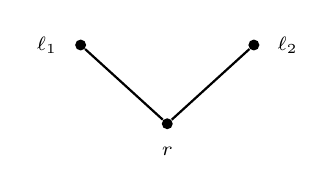
\begin{tikzpicture}[
  vertex/.style={circle, fill=black, inner sep=1.4pt},
  vedge/.style={thick},
  vlabel/.style={font=\scriptsize}
]
\node[vertex] (root) at (0,0) {};
\node[vlabel, below=1mm of root] {$r$};
\node[vertex] (lefta) at (-1.1,1.0) {};
\node[vlabel, left=1mm of lefta] {$\ell_1$};
\node[vertex] (righta) at (1.1,1.0) {};
\node[vlabel, right=1mm of righta] {$\ell_2$};
\draw[vedge] (root) -- (lefta);
\draw[vedge] (root) -- (righta);
\end{tikzpicture}
\end{center}

\[
\begin{array}{rcl}
\rho(r) &=& \wedge R, \qquad \sigma(r) = \Gamma \ms ((A\Rightarrow B)\wedge C),\Theta,\\[1mm]
\rho(\ell_1) &=& \textsc{Base}, \qquad \sigma(\ell_1) = \Gamma \ms (A\Rightarrow B),\Theta,\\[1mm]
\rho(\ell_2) &=& \textsc{Base}, \qquad \sigma(\ell_2) = \Gamma \ms C,\Theta.
\end{array}
\]

\noindent Formally, this is the same proof object viewed as a finite rooted
ordered tree \((V,E,r)\) together with a sequent-labelling map
\(\sigma : V \to \Seq(L)\) and a rule-labelling map
\[
\rho:V\to\{\mathsf{Base},\Rightarrow L,\Rightarrow R,\wedge L,\wedge R,\vee L,\vee R,\neg L,\neg R\}.
\]
If \(v\) is an internal vertex with ordered children \(v_1,\dots,v_n\), then
\(\sigma(v_1),\dots,\sigma(v_n)\) are exactly the premisses of an instance of
the rule \(\rho(v)\) with conclusion \(\sigma(v)\). If \(v\) is a leaf, then
\(\rho(v)=\mathsf{Base}\), and \(\sigma(v)\) is justified by a primitive
consequence instance.

\medskip



\subsection{Induced derivability}

\begin{definition}
For \(\Gamma,\Delta\in \MSet(L)\), we write
\[
\Gamma \vdash_{\NMMS(\mszero)} \Delta
\]
if there exists a derivation of the sequent \(\Gamma \ms \Delta\) in the
calculus \(\NMMS(\mszero)\).
\end{definition}

\begin{remark}
The distinction between the primitive $\mszero$ and the induced derivability $\vdash_{\NMMS(\mszero)}$ is mathematically significant in the nonmonotonic setting: the latter is not in general a monotone extension of the former. The passage $\mszero \leadsto \vdash_{\NMMS(\mszero)}$ is the proof-theoretic closure from primitive material consequence to full derivability.
\end{remark}

\section{Proof trees}

\subsection{Tree representation}

\begin{definition}
A \emph{proof tree} is a tuple
\[
t=(V_t,E_t,r_t,\lambda_t,\sigma_t),
\]
where \((V_t,E_t,r_t)\) is a finite rooted ordered tree,
\(\sigma_t:V_t\to \Seq(L)\) is a sequent-labelling, and
\[
\lambda_t:V_t\to
\{\mathsf{Base},\Rightarrow L,\Rightarrow R,\wedge L,\wedge R,\vee L,\vee R,\neg L,\neg R\},
\]
such that:
\begin{enumerate}[label=\textup{(\roman*)}]
\item if \(v\) is a leaf, then \(\lambda_t(v)=\mathsf{Base}\);
\item if \(v\) is an internal vertex, then \(\lambda_t(v)\neq \mathsf{Base}\),
and the ordered immediate subtrees of \(v\) are exactly the premise trees of
an instance of the rule \(\lambda_t(v)\) with conclusion equal to the sequent
label of \(v\).
\end{enumerate}
The sequent at the root is called the \emph{conclusion} of the proof tree.
\end{definition}

\begin{remark}
The order on immediate subtrees is part of the formal object, which is why
addresses are later indexed by finite sequences of child indices.
Conceptually, these are ordinary rooted proof trees.
\end{remark}

\begin{proposition}
Every derivation \(d\) in \(\NMMS(\mszero)\) determines a proof tree
\(\Tree(d)\) with the same conclusion sequent.
\end{proposition}

\begin{proof}
We argue by induction on the height of the derivation \(d\).

If \(d\) has height \(0\), then \(d\) is a base derivation
\[
\frac{\Gamma \mszero \Theta}{\Gamma \ms \Theta}.
\]
We assign to \(d\) the one-vertex rooted tree whose unique vertex is labelled
by the sequent \(\Gamma \ms \Theta\) and tagged by \(\mathsf{Base}\). Its root
label is therefore the conclusion sequent of \(d\).

Suppose now that \(d\) ends with an application of one of the logical rules of
\(\NMMS(\mszero)\), with immediate subderivations \(d_1,\dots,d_n\). By the
induction hypothesis, each \(d_i\) determines a finite rooted ordered proof
tree \(\Tree(d_i)\) whose root carries the conclusion sequent of \(d_i\). Form
a new rooted ordered tree by adjoining a fresh root \(r\), declaring the trees
\(\Tree(d_1),\dots,\Tree(d_n)\) to be the ordered immediate subtrees of \(r\),
labelling \(r\) by the conclusion sequent of the last inference of \(d\), and
tagging \(r\) by the rule symbol used in that inference.

Because the premiss sequents of the last rule instance are exactly the
conclusion sequents of the subderivations \(d_1,\dots,d_n\), the resulting
rooted ordered tree satisfies the defining conditions of a proof tree. It is
finite because it is obtained by adjoining one new root to finitely many finite
trees. Its root sequent is, by construction, the conclusion sequent of \(d\).

This completes the induction.
\end{proof}

\begin{definition}[The set of proof trees]
We write \(\PTree\) for the set of all finite rooted ordered trees equipped
with the rule labels and sequent labels induced by derivations of
\(\NMMS(\mszero)\). Thus an element \(t\in\PTree\) may be written as
\[
t=(V_t,E_t,r_t,\lambda_t,\sigma_t),
\]
where \(V_t\) is the finite vertex set, \(E_t\subseteq V_t\times V_t\) is the
edge relation directed away from the root \(r_t\), \(\lambda_t\) records the
rule label at each vertex, and \(\sigma_t\) records the sequent label. When
the labels play no explicit role we suppress them and write simply
\(t=(V_t,E_t,r_t)\).
\end{definition}

\begin{remark}
All trees occurring below are elements of \(\PTree\). In particular, the raw
grafting product and its linearization are defined on \(\PTree\) itself; the
quotient enters later at the level of \emph{two-step witnesses} for the
associator, not at the level of the underlying one-step product.
\end{remark}

\paragraph{Small shapes.}
As in the usual Hopf algebras of rooted trees, it is helpful to keep the first
few shapes in view.  The following pictures suppress sequent labels and rule
tags; they show only the underlying rooted ordered tree.  In our setting the
allowed labels on the root determine the arity: base axioms give leaves,
unary logical rules give one-child nodes, and binary logical rules give
two-child nodes.

\begin{center}
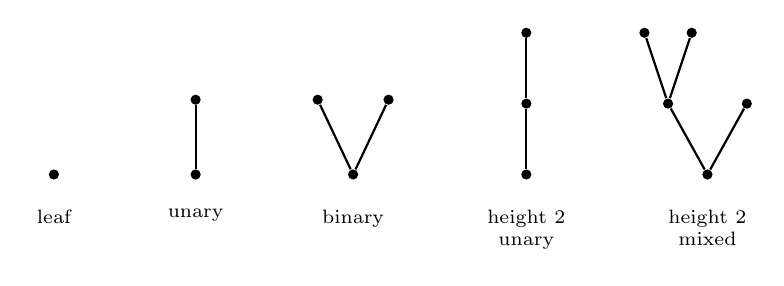
\begin{tikzpicture}[
  nd/.style={circle,fill=black,inner sep=1.3pt},
  ed/.style={thick},
  lab/.style={font=\scriptsize,align=center}
]
\begin{scope}[shift={(-4.5,0)}]
  \node[nd] (r) at (0,0) {};
  \node[lab,below=2.5mm of r] {leaf};
\end{scope}
\begin{scope}[shift={(-2.7,0)}]
  \node[nd] (r) at (0,0) {};
  \node[nd] (a) at (0,0.95) {};
  \draw[ed] (r)--(a);
  \node[lab,below=2.5mm of r] {unary};
\end{scope}
\begin{scope}[shift={(-0.7,0)}]
  \node[nd] (r) at (0,0) {};
  \node[nd] (a) at (-0.45,0.95) {};
  \node[nd] (b) at (0.45,0.95) {};
  \draw[ed] (r)--(a); \draw[ed] (r)--(b);
  \node[lab,below=2.5mm of r] {binary};
\end{scope}
\begin{scope}[shift={(1.5,0)}]
  \node[nd] (r) at (0,0) {};
  \node[nd] (a) at (0,0.9) {};
  \node[nd] (b) at (0,1.8) {};
  \draw[ed] (r)--(a); \draw[ed] (a)--(b);
  \node[lab,below=2.5mm of r] {height $2$\\unary};
\end{scope}
\begin{scope}[shift={(3.8,0)}]
  \node[nd] (r) at (0,0) {};
  \node[nd] (a) at (-0.5,0.9) {};
  \node[nd] (b) at (0.5,0.9) {};
  \node[nd] (c) at (-0.8,1.8) {};
  \node[nd] (d) at (-0.2,1.8) {};
  \draw[ed] (r)--(a); \draw[ed] (r)--(b);
  \draw[ed] (a)--(c); \draw[ed] (a)--(d);
  \node[lab,below=2.5mm of r] {height $2$\\mixed};
\end{scope}
\end{tikzpicture}
\end{center}

\noindent
For a fixed number of vertices there are only finitely many underlying ordered
shapes, but each shape supports many proof trees because its vertices may be
decorated by different sequents and rule tags.  The algebra below is therefore
not the ordinary Grossman--Larson algebra on bare trees; it is the same kind
of rooted-tree combinatorics carried by proof-theoretic decorations and exact
sequent interfaces.

\subsection{Rule arity, height, and proof-tree induction}

The rules of $\NMMS(\mszero)$ divide by number of premisses: Base has arity~$0$; the unary rules $\Rightarrow R$, $\wedge L$, $\vee R$, $\neg L$, $\neg R$ have arity~$1$; and the binary rules $\Rightarrow L$, $\wedge R$, $\vee L$ have arity~$2$. A proof tree is \emph{arity-correct} if every vertex has exactly as many children as its rule arity demands.

\begin{theorem}[Derivation trees respect rule arity]
If \(d\) is a derivation of \(\NMMS(\mszero)\), then the associated proof tree
\(\Tree(d)\) is arity-correct.
\end{theorem}

\begin{proof}
The proof is by induction on the final rule of \(d\). A base derivation is sent
to a one-vertex tree, and \(\alpha(\mathsf{Base})=0\). If \(d\) ends with a
logical rule \(R\) with premisses \(d_1,\ldots,d_n\), then the construction of
\(\Tree(d)\) adjoins a new root whose children are exactly
\(\Tree(d_1),\ldots,\Tree(d_n)\). By the definition of the inference rules,
\(n=\alpha(R)\), and by the induction hypothesis the children are themselves
arity-correct.
\end{proof}

\begin{definition}[Tree height]
The \emph{height} \(h(t)\) of a proof tree is defined recursively by
\[
h(t)=0
\quad\text{if }t\text{ is a leaf},
\]
and, if \(t\) has immediate subtrees \(t_1,\ldots,t_n\),
\[
h(t)=1+\max\{h(t_i):1\le i\le n\}.
\]
The empty maximum does not occur in the second clause, since leaves are treated
by the first clause.
\end{definition}

\begin{theorem}[Derivation height equals tree height]
For every derivation \(d\),
\[
h(\Tree(d))=\operatorname{height}(d).
\]
\end{theorem}

\begin{proof}
Again argue by induction on \(d\). The base case is immediate. In the inductive
case, the height of the derivation is one plus the maximum height of its
immediate subderivations, and the height of the associated tree is one plus the
maximum height of the corresponding immediate subtrees. The induction
hypothesis identifies these two maxima.
\end{proof}

\begin{corollary}[Induction principles]
Any property \(P(t)\) of proof trees which is preserved by adjoining a
rule-labelled root above arity-correct child trees may be proved for all
derivation trees by induction on derivation height, equivalently by induction
on tree height. Concretely, it suffices to prove:
\begin{enumerate}[label=\textup{(\roman*)}]
\item \(P(t)\) for every base leaf;
\item for each rule \(R\) of arity \(n\), if \(P(t_i)\) holds for
arity-correct proof trees \(t_1,\ldots,t_n\), then \(P(R(t_1,\ldots,t_n))\)
holds.
\end{enumerate}
\end{corollary}

\begin{remark}
The induction is not over arbitrary \(n\)-ary trees but over rule-labelled
trees whose branching is controlled by the logical rule at the root.
The cases decompose by inference rule, with the number of children fixed
by rule arity. This is the proof-theoretically natural induction measure,
and it is what makes the algebraic combinatorics tractable.
\end{remark}

\subsection{Addresses}

\begin{definition}
An \emph{address} in a proof tree is a finite sequence of natural numbers
indicating a path from the root by successive child indices. The empty address
selects the whole tree.
\end{definition}

\begin{definition}[Address set and vertex map]
If \(t=(V_t,E_t,r_t)\) is a rooted ordered proof tree, we write
\[
\Addr(t)\subseteq \mathbb N^{<\omega}
\]
for the set of all finite sequences \(a=(a_1,\dots,a_n)\) for which there
exists a chain of vertices
\[
v_0=r_t,\ v_1,\dots,v_n\in V_t
\]
such that, for each \(i<n\), the vertex \(v_{i+1}\) is the \(a_{i+1}\)-th
element of the ordered child list \(\operatorname{ch}_t(v_i)\). The empty
sequence \(\langle\rangle\) belongs to \(\Addr(t)\) and names the root. We write
\[
v_t:\Addr(t)\to V_t
\]
for the induced vertex map, sending an address to the corresponding vertex.
If \(a,c\in \mathbb N^{<\omega}\), we write \(a\cdot c\) for concatenation of
addresses. For addresses \(a,b\), we write \(a\preceq b\) if \(a\) is an
initial segment of \(b\), and \(a\prec b\) if \(a\preceq b\) and \(a\neq b\).
Thus \(b\) \emph{extends} \(a\) exactly when \(a\preceq b\). Two addresses are
\emph{incomparable} if neither \(a\preceq b\) nor \(b\preceq a\).
\end{definition}

\begin{remark}
Addresses are not conceptually basic; they are a bookkeeping device for
locating graft sites and comparing nested versus parallel graft regimes.
\end{remark}

\begin{definition}[Address cones and rooted subtrees]
Let \(t\in \PTree\) and \(a\in \Addr(t)\). The \emph{address cone below \(a\)}
is the principal upset
\[
\Addr_t(a):=\{\,b\in \Addr(t)\mid a\preceq b\,\}.
\]
The \emph{rooted subtree of \(t\) at \(a\)} is denoted \(t\downarrow_a\). Its
address set is
\[
\Addr(t\downarrow_a)
:=
\{\,c\in \mathbb N^{<\omega}\mid a\cdot c\in \Addr(t)\,\},
\]
and its rule and sequent labels are inherited from those of \(t\) along the
translation \(c\mapsto a\cdot c\).
\end{definition}

\begin{proposition}[Disjointness of incomparable address cones]\label{prop:disjoint-cones}
Let \(t\in\PTree\) and \(a,b\in \Addr(t)\). If \(a\) and \(b\) are
incomparable, then
\[
\Addr_t(a)\cap \Addr_t(b)=\varnothing.
\]
\end{proposition}

\begin{proof}
Suppose \(d\in \Addr_t(a)\cap \Addr_t(b)\). Then \(a\preceq d\) and
\(b\preceq d\). Since \(a\) and \(b\) are both initial segments of the same
finite sequence \(d\), one of them must be an initial segment of the other.
Hence \(a\preceq b\) or \(b\preceq a\), contradicting incomparability.
\end{proof}

\begin{remark}[Finiteness of address chains]
For each fixed proof tree \(t\), the set \(\Addr(t)\) is finite, since the
vertex set \(V_t\) is finite and the vertex map \(v_t:\Addr(t)\to V_t\) is
bijection onto the vertices of \(t\). Hence \((\Addr(t),\preceq)\) is a finite
partially ordered set. In particular, every chain
\[
a_0 \prec a_1 \prec \cdots \prec a_k
\]
of comparable addresses is finite. Thus for any fixed derivation, iterated
nesting of graft sites may occur only finitely many times: one can move
strictly downward in the tree only along a finite address chain.
\end{remark}

\begin{remark}[Use of cones in the two-step analysis]
The notations \(\Addr_t(a)\) and \(t\downarrow_a\) are used later in the
graft-pair decomposition. If
\[
\graftat{z}{a}{y}=z'
\qquad\text{and}\qquad
\graftat{z'}{b}{x}=w,
\]
then the \emph{inner} case is the condition \(b\in \Addr_{z'}(a)\), i.e.
\(a\preceq b\), while the \emph{outer} case is the condition that \(a\) and
\(b\) are incomparable in \((\Addr(z'),\preceq)\). Proposition~\ref{prop:disjoint-cones} is exactly
the set-theoretic statement that the rooted regions affected by two outer
grafts are disjoint.
\end{remark}

% ---- Proof tree with address labels ----
\begin{center}
\begin{tikzpicture}[
  nd/.style={circle,fill=black,inner sep=1.4pt},
  ed/.style={thick},
  seq/.style={font=\scriptsize,inner sep=1pt},
  adr/.style={font=\scriptsize\ttfamily,color=gray!70!black}
]
\node[nd] (r)  at ( 0,  0) {};
\node[nd] (l)  at (-2.2,1.5) {};
\node[nd] (rr) at ( 2.2,1.5) {};
\node[nd] (ll) at (-2.2,3.0) {};
\draw[ed] (r)--(l); \draw[ed] (r)--(rr); \draw[ed] (l)--(ll);
\node[seq,below=2mm of r]  {$\wedge R,\;\Gamma\ms(A\wedge B),\Theta$};
\node[adr,left=1mm of r]   {\texttt{[]}};
\node[seq,left=1.5mm of l] {$\vee R,\;\Gamma\ms(A\vee B),\Theta$};
\node[adr,above=1mm of l]  {\texttt{[0]}};
\node[seq,right=1.5mm of rr]{\textsc{Base},\;$\Gamma\ms B,\Theta$};
\node[adr,above=1mm of rr] {\texttt{[1]}};
\node[seq,left=1mm of ll]  {\textsc{Base},\;$\Gamma\mszero A,B,\Theta$};
\node[adr,above=1mm of ll] {\texttt{[0,0]}};
\end{tikzpicture}
\end{center}
\noindent\small
Addresses (grey \texttt{monospace}) record paths from the root by child index.
Leaves at \texttt{[0,0]} and \texttt{[1]} are open premiss positions.

\section{Matching-leaf grafting}

The next step is to turn proof substitution into an algebraic operation.  The
operation is more rigid than ordinary rooted-tree insertion: a
tree may be inserted only at a leaf whose sequent label is exactly the
conclusion sequent of the tree being inserted.  In a system admitting
weakening, one could freely enlarge any leaf's context to match an
arbitrary insertion target, making all graft sites universally accessible.
Here weakening is absent, so context interfaces cannot be stretched:
each graft site must be earned by exact sequent agreement.  This is the
point at which the failure of monotonicity of \(\mszero\) becomes
directly visible in the algebra, and it is what makes the resulting
product structurally non-trivial.

\paragraph{Matching leaves.}
Let \(x,t\in\PTree\).  We write
\[
\operatorname{Leaf}_x(t)
\]
for the finite set of leaves \(a\in\Addr(t)\) whose sequent label is the
root sequent of \(x\).  For \(a\in\operatorname{Leaf}_x(t)\), let
\[
\operatorname{gr}_a(x,t)
\]
be the proof tree obtained by replacing the leaf \(a\) of \(t\) by the whole
tree \(x\).  Since the conclusion of \(x\) is exactly the sequent carried by
the leaf, this replacement preserves correctness of the surrounding rule
instance.  Thus \(\operatorname{gr}_a(x,t)\) is again a proof tree.

\begin{proposition}[Closure under matching-leaf grafting]
If \(x\) and \(t\) are proof trees of \(\NMMS(\mszero)\) and
\(a\in\operatorname{Leaf}_x(t)\), then \(\operatorname{gr}_a(x,t)\) is again
the proof tree of a derivation of \(\NMMS(\mszero)\).
\end{proposition}

\begin{proof}
The leaf at \(a\) is a base-premiss occurrence whose sequent label agrees with
the conclusion of \(x\).  Replacing that leaf by the derivation tree \(x\)
therefore preserves the premiss expected by the parent inference rule.  All
other vertices and rule instances are unchanged.  Reading the resulting tree
from leaves to root gives a derivation with the same conclusion as \(t\).
\end{proof}

\paragraph{Linearization.}
Let \(V=\ZZ\langle\PTree\rangle\) be the free abelian group on proof trees.
For basis trees define
\[
x\triangleright t
:=
\sum_{a\in\operatorname{Leaf}_x(t)}
\operatorname{gr}_a(x,t),
\]
and extend bilinearly to \(V\).  The sum is finite because \(t\) has finitely
many leaves.  This is the proof-theoretic analogue of the Grossman--Larson
insertion product: one inserts \(x\) into all admissible sites of \(t\), but
the admissible sites are determined by exact sequent-interface matching.

\paragraph{Running example.}
Suppose \(t\) has two open leaves carrying the same sequent \(\Gamma\ms\Delta\),
and \(x\) is a derivation of \(\Gamma\ms\Delta\).  Then
\[
x\triangleright t
=
\operatorname{gr}_{a_1}(x,t)+\operatorname{gr}_{a_2}(x,t),
\]
one term for each matching open leaf.  If a third leaf differs only by an
extra formula in the context, it is not a matching site: without weakening one
cannot enlarge or shrink interfaces in order to force a graft.

\medskip

\noindent Here is the same operation with the proof-theoretic labels visible.
The left tree \(t\) has an open base leaf labelled
\(\Gamma \ms (A\vee B),\Theta\).  The middle tree \(u\), drawn in red, derives
that exact sequent.  Grafting replaces the matching leaf of \(t\) by the
whole derivation \(u\).

\begin{center}
\begin{minipage}{0.42\textwidth}
\centering
\[
\begin{prooftree}
\hypo{\Gamma \mszero (A\vee B),\Theta}
\infer1[\textsc{Base}]{\Gamma \ms (A\vee B),\Theta}
\hypo{\Gamma \mszero C,\Theta}
\infer1[\textsc{Base}]{\Gamma \ms C,\Theta}
\infer2[\(\wedge R\)]{\Gamma \ms ((A\vee B)\wedge C),\Theta}
\end{prooftree}
\]
\small \(t\)
\end{minipage}
\hfill
\begin{minipage}{0.32\textwidth}
\centering
\[
\begin{prooftree}
\hypo{\Gamma \mszero A,B,\Theta}
\infer1[\textsc{Base}]{\Gamma \ms A,B,\Theta}
\infer1[\(\vee R\)]{\Gamma \ms (A\vee B),\Theta}
\rewrite{\color{red}\box\treebox}
\end{prooftree}
\]
\small \(u\)
\end{minipage}
\end{center}

\begin{center}
\[
\begin{prooftree}
\hypo{\Gamma \mszero A,B,\Theta}
\infer1[\textsc{Base}]{\Gamma \ms A,B,\Theta}
\infer1[\(\vee R\)]{\Gamma \ms (A\vee B),\Theta}
\rewrite{\color{red}\box\treebox}
\hypo{\Gamma \mszero C,\Theta}
\infer1[\textsc{Base}]{\Gamma \ms C,\Theta}
\infer2[\(\wedge R\)]{\Gamma \ms ((A\vee B)\wedge C),\Theta}
\end{prooftree}
\]
\small \(\operatorname{gr}_a(u,t)\)
\end{center}

\medskip

\noindent The graph-theoretic picture is the same substitution with labels
suppressed.  The blue vertex marks the matching leaf in \(t\), the red tree is
the inserted derivation \(u\), and the right-hand tree shows the inserted
branch in red.

\begin{center}
\begin{tikzpicture}[
  vertex/.style={circle, fill=black, inner sep=1.4pt},
  redvertex/.style={circle, fill=red, inner sep=1.4pt},
  bluevertex/.style={circle, fill=blue!70!black, inner sep=1.6pt},
  vedge/.style={thick},
  rededge/.style={thick, red},
  lab/.style={font=\scriptsize, inner sep=1pt}
]
\node at (-3.5,2.5) {$t$};
\node[vertex] (tr) at (-3.5,0) {};
\node[vertex] (ta) at (-4.2,1.1) {};
\node[bluevertex] (tl) at (-2.8,1.1) {};
\draw[vedge] (tr) -- (ta);
\draw[vedge] (tr) -- (tl);
\node[lab, right=0.7mm of tl, text=blue!70!black] {$s$};

\node at (0,2.5) {$u$};
\node[redvertex] (ur) at (0,0) {};
\node[redvertex] (ua) at (-0.6,1.1) {};
\draw[rededge] (ur) -- (ua);
\node[lab, below=1mm of ur, text=red] {$s$};

\node at (3.5,2.5) {$\operatorname{gr}_a(u,t)$};
\node[vertex] (gr) at (3.5,0) {};
\node[vertex] (ga) at (2.8,1.1) {};
\node[redvertex] (gu) at (4.2,1.1) {};
\node[redvertex] (gua) at (4.8,2.2) {};
\draw[vedge] (gr) -- (ga);
\draw[vedge] (gr) -- (gu);
\draw[rededge] (gu) -- (gua);
\node[lab, right=0.7mm of gu, text=blue!70!black] {$s$};

\node at (-1.75,1.1) {$\leadsto$};
\node at (1.75,1.1) {$\leadsto$};
\end{tikzpicture}
\end{center}

\section{Associators and the geometry of two grafts}

The pre-Lie identity is a statement about associators.  In the present setting
the relevant combinatorics is not the full syntax of derivations, but the
relative position of two graft sites in a rooted tree.

\paragraph{Two-step grafts.}
Consider a two-step composite
\[
\operatorname{gr}_b(x,\operatorname{gr}_a(y,z)).
\]
The first graft inserts \(y\) into \(z\) at \(a\).  The second graft inserts
\(x\) into the resulting tree at \(b\).  There are only two possible geometric
regimes.

\begin{theorem}[Two-step decomposition]
Let \(z'=\operatorname{gr}_a(y,z)\), and suppose \(b\) is a matching leaf of
\(z'\) for \(x\).  Then exactly one of the following holds.
\begin{enumerate}[label=\textup{(\roman*)}]
\item \emph{Nested case.}  The address \(b\) lies inside the copy of \(y\)
inserted at \(a\).  Equivalently, \(b=a\cdot c\) for a unique nonempty address
\(c\in\Addr(y)\).  In this case
\[
\operatorname{gr}_{a\cdot c}(x,\operatorname{gr}_a(y,z))
=
\operatorname{gr}_a(\operatorname{gr}_c(x,y),z).
\]
\item \emph{Parallel case.}  The addresses \(a\) and \(b\) are incomparable.
In this case the two local substitutions commute:
\[
\operatorname{gr}_b(x,\operatorname{gr}_a(y,z))
=
\operatorname{gr}_a(y,\operatorname{gr}_b(x,z)).
\]
\end{enumerate}
\end{theorem}

\begin{proof}
The address \(a\) becomes the root address of the inserted copy of \(y\) in
\(z'\).  If \(b\) extends \(a\), then \(b=a\cdot c\) for a unique address
\(c\) of \(y\).  The case \(c=\langle\rangle\) would graft \(x\) at the root of
the inserted copy rather than at a leaf inside it, so for a genuine second
graft inside \(y\) the extension is nonempty.  Locality of replacement gives
the displayed nested identity.

If \(b\) does not extend \(a\), then \(b\) cannot be a strict prefix of \(a\):
the address \(b\) is a leaf of \(z'\), and no valid address can lie strictly
below a leaf.  Hence \(a\) and \(b\) are incomparable.  The rooted subtrees at
incomparable addresses are disjoint, so replacing one leaves the other
unchanged.  Therefore the two replacements commute.
\end{proof}

\paragraph{Bureaucracy.}
The same final two-step proof tree may be presented by different ordered
histories.  In the parallel case, the two histories differ only by the order
in which two independent substitutions are performed.  In the nested case,
one may either first form an inner composite and then insert it, or insert the
outer tree first and then work inside it.  We write \(\sim_{\mathrm b}\) for
the equivalence relation on two-step graft histories generated by these two
local identifications.  Each generator preserves the terminal proof tree.

\begin{remark}
This is the proof-theoretic analogue of quotienting away bureaucratic
permutations of independent inferences.  It is close in spirit to the passage
from sequent derivations to proof nets, but here the quotient is used only to
organize the associator comparison.
\end{remark}

\section{The pre-Lie theorem}

For \(x,y,z\in\PTree\), write
\[
A(x,y,z):=(x\triangleright y)\triangleright z
-x\triangleright (y\triangleright z)
\]
for the right associator of the grafting product.

\begin{theorem}[Grafting is right pre-Lie]\label{thm:prelie}
The bilinear product \(\triangleright\) on \(V=\ZZ\langle\PTree\rangle\)
satisfies
\[
A(x,y,z)=A(x,z,y)
\]
for all proof trees \(x,y,z\).  Hence \(V\) is a right pre-Lie algebra.
\end{theorem}

\begin{proof}
By bilinearity it suffices to compare coefficients of a fixed output tree
\(w\).  Such a coefficient is counted by two-step graft histories with terminal
tree \(w\).

The two-step decomposition separates these histories into nested and parallel
regimes.  Nested histories are exactly those accounted for by the subtraction
term \(x\triangleright(y\triangleright z)\): they amount to first inserting
\(x\) into \(y\), then inserting the result into \(z\).  Thus the nested
contribution is removed from the associator, leaving only the parallel regime.

The remaining histories are parallel: the two insertions occur at mutually
incomparable addresses of the same receiver tree.  We pass to a quotient of
two-step graft histories, identifying those that differ only by the
serialisation of such independent concurrent operations.  In each equivalence
class under this quotient, one may exchange the roles of \(y\) and \(z\)
without changing the terminal tree: the class governed by inserting \(y\)
at \(a\) and \(x\) at a site in the unchanged portion of \(z\) corresponds
exactly, under commutation at incomparable addresses, to the class in
\(A(x,z,y)\) governed by the same pair of sites with \(y\) and \(z\)
exchanged.

Concretely: the quotient separates contributions into a \emph{noise sector}
--- histories that are trivial modulo the parallel-commutativity equivalence
and cancel across the two bracketings --- and a \emph{residual sector} of
genuinely asymmetric contributions.  The noise sector contributes equally to
\(A(x,y,z)\) and \(A(x,z,y)\) and so drops out.  In the residual sector the
exchange of \(y\) and \(z\) gives an explicit sign-preserving bijection
between contribution classes.  Therefore the coefficients of every output
tree \(w\) agree across the two bracketings, and \(A(x,y,z)=A(x,z,y)\).
\end{proof}

\begin{remark}
The formal development proves this comparison at the level of quotient classes
of two-step histories.  The quotient is not an extra algebraic carrier; it is
the identity criterion used in the associator proof.  The one-step product is
the raw grafting product on proof trees.
\end{remark}

\begin{corollary}[The induced Lie algebra]\label{cor:lie}
The commutator
\[
[x,y]:=x\triangleright y-y\triangleright x
\]
defines a Lie bracket on \(V\).
\end{corollary}

\begin{proof}
Every right pre-Lie algebra has a Lie algebra commutator.  Antisymmetry is
immediate, and the Jacobi identity is the standard cancellation obtained by
expanding the pre-Lie identity in the three cyclic orders.
\end{proof}

\begin{remark}
The Lie bracket \([x,y]=x\triangleright y-y\triangleright x\) has a
direct proof-theoretic reading: it measures the \emph{asymmetry of proof
substitution}.  The term \(x\triangleright y\) inserts \(x\) into the open
premiss positions of \(y\); the term \(y\triangleright x\) does the reverse.
Their difference records which insertions are available in one direction
but not the other --- a quantity that is non-trivial precisely because
the leaf-matching constraint is sensitive to the direction of substitution.
That this difference satisfies the Jacobi identity is a structural theorem
about the proof-tree algebra, not merely an algebraic formality.
\end{remark}

\section{Relation with rooted-tree Hopf algebras}

The construction above is the proof-theoretic analogue of a familiar
rooted-tree story.  For ordinary rooted trees, insertion at vertices defines a
pre-Lie algebra; its commutator is the Grossman--Larson Lie algebra; and the
universal enveloping algebra is a Hopf algebra.  The proof-theoretic novelty is
that the insertion sites are not arbitrary vertices: they are matching
premiss-leaves determined by the primitive consequence relation.

\paragraph{Forests and the symmetric algebra.}
Let \(\Forest(\PTree)\) be the free commutative monoid on proof trees, with
unit the empty forest \(1\).  The free commutative algebra
\[
\ZZ[\Forest(\PTree)]\cong S_{\ZZ}(V)
\]
is the symmetric algebra on \(V\).  A forest is not itself a single proof; it
is the algebraic carrier on which the Hopf algebra lives.

\begin{theorem}[Oudom--Guin]
Let \(A\) be a right pre-Lie algebra.  The symmetric algebra \(S(A)\) carries
an associative product \(\star\), determined by the pre-Lie action, for which
\[
\Delta(a)=a\otimes 1+1\otimes a\qquad(a\in A)
\]
extends to a coproduct making \(S(A)\) a Hopf algebra.  This Hopf algebra is
canonically isomorphic to the universal enveloping algebra of the Lie algebra
associated to \(A\).
\end{theorem}

\paragraph{The algebraic structure explicitly.}
Applied to \(A=V\), the Oudom--Guin construction gives the following concrete
objects.  The underlying module is the symmetric algebra
\[
S(V)=\ZZ[\Forest(\PTree)].
\]
Its unit is the empty forest \(1\).  The product \(\star\) is the unique
Oudom--Guin product extending the proof-tree pre-Lie operation: on generators
it records insertion/grafting, and on forests it is extended by the recursive
Oudom--Guin rule.  The coproduct is the primitive-generator coproduct,
extended as an algebra morphism from the commutative forest algebra:
\[
\Delta(1)=1\otimes 1,
\qquad
\Delta(x)=x\otimes 1+1\otimes x
\quad(x\in V),
\]
and therefore, for a forest \(x_1\cdots x_n\),
\[
\Delta(x_1\cdots x_n)
=
\sum_{I\sqcup J=\{1,\ldots,n\}}
\Bigl(\prod_{i\in I}x_i\Bigr)\otimes
\Bigl(\prod_{j\in J}x_j\Bigr).
\]
The counit is
\[
\varepsilon(1)=1,\qquad
\varepsilon(F)=0
\quad\text{for every nonempty forest }F.
\]

\begin{proposition}[The Oudom--Guin bialgebra]
With the product \(\star\), unit \(1\), coproduct \(\Delta\), and counit
\(\varepsilon\) above, \(S(V)\) is a connected graded bialgebra.
\end{proposition}

\begin{proof}
Associativity of \(\star\) and compatibility of \(\star\) with the primitive
coproduct are precisely the Oudom--Guin theorem; the pre-Lie identity is the
hypothesis needed for that construction.  Coassociativity of \(\Delta\) on
generators follows from
\[
(\Delta\otimes \mathrm{id})\Delta(x)
=x\otimes 1\otimes 1+1\otimes x\otimes 1+1\otimes 1\otimes x
=(\mathrm{id}\otimes\Delta)\Delta(x),
\]
and hence on all forests because \(\Delta\) is multiplicative.  The counit
identities are immediate on \(1\) and on primitive generators, and again
extend multiplicatively.  The grading is by forest length or, equivalently,
by total proof-tree weight; the degree-zero part is \(\ZZ\cdot 1\), so the
bialgebra is connected.
\end{proof}

\begin{theorem}[Antipode]
The connected graded bialgebra \(S(V)\) has a unique antipode \(S\).  It is
defined recursively by
\[
S(1)=1,
\qquad
S(F)=-F-\sum S(F')\star F'',
\]
where the sum ranges over the reduced coproduct
\[
\widetilde{\Delta}(F)
=\Delta(F)-F\otimes 1-1\otimes F
=\sum F'\otimes F''.
\]
It satisfies
\[
m_\star(S\otimes \mathrm{id})\Delta
=
\eta\varepsilon
=
m_\star(\mathrm{id}\otimes S)\Delta.
\]
\end{theorem}

\begin{proof}
This is the standard antipode construction for connected graded bialgebras.
The reduced coproduct of a homogeneous element of positive degree has tensor
factors of strictly smaller degree, so the displayed recursion is well-founded
on degree.  An induction on degree then shows that convolution with the
identity gives the unit-counit map on both sides.  Uniqueness follows from the
same induction: any convolution inverse of the identity must satisfy the
recursive formula.
\end{proof}

\begin{corollary}[The Oudom--Guin Hopf algebra of proof trees]\label{cor:hopf}
The pre-Lie algebra \((V,\triangleright)\) of proof trees determines a Hopf
algebra on \(S(V)\).  Its primitive generators are the proof trees, and its
Lie algebra of primitives is generated by the proof-theoretic commutator
\([x,y]=x\triangleright y-y\triangleright x\).
\end{corollary}

\begin{remark}[Proof-theoretic content of the Hopf structure]
Each component of the Hopf algebra has a direct proof-theoretic reading.
The \emph{product} \(\star\) on \(S(V)\) is proof composition extended to
forests: combining collections of derivations.  The \emph{coproduct}
\(\Delta(t)=t\otimes 1+1\otimes t\) expresses the fact that, in the absence
of weakening and contraction, each proof tree is an \emph{atomic} or
\emph{primitive} proof-theoretic object: it cannot be split into genuinely
independent sub-components by any structural decomposition.  This
primitivity is a consequence of the non-monotone constraint --- it is the
absence of structural rules that prevents non-trivial decomposition.  The
\emph{antipode} provides a formal inverse for proof composition, whose
existence follows from the connected graded structure (graded by derivation
height).  The \emph{Lie bracket} \([x,y]\) records the directional
asymmetry of proof substitution described above.

This construction should be distinguished from the Connes--Kreimer cut
coproduct, in which the coproduct is defined by admissible cuts of trees
and encodes genuine proof decomposition.  The two coproducts are related
but distinct.  The Oudom--Guin Hopf algebra established here is the
algebraic structure that the pre-Lie proof-tree product determines; the
cut coproduct and its relation to the primitive-generator coproduct is a
separate problem, discussed briefly in the following section.
\end{remark}

\begin{remark}[Two Hopf algebras]
The Oudom--Guin construction yields $H_{\mathrm{OG}}$ with the grafting product $\star$ and the primitive coproduct $\Delta(t)=t\otimes 1+1\otimes t$.  There is a second Hopf algebra $H_{\mathrm{split}}$ with the forest-union product and the admissible-cut coproduct $\Delta_{\mathrm{split}}$.  These are \emph{not} the same algebra: $H_{\mathrm{OG}}$ encodes the \emph{building} of proofs by grafting; $H_{\mathrm{split}}$ encodes the \emph{decomposition} of proofs by cutting.  Sections~8--10 develop $H_{\mathrm{split}}$ and the duality between the two.
\end{remark}

\section{Hypersequents and the splitting structure}

\subsection{Hypersequents for NMMS}

A \emph{hypersequent} (Avron~\cite{avron1996hypersequents}) is a finite multiset of sequents, written
\[
S_1 \mid S_2 \mid \cdots \mid S_n.
\]
Each $S_i$ is an individual sequent of $\NMMS(\mszero)$; the pipe $\mid$ is an external separator with no internal logical content.  In the standard hypersequent literature the pipe is given a \emph{disjunctive} reading: the whole hypersequent holds if at least one component holds.  Our setting differs in two respects.  First, it is natural to take the components to be proof trees rather than bare sequents, so a hypersequent is a finite multiset $G\in\MSet(\PTree)$.  Second, the intended reading is \emph{collective}: all detached subproofs coexist simultaneously, which matches the coproduct bookkeeping.  We write $\mathsf{HSeq}$ for the set of all hypersequents, including the empty one $\varnothing$.

\subsection{Internal and external structural rules}

Avron's key distinction is between structural rules that act \emph{within} a single component and those that act \emph{across} components.

\paragraph{Internal rules.}  Rules acting within a component are the familiar sequent structural rules: internal weakening, contraction, and exchange.  In NMMS these are absent from the base relation, but logical rules may introduce them implicitly.

\paragraph{External rules.}  External structural rules act on the multiset of components.  The external versions of the standard rules are:
\begin{itemize}
\item \emph{External weakening}: $G \vdash G \mid S$ --- add a new component.
\item \emph{External contraction}: $G \mid S \mid S \vdash G \mid S$ --- merge duplicate components.
\item \emph{External splitting}: $G \mid \Gamma\ms\Delta \vdash G \mid \Gamma_1\ms\Delta \mid \Gamma_2\ms\Delta$ --- split a component into two.
\end{itemize}

\begin{proposition}[External weakening fails in NMMS]
External weakening is not admissible in the hypersequent calculus for $\NMMS(\mszero)$.
\end{proposition}
\begin{proof}
An instance of external weakening would add a new proof-tree component $S$ to a valid hypersequent $G$.  But $S$ is a sequent of $\NMMS(\mszero)$, which depends on the primitive relation $\mszero$.  Since $\mszero$ is non-monotone, the derivability of $S$ is not preserved when additional contexts become available.  There is no proof-tree for an arbitrary $S$ that can be adjoined independently.
\end{proof}

\begin{remark}
External weakening would allow freely extending the collection of coexisting proof contexts.  Its failure is the hypersequent-level expression of the same non-monotonicity that prevents ordinary weakening in individual sequents.  The absence of external weakening is the proof-theoretic source of the non-trivial structure in $H_{\mathrm{split}}$.
\end{remark}

\subsection{The external splitting rule and the coproduct}

The external splitting rule is not a weakening; it \emph{decomposes} an existing component.  An admissible cut of a proof tree $t$ is exactly the data needed for a valid external split: cut addresses select subproof trees to detach, and the remainder is the residual component.

\begin{definition}[Admissible cut]
An \emph{admissible cut} of a proof tree $t$ is a finite antichain
\[
C\subseteq\Addr(t)
\]
for the prefix order.  The antichain condition ensures that every root-to-leaf path in $t$ meets at most one element of $C$.  The cut determines:
\[
P_C(t) = \{t\!\downarrow_a \mid a\in C\}\in\mathsf{HSeq},
\qquad
R_C(t) = \text{tree obtained by replacing each }t\!\downarrow_a\text{ by a leaf.}
\]
Here $P_C(t)$ is a hypersequent (the detached subproof forest) and $R_C(t)$ is the remainder proof tree.
\end{definition}

The empty cut $C=\varnothing$ gives $P_\varnothing(t)=\varnothing$ and $R_\varnothing(t)=t$.  The root cut $C=\{\langle\rangle\}$ gives $P_{\mathrm{root}}(t)=\{t\}$ and $R_{\mathrm{root}}(t)=\mathsf{leaf}(\mathrm{conc}(t))$, the leaf carrying the conclusion sequent of $t$.

\begin{proposition}[Node decomposition of cuts]
Let $t=R(t_1,\ldots,t_n)$.  Every non-root admissible cut of $t$ decomposes uniquely as a tuple of admissible cuts $C_i$ of the $t_i$.  Under this correspondence,
\[
P_C(t) = P_{C_1}(t_1)\sqcup\cdots\sqcup P_{C_n}(t_n),
\qquad
R_C(t) = R(R_{C_1}(t_1),\ldots,R_{C_n}(t_n)).
\]
\end{proposition}

\begin{proof}
Every non-root address of $t$ has a unique first child index $i$ followed by an address of $t_i$.  Restricting $C$ to addresses with first index $i$ gives an antichain $C_i$ in $t_i$.  The antichain conditions for different $i$ are independent.
\end{proof}

\section{The splitting Hopf algebra \texorpdfstring{$H_{\mathrm{split}}$}{H-split}}

\subsection{Algebra and coalgebra carriers}

Let $R$ be a commutative ring.  Define
\[
H_{\mathrm{split}} := R[\mathsf{HSeq}] = \bigoplus_{G\in\mathsf{HSeq}} R\cdot [G],
\]
the free $R$-algebra on hypersequents, with product given by multiset union: $[G]\cdot[H]=[G\sqcup H]$.  The unit is $[\varnothing]$.  This is the polynomial algebra $R[\PTree]$ in infinitely many indeterminates indexed by proof trees.

The coproduct on a generator $[t]$ for a single proof tree $t$ is
\[
\Delta_{\mathrm{split}}([t])
=
\sum_{C\in\operatorname{Adm}(t)}
[P_C(t)]\otimes [\{R_C(t)\}],
\]
where $\{R_C(t)\}$ denotes the singleton hypersequent containing the remainder tree.  The empty cut contributes $[\varnothing]\otimes[\{t\}]=1\otimes[t]$.  The root cut contributes $[\{t\}]\otimes[\{\mathsf{leaf}(\mathrm{conc}(t))\}]$.  The coproduct extends multiplicatively: $\Delta_{\mathrm{split}}([G]\cdot[H])=\Delta_{\mathrm{split}}([G])\cdot\Delta_{\mathrm{split}}([H])$.

\subsection{The counit}

\begin{definition}[Splitting counit]
Define the counit $\varepsilon_{\mathrm{split}}:H_{\mathrm{split}}\to R$ on generators by
\[
\varepsilon_{\mathrm{split}}([t])
=
\begin{cases}
1 & \text{if }t\text{ is a leaf (base axiom step),}\\
0 & \text{otherwise,}
\end{cases}
\]
extended multiplicatively to hypersequents: $\varepsilon_{\mathrm{split}}([G])=\prod_{t\in G}\varepsilon_{\mathrm{split}}([t])$.
\end{definition}

\begin{proposition}[Counit laws]
The counit $\varepsilon_{\mathrm{split}}$ satisfies the left and right counit identities.
\end{proposition}
\begin{proof}
For the left identity $(\varepsilon_{\mathrm{split}}\otimes\mathrm{id})\Delta_{\mathrm{split}}([t])=[t]$: the only cut contributing a term with $\varepsilon_{\mathrm{split}}([P_C(t)])\neq 0$ is the empty cut $C=\varnothing$, since any non-empty $P_C(t)$ contains a non-leaf subtree.  The empty cut gives $1\otimes[t]$.

For the right identity $(\mathrm{id}\otimes\varepsilon_{\mathrm{split}})\Delta_{\mathrm{split}}([t])=[t]$: we need the unique cut $C$ with $\varepsilon_{\mathrm{split}}([\{R_C(t)\}])\neq 0$, i.e.\ $R_C(t)$ a leaf.  This is the root cut, which gives remainder $\mathsf{leaf}(\mathrm{conc}(t))$.  The root cut contributes $[\{t\}]\otimes 1$, and $[\{t\}]=[t]$ as a generator.
\end{proof}

\begin{remark}
The choice $\varepsilon_{\mathrm{split}}(\mathsf{leaf})=1$ is forced by the right counit law.  It has a direct proof-theoretic reading: a leaf proof tree is a base axiom step, representing a primitive material inference with no further decomposition.  It is the unit of proof-theoretic content.
\end{remark}

\subsection{Coassociativity}

\begin{theorem}[Coassociativity]\label{thm:coassoc}
$(\Delta_{\mathrm{split}}\otimes\mathrm{id})\circ\Delta_{\mathrm{split}} = (\mathrm{id}\otimes\Delta_{\mathrm{split}})\circ\Delta_{\mathrm{split}}$.
\end{theorem}

\begin{proof}[Proof sketch]
Both sides enumerate two-stage admissible cuts of a proof tree $t$: compatible pairs $(C_1,C_2)$ of admissible cuts together with an assignment to stage.  The bijection between the two sides is the standard nested-cut correspondence: a cut $D$ of the remainder $R_{C_1}(t)$ corresponds to the extended cut $C_1\cup\mathrm{lift}(D)$ of $t$, where $\mathrm{lift}$ re-attaches the address prefix from the remainder back into $t$.  The antichain conditions are preserved under this correspondence.  Pruned forests and final remainders are matched by the node decomposition proposition.
In the NMMS setting this correspondence is not merely combinatorial.  The admissibility condition is exactly where nonmonotonicity enters: because external weakening is unavailable, a second-stage cut may only extend the first cut along structure already exposed by the remainder, and cannot import fresh context from outside the detached subtree.  This rigidity is what makes the nested-cut bijection proof-theoretically meaningful, and it is the same rigidity that constrains matching-leaf grafting on the product side.
\end{proof}

\begin{theorem}[Bialgebra]\label{thm:bialgebra}
$(H_{\mathrm{split}},\cdot,\Delta_{\mathrm{split}},\varepsilon_{\mathrm{split}})$ is a connected graded bialgebra, graded by the total number of nodes across the hypersequent.
\end{theorem}

\begin{proof}
Associativity and unit laws hold for the polynomial algebra $R[\mathsf{HSeq}]$.  Multiplicativity of $\Delta_{\mathrm{split}}$ holds by construction.  Coassociativity is Theorem~\ref{thm:coassoc}.  The counit laws are the preceding proposition.  Connectedness: the degree-$0$ component is $R\cdot[\varnothing]=R$.
\end{proof}

\begin{theorem}[Hopf algebra]\label{thm:hsplit-hopf}
The connected graded bialgebra $H_{\mathrm{split}}$ has a unique antipode $S_{\mathrm{split}}$, given by the standard Bogoliubov recursion:
\[
S_{\mathrm{split}}([t]) = -[t] - \sum_{C\neq\varnothing,\mathrm{root}} S_{\mathrm{split}}([P_C(t)])\cdot[\{R_C(t)\}].
\]
\end{theorem}

\begin{proof}
The connected graded structure guarantees existence and uniqueness of the antipode for any connected graded bialgebra.  The recursion is well-founded by degree.
\end{proof}

\section{Duality and Milnor--Moore}

\subsection{The duality pairing}

Let $\langle\cdot,\cdot\rangle:H_{\mathrm{OG}}\times H_{\mathrm{split}}\to R$ be the graded $R$-bilinear pairing determined on generators by
\[
\langle t, [G]\rangle = \begin{cases} 1 & G=\{t\},\\ 0 & \text{otherwise.}\end{cases}
\]

\begin{theorem}[Hopf duality]\label{thm:duality}
The pairing $\langle\cdot,\cdot\rangle$ is a Hopf duality: for all $f,g\in H_{\mathrm{OG}}$ and $x\in H_{\mathrm{split}}$,
\[
\langle\Delta_{\mathrm{OG}}(f),\,g\otimes x\rangle
=
\langle f,\,g\star x\rangle,
\]
where $\star$ is the Oudom--Guin product and $\Delta_{\mathrm{OG}}(t)=t\otimes 1+1\otimes t$ on primitive generators.
\end{theorem}

\begin{proof}[Proof sketch]
On primitive generators $t$ the pairing sends $\langle\Delta_{\mathrm{OG}}(t),g\otimes x\rangle = \langle t\otimes 1+1\otimes t,g\otimes x\rangle = \langle t,g\rangle\langle 1,x\rangle + \langle 1,g\rangle\langle t,x\rangle$.  The Oudom--Guin product $g\star x$ on the right satisfies the same recursion by construction.  The full duality follows by extending multiplicatively on both sides and using the pre-Lie identity to verify associativity compatibility.
\end{proof}

\subsection{Milnor--Moore}

\begin{theorem}[Milnor--Moore consequence]\label{thm:milnormoore}
$H_{\mathrm{OG}}\cong U(L)$ as Hopf algebras, where $L=V$ with the Lie bracket $[x,y]=x\triangleright y - y\triangleright x$.
\end{theorem}

\begin{proof}
$H_{\mathrm{OG}}$ is a connected graded Hopf algebra (Corollary~\ref{cor:hopf}).  Its primitive elements are precisely the generators $V=\ZZ\langle\PTree\rangle$ (since $\Delta(t)=t\otimes 1+1\otimes t$).  The primitive elements form a Lie algebra under the commutator bracket, which is $[x,y]=x\triangleright y-y\triangleright x$ from Corollary~\ref{cor:lie}.  By Milnor--Moore, a connected graded Hopf algebra is isomorphic to the universal enveloping algebra of its Lie algebra of primitives.
\end{proof}

\begin{corollary}
$H_{\mathrm{split}}\cong (U(L))^*$ as graded dual Hopf algebras, where $L$ is the pre-Lie Lie algebra of proof-tree grafting.
\end{corollary}

\begin{remark}[Proof-theoretic reading of duality]
The duality says: \emph{measuring proofs by cutting} ($H_{\mathrm{split}}$) is dual to \emph{building proofs by grafting} ($H_{\mathrm{OG}}$).  The pre-Lie identity, which holds because of the specific geometry of matching-leaf grafting in NMMS, is the algebraic fact that makes the duality work.  It would fail with unrestricted weakening, since the matching-leaf constraint would collapse.
\end{remark}

\section{Cut coproducts: formal development}\label{sec:cut-formal}

The preceding sections gave the abstract construction.  This section records the formal details of admissible cuts needed for the Lean formalisation and the coassociativity argument.

\paragraph{Admissible cuts (formal).}
An admissible cut of a proof tree \(t\) is a finite antichain
\[
C\subseteq\Addr(t)
\]
for the prefix order.  The antichain condition says that a path from the root
to a leaf meets at most one cut address.  The cut determines:
\[
P_C(t)=\bigsqcup_{a\in C}\{t\!\downarrow_a\}\in\mathsf{HSeq},
\qquad
R_C(t)=\text{tree obtained by replacing each }t\!\downarrow_a\text{ by a leaf.}
\]

\paragraph{The cut sum.}
\[
\Delta_{\mathrm{split}}(t)
=
\sum_{C\in\operatorname{Adm}(t)}
[P_C(t)]\otimes [\{R_C(t)\}],
\]
with the empty cut contributing $1\otimes[t]$ and the root cut contributing $[t]\otimes[\{\mathsf{leaf}(\mathrm{conc}(t))\}]$.

\begin{proposition}[Node decomposition of cuts]
Let \(t=R(t_1,\ldots,t_n)\) be a proof tree whose root is a rule of arity
\(n\).  Every admissible non-root cut of \(t\) is uniquely a tuple of
admissible cuts \(C_i\) of the immediate subtrees \(t_i\).  Under this
correspondence,
\[
P_C(t)=P_{C_1}(t_1)\cdots P_{C_n}(t_n),
\qquad
R_C(t)=R(R_{C_1}(t_1),\ldots,R_{C_n}(t_n)).
\]
\end{proposition}

\begin{proof}
Every non-root address of \(t\) has a unique first child index \(i\), followed
by an address of \(t_i\).  Restricting an antichain \(C\) to addresses with
first index \(i\) gives an antichain \(C_i\) in \(t_i\).  Conversely, the union
of the prefixed child cuts is an antichain in \(t\): addresses with different
first indices lie in disjoint branches, and addresses with the same first
index are controlled by the antichain condition in the corresponding child.
The formulas for \(P_C\) and \(R_C\) follow directly from this decomposition.
\end{proof}

\begin{theorem}[Coassociativity criterion]
The coassociativity of \(\Delta_{\mathrm{cut}}\) is equivalent to the usual
nested-cut decomposition: a two-stage cut of a proof tree may be read either
as cutting first and then cutting the pruned forest, or as cutting the
remainder and then collecting the newly pruned components.
\end{theorem}

\begin{proof}[Proof sketch]
Both sides enumerate the same finite data: compatible families of cut
addresses together with a choice of stage.  The antichain condition ensures
that distinct cut components are either disjoint or nested in the permitted
way.  The node decomposition reduces the proof to the immediate subtrees, so
one proves the criterion by induction on tree height, with cases indexed by
the rule arity at the root.
\end{proof}

\begin{proposition}[Raw cut coalgebra, conditional form]
Suppose the admissible-cut operation includes the empty cut and the root cut,
and suppose the nested-cut decomposition above holds for all proof trees.
Extend \(\Delta_{\mathrm{cut}}\) multiplicatively to forests and define
\[
\varepsilon_{\mathrm{cut}}(1)=1,\qquad
\varepsilon_{\mathrm{cut}}(F)=0
\quad\text{for every nonempty forest }F.
\]
Then \((\ZZ[\Forest(\PTree)],\Delta_{\mathrm{cut}},
\varepsilon_{\mathrm{cut}})\) is a coalgebra.
\end{proposition}

\begin{proof}
The counit equations hold on a tree \(t\) because the empty cut contributes
\(1\otimes t\) and the root cut contributes \(t\otimes 1\), while every other
cut contributes a tensor whose two factors are both nonempty and is therefore
killed by applying \(\varepsilon_{\mathrm{cut}}\) to either side.  Since both
\(\Delta_{\mathrm{cut}}\) and \(\varepsilon_{\mathrm{cut}}\) are extended
multiplicatively, this proves the counit laws on all forests.

For coassociativity, both
\((\Delta_{\mathrm{cut}}\otimes\mathrm{id})\Delta_{\mathrm{cut}}(t)\) and
\((\mathrm{id}\otimes\Delta_{\mathrm{cut}})\Delta_{\mathrm{cut}}(t)\)
enumerate two-stage admissible cuts of \(t\).  The nested-cut decomposition
gives the bijection between the two enumerations, preserving the pruned forest
and the final remainder.  Hence the two sums agree on each tree, and
multiplicativity extends the equality to forests.
\end{proof}

\paragraph{Descent through quotients.}
If \(R\subseteq V\) is a relation submodule, a coproduct on \(V\) descends to
\(V/R\) precisely when \(R\) is a coideal:
\[
\Delta(R)\subseteq R\otimes V+V\otimes R,\qquad \varepsilon(R)=0.
\]
Thus the direct cut route to a quotient coalgebra requires proving that the
proof-theoretic equivalence relations used in the pre-Lie argument are stable
under cut decomposition.  This is the exact coalgebraic form of the remaining
problem.

\begin{remark}[Foissy-style perspective]
Foissy's study of rooted-tree comodules suggests a useful interpretation of
the cut construction.  A finite collection of derivations closed under taking
cut remainders and pruned subtrees should behave like a finite-dimensional
comodule: iterated cuts filter the space by depth of decomposition, while
primitive elements correspond to indecomposable proof-tree contributions.
This is not needed for the pre-Lie theorem, but it is a natural source of
invariants for the eventual Hopf algebra.
\end{remark}

\section{Further targets and structural-rules programme}

The main results are the pre-Lie identity (Theorem~\ref{thm:prelie}), the Oudom--Guin Hopf algebra $H_{\mathrm{OG}}$ (Corollary~\ref{cor:hopf}), the bialgebra $H_{\mathrm{split}}$ (Theorem~\ref{thm:bialgebra}), and the duality (Theorem~\ref{thm:duality}).  This section records the targets that remain, together with the broader structural-rules programme.

\subsection{The refinement functor and weakening}

Let \(\mathrm{SR}\) be a chosen set of structural rules.  Write
\[
\mathcal P_{\mathrm{SR}}
\]
for the category, or partial category, whose objects are proof trees in the
calculus with structural rules \(\mathrm{SR}\), and whose morphisms are
proof-tree refinements or substitutions.  Write \(\mathcal S\) for a category
of sequents, with morphisms generated by admissible sequent transformations
such as context extension.  There is a forgetful map
\[
U_{\mathrm{SR}}:\mathcal P_{\mathrm{SR}}\longrightarrow \mathcal S,
\]
sending a proof tree to its conclusion sequent.  In the language of
Mellies--Zeilberger refinement systems, a proof tree is a refinement of its
conclusion sequent, and \(U_{\mathrm{SR}}\) forgets the refinement.

\begin{target}[Weakening as cartesian lifting]
After choosing the precise categories \(\mathcal P_{\mathrm{SR}}\) and
\(\mathcal S\), left and right weakening are admissible for
\(\mathrm{SR}\) if and only if \(U_{\mathrm{SR}}\) has cartesian lifts over
context-extension morphisms in \(\mathcal S\).
\end{target}

\begin{proof}[Proof sketch]
A cartesian lift over a context extension
\[
\Gamma\ms\Delta\longrightarrow \Gamma,A\ms\Delta
\]
would assign, functorially, to any proof tree of \(\Gamma\ms\Delta\) a proof
tree of \(\Gamma,A\ms\Delta\) lying over the extended sequent.  This is exactly
left weakening.  The right-sided case is analogous.  Conversely, if weakening
is admissible, then every such context-extension morphism has a canonical
lift obtained by applying weakening to the whole derivation.  The universal
property of cartesian lift expresses the fact that any other proof over the
extended context factors through this weakened proof modulo the chosen
identity criterion on proof trees.
\end{proof}

\begin{conjecture}[Meta-nonmonotonicity as failure of fibration]
For nonmonotonic base relations \(\mszero\), the functor
\(U_{\mathrm{SR}}\) is generally not a fibration over context extensions.
The obstruction is precisely the failure of weakening: extending a context
can destroy a primitive base inference and hence destroy the proof tree that
would be needed for a cartesian lift.
\end{conjecture}

\begin{remark}
This is the categorical form of the point used throughout the grafting
construction.  Matching-leaf grafting is rigid because proof trees cannot be
transported freely along context extensions.  If such transport were always
available, the exact sequent interface at a grafting leaf would become much
less informative.
\end{remark}

\subsection{Grafting support and structural rigidity}

For proof trees \(x,t\), recall that \(\operatorname{Leaf}_x(t)\) is the set
of leaves of \(t\) whose sequent label exactly matches the conclusion of
\(x\).  The support of the product \(x\triangleright t\) is therefore
controlled by this matching set.

\begin{target}[Weakening versus support monotonicity]
Let \(\leq_{\mathrm{ctx}}\) denote context extension on sequents.  Weakening is
admissible if and only if grafting support is monotone under
\(\leq_{\mathrm{ctx}}\): whenever the conclusion of \(x\) extends to the
label of a leaf of \(t\), there is an admissible weakened proof tree \(x'\)
whose conclusion exactly matches that leaf, and hence contributes to
\(x'\triangleright t\).
\end{target}

\begin{proof}[Proof sketch]
If weakening is admissible, any derivation \(x\) may be transported to match
any context extension of its conclusion sequent.  Thus a near-match becomes
an exact match after applying weakening.  Conversely, suppose support
monotonicity holds uniformly.  Apply it to the one-leaf proof context whose
unique leaf carries the extended sequent.  The existence of a matching graft
then supplies precisely a weakened derivation.  The argument must be made
separately for left and right context extension.
\end{proof}

\begin{remark}
This is one of the cleanest bridges between proof theory and algebra.  The
algebraic support of the pre-Lie product remembers exactly where weakening is
unavailable.
\end{remark}

\subsection{Hopf operations as proof-theoretic operations}

The two Hopf algebras encode complementary aspects of proof structure.  In $H_{\mathrm{OG}}$, proof trees are atomic primitives and the product builds composites by grafting.  In $H_{\mathrm{split}}$, proof trees are decomposable and the coproduct records all one-stage decompositions.  The following records the proof-theoretic reading of each Hopf operation.

\begin{target}[Coproduct as proof decomposition]
For the admissible-cut coproduct, \(\Delta_{\mathrm{cut}}(t)\) is the universal
linear record of all one-stage decompositions of the proof tree \(t\) into
detached subproofs and a remaining proof context:
\[
\Delta_{\mathrm{cut}}(t)
=
\sum_C P_C(t)\otimes R_C(t).
\]
Coassociativity is exactly the statement that staged proof decomposition is
independent of whether one first decomposes the detached subproofs or first
decomposes the remaining trunk.
\end{target}

\begin{proof}[Proof sketch]
The two sides of the coassociativity equation enumerate the same combinatorial
object: a proof tree together with a compatible two-stage family of cut
addresses.  One side records it as ``cut, then cut the forest of detached
pieces''; the other records it as ``cut, then cut the remaining trunk''.  The
antichain condition on admissible cuts ensures that these staged cuts are
compatible.  A bijection between the two enumerations gives coassociativity.
\end{proof}

\begin{target}[Antipode as proof-theoretic Mobius inversion]
For a connected cut Hopf algebra of proof trees, the antipode is the
inclusion-exclusion operator over proper proof decompositions:
\[
S(t)=-t-\sum_{C\neq\varnothing,\mathrm{root}} S(P_C(t))\,R_C(t).
\]
It cancels every nontrivial decomposition of \(t\):
\[
m(S\otimes \mathrm{id})\Delta_{\mathrm{cut}}(t)=0
=m(\mathrm{id}\otimes S)\Delta_{\mathrm{cut}}(t)
\]
for every nonempty proof tree \(t\).
\end{target}

\begin{proof}[Proof sketch]
This is the standard connected graded Hopf-algebra recursion, but its
interpretation is proof-theoretic.  The reduced coproduct lists all proper
ways of viewing \(t\) as a trunk with detached subproofs.  The antipode
alternates over these decompositions so that, after multiplying back, every
properly decomposable contribution cancels.  Thus \(S(t)\) is not literally
cut elimination; it is algebraic subtraction of all decomposable proof
contexts.
\end{proof}

\begin{target}[Primitive elements as indecomposable proof content]
In the cut Hopf algebra, primitive elements are exactly the linear
combinations of proof trees whose proper decomposition terms cancel:
\[
\widetilde{\Delta}(p)=0.
\]
Thus primitive elements are the renormalized indecomposable proof contents,
not necessarily individual proof trees.
\end{target}

\begin{proof}[Proof sketch]
By definition, \(p\) is primitive precisely when
\(\Delta(p)=p\otimes 1+1\otimes p\).  Equivalently, all proper cut terms
vanish in the reduced coproduct.  Since proper cuts represent nontrivial
proof decompositions, the primitive condition says exactly that no proper
decomposition remains after linear cancellation.
\end{proof}

\begin{remark}
The Oudom--Guin antipode has a different but related reading.  In the
universal enveloping algebra of the Lie algebra of proof trees, the antipode
reverses composition histories:
\[
S(x_1\star\cdots\star x_n)
=
(-1)^n x_n\star\cdots\star x_1
\]
up to the usual convention for the enveloping product.  This suggests an
``inverse proof-history'' interpretation for the Oudom--Guin Hopf algebra,
whereas the cut antipode suggests a Mobius-inversion interpretation over
proof decompositions.
\end{remark}

\subsection{Lean formalisation status}

The following results are machine-verified in Lean~4 with Mathlib:
\begin{itemize}
\item \texttt{classLevel\_preLie\_identity}: the pre-Lie identity, no \texttt{sorry} in the live proof chain.
\item \texttt{hypersequentComulAlgHom}: the coproduct $\Delta_{\mathrm{split}}$ as a Mathlib algebra homomorphism $H_{\mathrm{split}}\to H_{\mathrm{split}}\otimes H_{\mathrm{split}}$.
\item \texttt{hypersequentCounitAlgHom}: the counit $\varepsilon_{\mathrm{split}}$ as a Mathlib algebra homomorphism.
\item Multiplicativity of $\Delta_{\mathrm{split}}$ over forest products (\texttt{forestSplittingTensorElement\_append\_mul}).
\end{itemize}
The following are stated and targeted:
\begin{itemize}
\item Coassociativity of $\Delta_{\mathrm{split}}$ (\texttt{HypersequentSplittingCoassoc}).
\item The counit laws (\texttt{HypersequentSplittingLeftCounit}, \texttt{HypersequentSplittingRightCounit}).
\item A Mathlib \texttt{Coalgebra} instance for $H_{\mathrm{split}}$, conditional on the above.
\item A Mathlib \texttt{HopfAlgebra} instance for $H_{\mathrm{split}}$, conditional on the antipode construction.
\end{itemize}

\subsection{Structural rules as algebraic diagnostics}

The construction suggests that structural rules should control algebraic
features of the resulting Hopf object.  The following table is a programme,
not yet a theorem in full generality.

\begin{center}
\begin{tabular}{c|c|c}
Structural rule & Categorical reading & Expected algebraic effect\\
\hline
Exchange & symmetry of tensor/order & cocommutativity or symmetric quotient\\
Weakening & cartesian lifting of \(U_{\mathrm{SR}}\) & counit/descent from sequent level\\
Contraction & diagonal \(A\to A\otimes A\) & divided-power or diagonal coproduct terms\\
Cut & composition of proofs & nontrivial grafting/pre-Lie product
\end{tabular}
\end{center}

\begin{conjecture}[Functoriality in structural rules]
If \(\mathrm{SR}\subseteq \mathrm{SR}'\), then there is a natural morphism of
pre-Lie or Hopf-type structures
\[
H_{\mathrm{SR}}\longrightarrow H_{\mathrm{SR}'}
\]
induced by viewing every proof tree valid with rules \(\mathrm{SR}\) as a
proof tree valid with rules \(\mathrm{SR}'\).  The family
\(\mathrm{SR}\mapsto H_{\mathrm{SR}}\) should form a diagram of Hopf
algebras or Hopf-like objects.
\end{conjecture}

\begin{proof}[Proof sketch]
The inclusion of structural rules gives an inclusion of derivation systems.
The nontrivial point is compatibility with the quotient identifying
bureaucratic proof histories.  If the generating equivalences for
\(\mathrm{SR}\) are preserved by the larger calculus, then the inclusion of
proof trees induces a morphism of the corresponding pre-Lie quotients.  The
Oudom--Guin construction is functorial in pre-Lie maps, giving the Hopf
algebra morphism.
\end{proof}

\subsection{Deduction-detachment and the nonmonotonic conditional issue}

The conditional \(\Rightarrow\) in the present calculus is detachable in the
ordinary sequent-calculus sense.  The nonmonotonicity lives in the base
relation \(\mszero\), not in a special object-language connective for
nonmonotonic implication.

\begin{target}[Deduction-detachment]
For the induced derivability relation,
\[
\Gamma\ms A\Rightarrow B,\Delta
\quad\Longleftrightarrow\quad
A,\Gamma\ms B,\Delta.
\]
\end{target}

\begin{proof}[Proof sketch]
The right-to-left direction is the rule \((\Rightarrow R)\).  The left-to-right
direction is height-preserving invertibility of \((\Rightarrow R)\), proved by
induction on the height of a derivation.  The base relation \(\mszero\) does
not interfere with this rule-level argument, because base sequents are leaves.
\end{proof}

\begin{remark}
This does not collapse the system into classical monotonic consequence.  There
is no object-language connective \(\mid\!\Rightarrow\) representing the
primitive nonmonotonic relation itself.  Attempting to add such a connective
with both a full deduction theorem and modus ponens is exactly the setting in
which Makinson--Gabbay style collapse phenomena arise.  The present system
chooses the other route: keep \(\Rightarrow\) detachable, and locate
nonmonotonicity in the base relation \(\mszero\).
\end{remark}

\begin{target}[Failure of cautious monotonicity and cumulative transitivity]
In general, the induced consequence relation need not satisfy cautious
monotonicity or cumulative transitivity.  These failures are inherited from
the failure of monotonicity at the base relation.
\end{target}

\begin{proof}[Proof sketch]
Choose a base relation with a Tweety-style pattern:
\[
B\mszero F,
\qquad
B,P\nmszero F.
\]
Since base sequents embed as derivation leaves, the failure persists at the
derived level unless repaired by an explicit logical derivation.  Analogous
base patterns show the failure of cautious monotonicity and cumulative
transitivity.  The exact conservativity theorem required here is that the
logical extension introduces no new purely base sequents beyond those forced
by the rules.
\end{proof}

\begin{remark}
This is algebraically relevant because failure of these monotonicity
principles is what keeps sequent interfaces rigid.  The pre-Lie product is
proof composition at exact matching interfaces; if explicating a consequence
as a premiss were globally harmless, the matching condition would lose much
of its force.
\end{remark}

\subsection{Toward \texorpdfstring{\(\ast\)}{*}-autonomous categories}

Blute's theorem on Hopf algebras and ribbon-twisted modules suggests a
possible route from proof-tree Hopf algebras to categorical models of linear
logic.  Very roughly, one would like a chain
\[
\mathrm{SR}
\longmapsto
L_{\mathrm{SR}}
\xrightarrow{\mathrm{Oudom\text{--}Guin}}
H_{\mathrm{SR}}
\longmapsto
\mathrm{RTMod}(H_{\mathrm{SR}}),
\]
where \(L_{\mathrm{SR}}\) is the proof-tree pre-Lie algebra and
\(\mathrm{RTMod}(H_{\mathrm{SR}})\) is a ribbon-twisted module category.

\begin{problem}[Blute route]
Determine structural-rule hypotheses under which the Oudom--Guin Hopf algebra
\(H_{\mathrm{SR}}\) has the additional ribbon or involutive-antipode
structure required for \(\mathrm{RTMod}(H_{\mathrm{SR}})\) to be cyclic
\(\ast\)-autonomous.
\end{problem}

\begin{remark}
This should not be assumed automatically.  The Oudom--Guin construction gives
a Hopf algebra, but Blute-style \(\ast\)-autonomous representation categories
require additional structure.  The plausible expectation is that exchange,
weakening, and contraction each control part of this extra structure.
\end{remark}

\begin{problem}[Hopf monad route]
Find a Hopf monad \(T\) on a base \(\ast\)-autonomous category such that the
algebras or modules of \(T\) encode proof-tree composition for
\(\NMMS(\mszero)\).  In such a formulation, the monad unit would correspond
to one-node proof trees and monad multiplication to grafting.
\end{problem}

\begin{remark}
This would bypass the need to first construct a separate representation
category of a Hopf algebra.  The Hopf-monad axioms would become the categorical
form of the same coherence proved combinatorially by the pre-Lie identity.
\end{remark}

\subsection{Livernet rigidity as a diagnostic}

Livernet's rigidity theorem for pre-Lie algebras says, roughly, that a
connected NAP coalgebra satisfying the appropriate distributive law is free as
a pre-Lie algebra.  Our proof-tree pre-Lie algebra is not expected to be free:
the sequent-matching constraint should impose genuine algebraic restrictions.

\begin{problem}[Non-freeness of the proof-tree pre-Lie algebra]
Decide whether the proof-tree pre-Lie algebra admits a NAP coproduct
\(\Delta_{\mathrm{NAP}}\) satisfying a Livernet-style distributive law
\[
\Delta_{\mathrm{NAP}}(x\triangleright y)
=
x\otimes y+\Delta_{\mathrm{NAP}}(x)\triangleright y.
\]
If no such coproduct exists, then the failure is evidence that the
sequent-matching constraint is algebraically visible.
\end{problem}

\begin{proof}[Possible strategy]
Compare the free rooted-tree pre-Lie algebra, where grafting is allowed at all
vertices, with the proof-tree algebra, where grafting is allowed only at
matching leaves.  A Livernet coproduct would force freeness.  Therefore one
should look for a small labelled proof-tree example in which the number of
eligible graft sites depends on \(\mszero\) in a way incompatible with the
universal free pre-Lie count.  Such an example would witness non-freeness.
\end{proof}

\begin{remark}
This is a particularly promising test because it relates the algebra directly
back to the proof theory.  If the algebra were free, the base consequence
relation would have disappeared from the pre-Lie structure.  Non-freeness is
therefore not a defect; it is a sign that the proof-theoretic constraints are
still present.
\end{remark}

\iffalse
\section{Matching-leaf grafting}

\subsection{Local grafting}

\begin{definition}
Let \(u\) and \(t\) be proof trees. A leaf \(a\in \Addr(t)\) is
\emph{graftable for \(u\)} if the sequent labelling that leaf is exactly the
conclusion of \(u\).
\end{definition}

\begin{definition}
A \emph{matching-leaf grafting} of \(u\) into \(t\) is the proof tree obtained
by replacing a graftable leaf of \(t\) by the tree \(u\).
\end{definition}

\begin{definition}
For fixed proof trees \(u,t\in \PTree\), we write \(\Graft(u,t)\) for the
\emph{finite family of one-step graft outputs} obtained by replacing a single
graftable leaf of \(t\) by \(u\). Equivalently, \(\Graft(u,t)\) is indexed by
the set of graftable addresses in \(t\).
\end{definition}

\begin{definition}[Partial graft map]
For proof trees \(u,t\), let
\[
\operatorname{Leaf}_u(t):=
\{\,a\in \Addr(t): \text{$a$ names a leaf of \(t\) labelled by the
conclusion sequent of \(u\)}\,\}.
\]
The \emph{partial graft map}
\[
\gamma_{u,t}:\operatorname{Leaf}_u(t)\to \PTree
\]
is defined by \(\gamma_{u,t}(a)=\graftat{t}{a}{u}\), the proof tree obtained by
grafting \(u\) into \(t\) at address \(a\). We therefore regard
\(\Graft(u,t)\) as the finite indexed family
\[
\Graft(u,t)=\bigl(\gamma_{u,t}(a)\bigr)_{a\in \operatorname{Leaf}_u(t)}.
\]
Its set of distinct outputs is
\[
\operatorname{SuppGraft}(u,t):=\operatorname{im}(\gamma_{u,t}),
\]
and its multiplicity function is
\[
m_{u,t}(w):=
\#\{\,a\in \operatorname{Leaf}_u(t)\mid \gamma_{u,t}(a)=w\,\}
\qquad (w\in \PTree).
\]
\end{definition}

\begin{definition}[Successful grafting]
For fixed proof trees \(u,t\in \PTree\) and an address \(a\in \Addr(t)\), we
say that the grafting of \(u\) into \(t\) at \(a\) is \emph{successful} if
\(a\in \operatorname{Leaf}_u(t)\), equivalently if \(\gamma_{u,t}(a)\) is
defined.
\end{definition}

\begin{proposition}[Finiteness of one-step graft outputs]
For fixed \(u,t\in \PTree\), the indexing set \(\operatorname{Leaf}_u(t)\) is
finite. Consequently the family \(\Graft(u,t)\) of one-step graft outputs is
finite.
\end{proposition}

\begin{proof}
The set \(\operatorname{Leaf}_u(t)\) is a subset of the finite address set
\(\Addr(t)\). Hence it is finite. The family \(\Graft(u,t)\) is the image of
\(\gamma_{u,t}\) on this finite indexing set, so it is a finite indexed family.
Its support set \(\operatorname{SuppGraft}(u,t)\) is finite as the image of a
finite set.
\end{proof}

\begin{remark}
This operation is controlled by exact interface matching. It does not rely on
extending contexts by structural rules.
\end{remark}

\begin{remark}
For fixed \(u,t\in \PTree\),
\[
\operatorname{SuppGraft}(u,t)=\gamma_{u,t}\bigl(\operatorname{Leaf}_u(t)\bigr),
\qquad
|\operatorname{SuppGraft}(u,t)|\le |\operatorname{Leaf}_u(t)|\le |\Addr(t)|<\infty.
\]
Thus the one-step graft data is finite because it is indexed by the finite set
\(\operatorname{Leaf}_u(t)\). It is not an iterated closure construction under
the sequent rules.
\end{remark}

\noindent Matching-leaf grafting is substitution of one proof tree into a leaf
of another carrying the same sequent interface. In the next display, the left
tree \(t\) contains a base leaf labelled by \(\Gamma \ms (A\vee B),\Theta\).
The middle tree \(u\), shown in red, derives that same sequent from the
stronger base sequent \(\Gamma \ms A,B,\Theta\) by an application of
\((\vee R)\). Replacing the
matching leaf of \(t\) by \(u\) yields the grafted derivation on the right.

\begin{center}
\begin{minipage}{0.42\textwidth}
\centering
\[
\begin{prooftree}
\hypo{\Gamma \mszero (A\vee B),\Theta}
\infer1[\textsc{Base}]{\Gamma \ms (A\vee B),\Theta}
\hypo{\Gamma \mszero C,\Theta}
\infer1[\textsc{Base}]{\Gamma \ms C,\Theta}
\infer2[\(\wedge R\)]{\Gamma \ms ((A\vee B)\wedge C),\Theta}
\end{prooftree}
\]
\small \(t\)
\end{minipage}
\hfill
\begin{minipage}{0.32\textwidth}
\centering
\[
\begin{prooftree}
\hypo{\Gamma \mszero A,B,\Theta}
\infer1[\textsc{Base}]{\Gamma \ms A,B,\Theta}
\infer1[\(\vee R\)]{\Gamma \ms (A\vee B),\Theta}
\rewrite{\color{red}\box\treebox}
\end{prooftree}
\]
\small \(u\)
\end{minipage}
\end{center}

\begin{center}
\[
\begin{prooftree}
\hypo{\Gamma \mszero A,B,\Theta}
\infer1[\textsc{Base}]{\Gamma \ms A,B,\Theta}
\infer1[\(\vee R\)]{\Gamma \ms (A\vee B),\Theta}
\rewrite{\color{red}\box\treebox}
\hypo{\Gamma \mszero C,\Theta}
\infer1[\textsc{Base}]{\Gamma \ms C,\Theta}
\infer2[\(\wedge R\)]{\Gamma \ms ((A\vee B)\wedge C),\Theta}
\end{prooftree}
\]
\small \(\Graft(u,t)\)
\end{center}

\medskip

\noindent The same grafting may also be shown graph-theoretically. The blue
leaf of \(t\) and the root of \(u\) carry the same sequent \(s\), while in
\(\Graft(u,t)\) only the inserted top branch is shown in red.

\begin{center}
\begin{tikzpicture}[
  vertex/.style={circle, fill=black, inner sep=1.4pt},
  redvertex/.style={circle, fill=red, inner sep=1.4pt},
  bluevertex/.style={circle, fill=blue!70!black, inner sep=1.6pt},
  vedge/.style={thick},
  rededge/.style={thick, red},
  lab/.style={font=\scriptsize, inner sep=1pt}
]
\node at (-4.7,3.3) {$t$};
\node[vertex] (tr) at (-4.7,0) {};
\node[vertex] (ta) at (-5.7,1.4) {};
\node[bluevertex] (tl) at (-3.7,1.4) {};
\draw[vedge] (tr) -- (ta);
\draw[vedge] (tr) -- (tl);
\node[lab, right=0.8mm of tl, text=blue!70!black] {$s$};

\node at (0,3.3) {$u$};
\node[redvertex] (ur) at (0,0) {};
\node[redvertex] (ua) at (-0.9,1.4) {};
\draw[rededge] (ur) -- (ua);
\node[lab, below=1mm of ur, text=red] {$s$};

\node at (4.7,3.3) {$\Graft(u,t)$};
\node[vertex] (gr) at (4.7,0) {};
\node[vertex] (ga) at (3.7,1.4) {};
\node[redvertex] (gu) at (5.7,1.4) {};
\node[redvertex] (gua) at (6.4,2.8) {};
\draw[vedge] (gr) -- (ga);
\draw[vedge] (gr) -- (gu);
\draw[rededge] (gu) -- (gua);
\node[lab, right=0.8mm of gu, text=blue!70!black] {$s$};

\node at (-2.35,1.4) {$\leadsto$};
\node at (2.35,1.4) {$\leadsto$};
\end{tikzpicture}
\end{center}



\begin{remark}
The Lean formalization is carried out in a slightly more general setting in
which the primitive relation is allowed to be defined on multisets of formulas
of the full language \(L\). The intended proof-theoretic reading of the
present paper is the restricted setup above, and all the formal results apply
\emph{a fortiori} to that case.
\end{remark}

\subsection{Closure under derivability}

\begin{proposition}[Closure under derivability]
If \(u=\Tree(d_{\mathrm{in}})\) and \(t=\Tree(d_{\mathrm{out}})\) arise from
derivations and \(a\) is a graftable leaf of \(t\) for \(u\), then the grafted
tree is again the proof tree of a derivation in \(\NMMS(\mszero)\).
\end{proposition}

\begin{proof}
We argue by induction on the height of \(d_{\mathrm{out}}\).

If \(d_{\mathrm{out}}\) has height \(0\), then \(t\) consists of a single leaf.
Since \(a\) is graftable for \(u\), the conclusion sequent at that leaf is the
conclusion of \(d_{\mathrm{in}}\). Therefore the grafted tree is exactly
\(u=\Tree(d_{\mathrm{in}})\), and hence is the proof tree of a derivation.

Now suppose \(d_{\mathrm{out}}\) has positive height, and write its last
inference as a rule instance
\[
\rho(d_1,\dots,d_k),
\]
where \(d_1,\dots,d_k\) are the immediate subderivations and \(\rho\) is the
final rule. Since \(a\) names a leaf of \(t=\Tree(d_{\mathrm{out}})\), there is
a unique index \(i\in\{1,\dots,k\}\) such that \(a\) lies in the address set of
the \(i\)-th premise subtree \(\Tree(d_i)\); write the corresponding local
address as \(a_i\in \Addr(\Tree(d_i))\). By the inductive hypothesis, replacing
the leaf of \(\Tree(d_i)\) at \(a_i\) by \(u=\Tree(d_{\mathrm{in}})\) yields a
proof tree \(\Tree(d_i')\) of some derivation \(d_i'\) having the same
conclusion sequent as \(d_i\), because graftability means that the replaced
leaf and the root of \(u\) carry the same sequent label.

Now reapply the same final rule \(\rho\) to the tuple of premises
\[
d_1,\dots,d_{i-1},d_i',d_{i+1},\dots,d_k.
\]
The conclusions of the premises are unchanged, so the same rule instance is
again valid and yields a derivation \(d'\) in \(\NMMS(\mszero)\). By
construction, \(\Tree(d')\) is precisely the tree obtained from
\(\Tree(d_{\mathrm{out}})\) by grafting \(u\) at the leaf \(a\). Hence the
grafted tree is again the proof tree of a derivation.
\end{proof}

\begin{corollary}
If \(u\) and \(t\) are proof trees arising from derivations, then every element
of \(\Graft(u,t)\) also arises from a derivation.
\end{corollary}

\begin{proof}
Apply the previous proposition to each graftable leaf.
\end{proof}

\section{The raw grafting product and graft-pair decomposition}

Let \(\ZZ\langle \PTree \rangle\) be the free abelian group on proof trees.

\begin{definition}[Linear proof-tree carrier]
Equivalently,
\[
\ZZ\langle \PTree \rangle
=
\{\,f:\PTree\to \ZZ \mid \operatorname{supp}(f)\text{ is finite}\,\},
\]
with pointwise addition and scalar multiplication. For each tree \(t\in\PTree\) we
write \(e_t\) for the characteristic function of \(\{t\}\), so that every
element of \(\ZZ\langle \PTree \rangle\) has a unique expression
\[
\sum_{t\in \PTree} n_t e_t
\]
with only finitely many nonzero coefficients \(n_t\in \ZZ\).
\end{definition}

\begin{definition}
For proof trees \(u,t\), define
\[
u \triangleright t := \sum_{a\in \operatorname{Leaf}_u(t)} e_{\gamma_{u,t}(a)}
\]
and extend this bilinearly to \(\ZZ\langle \PTree \rangle\).
\end{definition}

\begin{definition}[Raw grafting operator]
Equivalently, the raw product is the bilinear operator
\[
m_{\mathrm{raw}} :
\ZZ\langle \PTree\rangle \otimes_{\ZZ} \ZZ\langle \PTree\rangle
\longrightarrow
\ZZ\langle \PTree\rangle
\]
determined on basis elements by
\[
m_{\mathrm{raw}}(e_u\otimes e_t)
=
\sum_{a\in \operatorname{Leaf}_u(t)} e_{\gamma_{u,t}(a)}.
\]
Thus \(u\triangleright t\) is simply \(m_{\mathrm{raw}}(e_u\otimes e_t)\),
written in the proof-tree basis.
\end{definition}

\begin{proposition}[Multiplicity formula]
For every \(u,t,w\in \PTree\), the coefficient of \(e_w\) in
\(u\triangleright t\) is exactly \(m_{u,t}(w)\). Equivalently,
\[
u\triangleright t
=
\sum_{w\in \operatorname{SuppGraft}(u,t)} m_{u,t}(w)\,e_w.
\]
\end{proposition}

\begin{proof}
By definition,
\[
u\triangleright t=\sum_{a\in \operatorname{Leaf}_u(t)} e_{\gamma_{u,t}(a)}.
\]
For fixed \(w\in \PTree\), the basis vector \(e_w\) occurs once for each
address \(a\in \operatorname{Leaf}_u(t)\) such that \(\gamma_{u,t}(a)=w\).
Hence its coefficient is exactly
\[
\#\{\,a\in \operatorname{Leaf}_u(t)\mid \gamma_{u,t}(a)=w\,\}=m_{u,t}(w).
\]
Collecting equal basis terms yields the second displayed formula.
\end{proof}

\begin{remark}
This is the proof-tree analogue of Grossman--Larson grafting: one inserts the
rooted proof tree \(u\) at every matching leaf of \(t\), but only when the
sequent interface matches exactly. The operation therefore depends on proof
structure, not merely on the underlying combinatorics of rooted trees.
\end{remark}

\begin{remark}
The operation \(\triangleright\) just defined is the \emph{raw pre-quotient
grafting product} on the free abelian group \(\ZZ\langle\PTree\rangle\). In
the formal development one proves that this bilinear operation satisfies the
right pre-Lie identity. What is mathematically important for the present paper
is that the proof strategy analysed below does not proceed by a direct
cardinality comparison of raw address witnesses. Instead, one studies the set
of \emph{two-step witnesses} for the associator, partitions that set by a
proof-theoretically meaningful equivalence relation, and compares the
resulting quotient classes. The quotient therefore does not define the raw
product; it organizes the proof of the pre-Lie identity for that product.
\end{remark}

\begin{theorem}[Raw right pre-Lie identity]
The bilinear product \(\triangleright\) on \(\ZZ\langle\PTree\rangle\)
satisfies the right pre-Lie identity
\[
(a\triangleright b)\triangleright c-a\triangleright (b\triangleright c)
=
(a\triangleright c)\triangleright b-a\triangleright (c\triangleright b)
\]
for all \(a,b,c\in \ZZ\langle\PTree\rangle\).
\end{theorem}

\begin{proof}
By bilinearity, it suffices to prove the identity on basis elements
\(e_x,e_y,e_z\), i.e. on proof trees \(x,y,z\in \PTree\). For fixed output
tree \(w\), the coefficient of \(e_w\) in each side is computed by counting the
appropriate two-step witness classes contributing to the corresponding
associator term. The quotient analysis developed below proves that these class
contributions match output-by-output: the noise sector is quotient-trivial, the
mixed residual sector is empty, and the pure residual sectors transport
uniquely across the swapped bracketing. This is exactly the class-level pre-Lie
comparison theorem formalized in the Lean development. Hence the coefficients
of \(e_w\) agree for every \(w\), so the two sides are equal in
\(\ZZ\langle\PTree\rangle\). Bilinearity then yields the stated identity for
arbitrary \(a,b,c\).
\end{proof}

\begin{remark}
The quotient fibres \(\Qclass(x,y,z;w)\) introduced below are not the carrier of
this algebra. They are finite output-indexed witness quotients used to prove the
preceding theorem by organizing the two-step associator comparison class-by-class.
\end{remark}

\subsection{Ordered pairs of grafts}

Fix proof trees \(x,y,z,w\). An \emph{ordered pair of grafts from \((x,y,z)\)
to \(w\)} consists of a first graft of \(y\) into \(z\) at a matching leaf
yielding an intermediate tree \(z'\), followed by a second graft of \(x\) into
\(z'\) yielding \(w\).

\begin{definition}[Outer and inner two-step witnesses]
Let \(a\in \Addr(z)\) be the address of the first graft and let
\(z'=\graftat{z}{a}{y}\). Since the same address \(a\) names the root of the
inserted copy of \(y\) inside \(z'\), a second graft at address
\(b\in \Addr(z')\) is called:
\begin{itemize}
\item \emph{inner} if \(a\preceq b\), equivalently if there exists
\(c\in \Addr(y)\) with \(b=a\cdot c\);
\item \emph{outer} if \(a\) and \(b\) are incomparable in the prefix order on
\(\Addr(z')\).
\end{itemize}
Thus outer and inner are defined entirely by the partial order
\((\Addr(z'),\preceq)\) on addresses.
\end{definition}

\begin{lemma}[Address classification after grafting]
\label{lem:addr-class}
Let $y$ be grafted into $z$ at address $a$, yielding $z'$. Let $x$ be
successfully grafted into $z'$ at address $b$. Then either
\begin{enumerate}[label=\textup{(\roman*)}]
\item $b = a\cdot c$ for some non-empty extension $c$, so the second
graft site lies inside the subtree introduced by the first; or
\item $a$ and $b$ are incomparable, so the two graft sites refer to disjoint
parts of the tree.
\end{enumerate}
In particular, the case where $b$ is a strict prefix of $a$ --- i.e.\ the
second graft would occur at an ancestor of the first graft site --- is
impossible.
\end{lemma}

\begin{proof}[Proof sketch]
The impossible case is eliminated by the sequent-interface constraint.
If $b$ were a strict prefix of $a$, then $a$ would extend $b$, meaning
$a$ points into the subtree rooted at address $b$ in $z'$. But address
$b$ in $z'$ is a graftable leaf --- a leaf carrying the conclusion of $x$.
No address strictly extending a leaf address can point to a valid subtree,
since leaves have no children. This contradiction is the proof-theoretically
essential step: it is precisely the rigidity of the leaf-matching constraint,
which forbids grafting at a non-leaf position, that eliminates the prefix case.
The argument is formalized as \texttt{graftMatchingLeafAt\_address\_classification}
in the Lean development.
\end{proof}

\begin{remark}
This lemma is the geometric core on which the graft-pair decomposition rests.
Its proof depends essentially on the fact that grafting operates on leaves
with exact sequent labels, not on arbitrary internal vertices. In a setting
with weakening, the leaf-interface constraint would be relaxed and this
argument would not go through in the same form. The lemma is therefore
sensitive to the structural rule choices made in Section~2.
\end{remark}

% ---- Figure 3: comparable vs incomparable addresses ----
\begin{center}
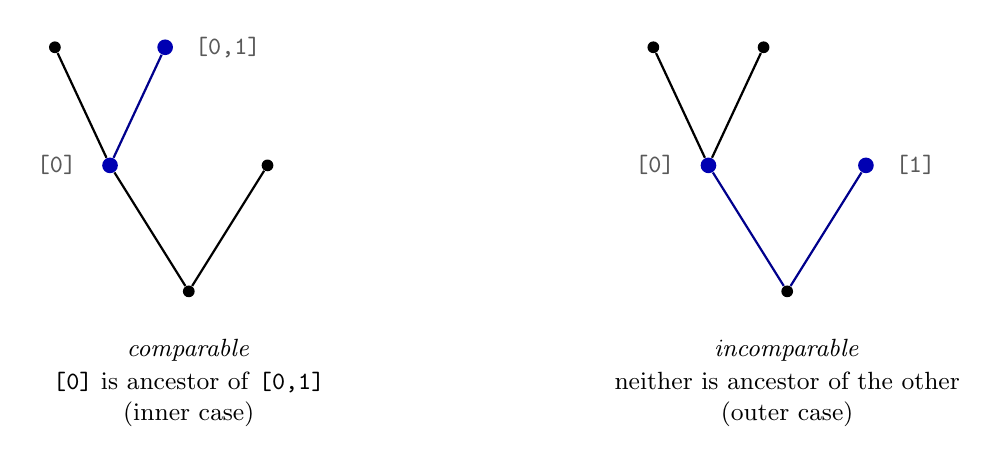
\begin{tikzpicture}[
  nd/.style={circle,fill=black,inner sep=1.5pt},
  hd/.style={circle,fill=blue!70!black,inner sep=2pt},
  ed/.style={thick},
  he/.style={thick,blue!55!black},
  ad/.style={font=\small\ttfamily,color=gray!70!black}
]
%--- left: comparable, [0] is ancestor of [0,1] ---
\begin{scope}[xshift=-3.8cm]
  \node[nd] (r) at (0,0){};
  \node[hd] (a) at (-1,1.6){};
  \node[nd] (b) at (-1.7,3.1){};
  \node[hd] (c) at (-0.3,3.1){};
  \node[nd] (d) at (1,1.6){};
  \draw[ed](r)--(a); \draw[ed](r)--(d);
  \draw[ed](a)--(b); \draw[he](a)--(c);
  \node[ad,left=2mm of a]{\texttt{[0]}};
  \node[ad,right=1.5mm of c]{\texttt{[0,1]}};
  \node[below=4mm of r,font=\small,align=center]
    {\emph{comparable}\\[1pt]\texttt{[0]} is ancestor of \texttt{[0,1]}\\(inner case)};
\end{scope}
%--- right: incomparable, [0] and [1] ---
\begin{scope}[xshift=3.8cm]
  \node[nd] (r) at (0,0){};
  \node[hd] (a) at (-1,1.6){};
  \node[nd] (b) at (-1.7,3.1){};
  \node[nd] (c) at (-0.3,3.1){};
  \node[hd] (d) at (1,1.6){};
  \draw[he](r)--(a); \draw[he](r)--(d);
  \draw[ed](a)--(b); \draw[ed](a)--(c);
  \node[ad,left=2mm of a]{\texttt{[0]}};
  \node[ad,right=1.5mm of d]{\texttt{[1]}};
  \node[below=4mm of r,font=\small,align=center]
    {\emph{incomparable}\\[1pt]neither is ancestor of the other\\(outer case)};
\end{scope}
\end{tikzpicture}
\end{center}
\noindent\small
Blue marks the pair of graft addresses under comparison.
Left: \texttt{[0,1]} extends \texttt{[0]}, so the second graft site lies
\emph{inside} the subtree rooted at the first site --- the inner (nested) case.
Right: \texttt{[0]} and \texttt{[1]} are on disjoint branches --- the outer
(incomparable-address) case, where the order of insertion can be reversed.

\begin{theorem}[Graft-pair decomposition]
Let \(a\in \operatorname{Leaf}_y(z)\) and \(b\in \operatorname{Leaf}_x(z')\)
and suppose
\[
\graftat{z}{a}{y}=z',
\qquad
\graftat{z'}{b}{x}=w.
\]
Then exactly one of the following holds:
\begin{enumerate}[label=\textup{(\roman*)}]
\item \emph{Inner case:} there exists a nonempty address
\(c\in \Addr(y)\setminus\{\langle\rangle\}\) such that
\[
b=a\cdot c.
\]
Equivalently,
\[
b\in \Addr_{z'}(a)\setminus\{a\}.
\]
If \(y'=\graftat{y}{c}{x}\), then
\[
\graftat{z'}{a\cdot c}{x}
=
\graftat{z}{a}{y'}.
\]
\item \emph{Outer case:} \(a\) and \(b\) are incomparable in the partially
ordered set \((\Addr(z'),\preceq)\), and there exists \(z_3\in \PTree\) such
that
\[
\graftat{z}{b}{x}=z_3
\qquad\text{and}\qquad
\graftat{z_3}{a}{y}=w.
\]
\end{enumerate}
\end{theorem}

\begin{proof}
Let \(a\) be the address at which \(y\) is grafted into \(z\), and let \(b\)
be the address at which \(x\) is grafted into the resulting tree \(z'\). By
the address-classification theorem formalized in
\texttt{two\_step\_graft\_decomposition\_full}, exactly one of two things can
happen.

Either \(a\prec b\). By definition of the prefix order there is a nonempty
sequence \(c\) such that \(b=a\cdot c\). Equivalently,
\[
b\in \Addr_{z'}(a)\setminus\{a\}.
\]
Thus the second graft address lies in the address cone below the root of the
inserted copy of \(y\), so the second graft is inner. If \(y'\) is obtained
from \(y\) by grafting \(x\) at \(c\), then locality of replacement at a
subtree gives
\[
\graftat{(\graftat{z}{a}{y})}{a\cdot c}{x}
=
\graftat{z}{a}{(\graftat{y}{c}{x})}.
\]
So the same output \(w\) may be read as arising from an inner graft of \(x\)
into \(y\), followed by insertion of the result into \(z\). This is the inner
case.

Or else \(a\not\preceq b\). Since the second graft is successful, the address
classification lemma excludes the possibility that \(b\prec a\). Therefore \(a\)
and \(b\) are incomparable in the partial order \((\Addr(z'),\preceq)\). By
the preceding proposition,
\[
\Addr_{z'}(a)\cap \Addr_{z'}(b)=\varnothing.
\]
Hence the two local replacements are supported on disjoint rooted subtrees of
\(z'\), and so the order of the two graft operations may be reversed without
changing the resulting proof tree. This is the outer case.

The two cases are mutually exclusive because a pair of addresses in a partial
order cannot be simultaneously comparable and incomparable.
\end{proof}

\begin{remark}
This theorem is the geometric heart of the associator analysis. It shows that
the only essential distinction among graft pairs is between the
prefix-comparable and prefix-incomparable regimes for the two graft addresses.
\end{remark}

\begin{theorem}[Commutation at incomparable addresses]
If two successful graftings occur at incomparable addresses, then performing
them in either order yields the same final proof tree.
\end{theorem}

\begin{proof}
If addresses \(a\) and \(b\) are incomparable, then neither extends the
other. Hence the subtree rooted at \(a\) and the subtree rooted at \(b\) are
disjoint. Grafting at \(a\) replaces only the subtree at \(a\), so it leaves
the subtree at \(b\) unchanged; similarly, grafting at \(b\) leaves the
subtree at \(a\) unchanged.

Therefore the two local replacement operations commute:
\[
\graftat{(\graftat{z}{a}{y})}{b}{x}
=
\graftat{(\graftat{z}{b}{x})}{a}{y}.
\]
Whenever both successive graftings are defined, they yield the same final proof
tree.
\end{proof}



\section{Algebraic preliminaries}

We now recall the standard algebraic notion to which the proof-theoretic
analysis will later lead.

\subsection{Linear, forest, and enveloping carriers}

There are three algebraic carriers in the background, and it is important not
to conflate them.

\begin{definition}[Linear span of proof trees]
Let
\[
V:=\ZZ\langle\PTree\rangle
\]
be the free abelian group on proof trees. Its basis elements are denoted
\(e_t\), for \(t\in\PTree\). The grafting product
\(\triangleright\) is a bilinear operation on \(V\). It is not a forest
product: it is proof composition by matching-leaf substitution.
\end{definition}

\begin{definition}[Forests]
A \emph{proof forest} is a finite commutative product of proof trees. We write
\[
\Forest(\PTree)
\]
for the free commutative monoid on \(\PTree\). Its unit is the empty forest,
denoted \(1\). The free commutative algebra on proof trees is
\[
\ZZ[\Forest(\PTree)]\cong S_{\ZZ}(V),
\]
the symmetric algebra on the free module \(V\). Multiplication in this algebra
is disjoint union of forests.
\end{definition}

\begin{remark}
The forest product is mathematically standard in Connes--Kreimer and
Grossman--Larson style Hopf algebras on rooted trees. Proof-theoretically,
however, a forest is not itself a single derivation. It is a formal commutative
product of derivations. This is why the proof-composition operation in the
present paper is grafting, while the Hopf-algebraic unit naturally appears
only after passing to a forest or enveloping-algebra carrier.
\end{remark}

\begin{definition}[Weight grading]
The \emph{weight} of a proof tree is its number of vertices:
\[
|t|:=|V_t|.
\]
The weight of a forest is additive:
\[
|t_1\cdots t_k|:=|t_1|+\cdots+|t_k|,
\qquad |1|:=0.
\]
This gives gradings
\[
V=\bigoplus_{n\ge 1}V_n,
\qquad
\ZZ[\Forest(\PTree)]=\bigoplus_{n\ge 0}H_n,
\]
where \(V_n\) is generated by trees of weight \(n\), and \(H_n\) by forests of
total weight \(n\).
\end{definition}

\begin{proposition}[Weight of grafting]
If \(w\in\Graft(x,y)\), then
\[
|w|=|x|+|y|-1.
\]
Equivalently, if one uses the reduced weight
\(\|t\|:=|t|-1\), then
\[
\|w\|=\|x\|+\|y\|.
\]
\end{proposition}

\begin{proof}
Grafting \(x\) into \(y\) at a leaf replaces one vertex of \(y\), namely the
matched leaf, by the whole tree \(x\). Thus the resulting vertex set is the
disjoint union of the vertices of \(y\) not equal to the grafted leaf together
with the vertices of \(x\). Hence
\[
|w|=(|y|-1)+|x|.
\]
The reduced-weight formula follows by subtracting \(1\) from both sides.
\end{proof}

\begin{remark}
The reduced weight is the grading naturally compatible with proof
composition, while the unreduced weight is the grading naturally used in
ordinary rooted-tree Hopf algebras. This small shift is harmless, but making it
explicit prevents confusion when comparing with the Connes--Kreimer and
Foissy conventions.
\end{remark}

\begin{definition}[Enveloping carrier]
If \(V\) carries a right pre-Lie product \(\triangleright\), then its
commutator
\[
[x,y]:=x\triangleright y-y\triangleright x
\]
is a Lie bracket. We write \(U(V_{\mathrm{Lie}})\) for the universal
enveloping algebra of the resulting Lie algebra. By the
Poincare--Birkhoff--Witt theorem, \(U(V_{\mathrm{Lie}})\) has an associated
graded algebra isomorphic to the symmetric algebra \(S_{\ZZ}(V)\).
\end{definition}

\begin{remark}[Oudom--Guin perspective]
The Oudom--Guin construction starts from a pre-Lie algebra and builds an
associative product on the symmetric algebra \(S(V)\) whose induced Hopf
algebra is canonically isomorphic to \(U(V_{\mathrm{Lie}})\). In this route,
the coproduct is the standard primitive-generator coproduct:
\[
\Delta(x)=x\otimes 1+1\otimes x
\qquad (x\in V),
\]
extended multiplicatively to \(S(V)\). This is different from the
Connes--Kreimer cut coproduct, whose definition is by admissible cuts of
rooted trees. One of the mathematical tasks of the present project is to
understand how these two coproduct viewpoints interact for proof trees.
\end{remark}

\subsection{Pre-Lie algebras}

\begin{definition}
A \emph{right pre-Lie algebra} over \(\ZZ\) is an abelian group \(A\) equipped
with a bilinear product \(\triangleright\) satisfying
\[
(x\triangleright y)\triangleright z - x\triangleright (y\triangleright z)
=
(x\triangleright z)\triangleright y - x\triangleright (z\triangleright y)
\]
for all \(x,y,z\in A\).
\end{definition}

\begin{remark}
Every right pre-Lie algebra carries an induced Lie bracket
\[
[x,y] := x\triangleright y - y\triangleright x.
\]
The present paper does not yet construct the full enveloping Hopf algebra from
this bracket. Instead, it establishes the quotient-controlled proof-theoretic
pre-Lie identity that would supply the input for such a construction.

\medskip
\noindent\textit{Why quotienting is necessary.}
One might hope to verify the pre-Lie identity directly at the level of
raw proof trees, by tracking explicit address data.  This fails for a
structural reason: a single term $x\triangleright(y\triangleright z)$ can be
\emph{witnessed} by many distinct ordered pairs of graft addresses, depending on
which matching leaf of $y\triangleright z$ is chosen for the outer step. These
witnesses encode the same geometric configuration --- the same insertion event
at the same relative position in the tree --- but differ in the raw list entry
that records it.  Any equation between graft pairs is therefore really an
equation between \emph{equivalence classes} of address records, not between the
records themselves.

More precisely, two witnesses are \emph{bureaucratically equivalent}
if they agree on which insertion is nested inside which, and whether the
outer insertions act on disjoint branches or on ancestor-descendant
pairs.  The quotient by this equivalence retains exactly the dependency
geometry and discards all bookkeeping accidents.  The pre-Lie identity
\[
(x\triangleright y)\triangleright z - x\triangleright(y\triangleright z)
=
(x\triangleright z)\triangleright y - x\triangleright(z\triangleright y)
\]
holds in this quotient: the left-hand side and the right-hand side
collect the \emph{same} noise classes with opposite signs (those
cancel) and the same residual classes (those match term for term).
Without the quotient, the witness sets on the two sides of the equation
are not equal as sets of address records, only equal in cardinality
after noise removal; the quotient is what supplies the required
bijection.

For fixed \(x,y,z,w\), let \(\mathcal W_L(x,y,z;w)\) be the set of successful
ordered pairs of graftings contributing to the coefficient of \(w\) in
\((x\triangleright y)\triangleright z - x\triangleright(y\triangleright z)\),
and let \(\mathcal W_R(x,y,z;w)\) be the analogous set for the swapped
expression
\((y\triangleright x)\triangleright z - y\triangleright(x\triangleright z)\).
Then the raw pre-Lie identity would amount to a sign-preserving bijection
between \(\mathcal W_L(x,y,z;w)\) and \(\mathcal W_R(x,y,z;w)\) for every
output tree \(w\). What the formal development shows is subtler: there is in
general no canonical bijection at raw witness level, but there is a canonical
comparison after passing to quotient classes of witnesses. On those quotient
classes, the noise sector cancels and the residual sector is matched
bijectionally.
\end{remark}

\begin{theorem}[Oudom--Guin extension theorem]
Let \((A,\triangleright)\) be a right pre-Lie algebra over a commutative
ground ring. Then the symmetric algebra \(S(A)\) carries an associative product
\(\star\), extending the pre-Lie operation, for which \(S(A)\) becomes a Hopf
algebra with coproduct determined by declaring every \(a\in A\) primitive:
\[
\Delta(a)=a\otimes 1+1\otimes a.
\]
Equivalently, this Hopf algebra is canonically isomorphic to the universal
enveloping algebra of the Lie algebra \(A_{\mathrm{Lie}}\) induced by the
commutator of \(\triangleright\).
\end{theorem}

\begin{proof}[Idea of construction]
The pre-Lie product defines derivations of the symmetric algebra by insertion.
One recursively extends the action of \(A\) on \(S(A)\), then defines
\(\star\) by letting the left tensor factor act on the right one. The pre-Lie
identity is exactly the compatibility condition needed for associativity. The
primitive coproduct is the usual symmetric-algebra coproduct, and the
associative product is compatible with it; this yields the Hopf algebra. The
commutator Lie algebra comparison is the Oudom--Guin identification with the
universal enveloping algebra.
\end{proof}

\begin{remark}
Thus, once the proof-tree grafting product has descended to a genuine pre-Lie
product on the intended quotient carrier, the Hopf algebra is not an additional
ad hoc construction. It is supplied functorially by the Oudom--Guin theorem.
The remaining proof-theoretic burden is to identify the correct carrier and
prove descent of the grafting product to it.
\end{remark}



\section{Quotienting bureaucratic graft-pair data}

At raw address level, graft-pair configurations still contain too much
presentation data. The next step is to isolate their genuine dependency
geometry.

\subsection{Associator witnesses as ordered graft pairs}

\begin{definition}
Fix proof trees \(x,y,z,w\). A \emph{left witness for \(w\)} is a successful
ordered pair of grafting operations contributing to the left-bracketed
associator. Concretely, it is one of the following two kinds of data.
\begin{enumerate}[label=\textup{(\roman*)}]
\item \emph{Outer witness:} addresses \(a,b\) and an intermediate tree \(z'\)
such that grafting \(y\) into \(z\) at address \(a\) yields \(z'\), and then
grafting \(x\) into \(z'\) at address \(b\) yields \(w\):
\[
\graftat{z}{a}{y}=z',
\qquad
\graftat{z'}{b}{x}=w.
\]
\item \emph{Inner witness:} an internal address \(c\) in \(x\), an address
\(a\) in \(z\), and an intermediate tree \(u\) such that grafting \(y\) into
\(x\) at address \(c\) yields \(u\), and then grafting \(u\) into \(z\) at
address \(a\) yields \(w\):
\[
\graftat{x}{c}{y}=u,
\qquad
\graftat{z}{a}{u}=w.
\]
\end{enumerate}
\noindent
A \emph{swapped-right witness for \(w\)} is defined analogously:
\begin{enumerate}[label=\textup{(\roman*)}]
\item \emph{Outer witness:} addresses \(a,b\) and an intermediate tree \(z'\)
such that
\[
\graftat{z}{a}{x}=z',
\qquad
\graftat{z'}{b}{y}=w.
\]
\item \emph{Inner witness:} an internal address \(c\) in \(y\), an address
\(a\) in \(z\), and an intermediate tree \(u\) such that
\[
\graftat{y}{c}{x}=u,
\qquad
\graftat{z}{a}{u}=w.
\]
\end{enumerate}
\end{definition}

\begin{definition}[Witness sets]
For fixed \(x,y,z,w\), let \(W^{\mathrm{out}}_L(x,y,z;w)\) be the set of all
triples \((a,b,z')\in \mathbb N^{<\omega}\times \mathbb N^{<\omega}\times \PTree\)
such that \(a\in \Addr(z)\), \(b\in \Addr(z')\), and
\[
\graftat{z}{a}{y}=z',
\qquad
\graftat{z'}{b}{x}=w.
\]
Let \(W^{\mathrm{in}}_L(x,y,z;w)\) be the set of all tuples
\((c,a,u)\in \mathbb N^{<\omega}\times \mathbb N^{<\omega}\times \PTree\) such
that \(c\in \Addr(x)\), \(a\in \Addr(z)\), and
\[
\graftat{x}{c}{y}=u,
\qquad
\graftat{z}{a}{u}=w.
\]
\[
W^{\mathrm{out}}_R(x,y,z;w):=
\{(a,b,z')\in \mathbb N^{<\omega}\times \mathbb N^{<\omega}\times \PTree
 \mid a\in \Addr(z),\ b\in \Addr(z'),\
 \graftat{z}{a}{x}=z',\ \graftat{z'}{b}{y}=w\},
\]
\[
W^{\mathrm{in}}_R(x,y,z;w):=
\{(c,a,u)\in \mathbb N^{<\omega}\times \mathbb N^{<\omega}\times \PTree
 \mid c\in \Addr(y),\ a\in \Addr(z),\
 \graftat{y}{c}{x}=u,\ \graftat{z}{a}{u}=w\}.
\]
The full left and swapped-right witness fibres are
\[
W_L(x,y,z;w):=W^{\mathrm{out}}_L(x,y,z;w)\cup W^{\mathrm{in}}_L(x,y,z;w).
\]
\[
W_R(x,y,z;w):=W^{\mathrm{out}}_R(x,y,z;w)\cup W^{\mathrm{in}}_R(x,y,z;w).
\]
\end{definition}

\begin{remark}[Set-theoretic form of the two-step dichotomy]
The graft-pair decomposition theorem proved earlier implies that every
successful ordered pair of grafts contributing to the left bracketing belongs
to exactly one of the two fibres \(W^{\mathrm{out}}_L(x,y,z;w)\) or
\(W^{\mathrm{in}}_L(x,y,z;w)\); likewise, every successful ordered pair
contributing to the swapped-right bracketing belongs to exactly one of
\(W^{\mathrm{out}}_R(x,y,z;w)\) or \(W^{\mathrm{in}}_R(x,y,z;w)\). Thus the
outer/inner distinction is defined before quotienting; the quotient is used
only to identify different presentations of the same two-step geometry.
\end{remark}

\subsection{Graft-pair classes}

\begin{definition}[Tagged raw code fibres]
For fixed \(x,y,z,w\), define
\[
\mathrm{Code}(x,y,z;w):=
\bigl(\{\mathsf{Lout}\}\times W^{\mathrm{out}}_L(x,y,z;w)\bigr)
\sqcup
\bigl(\{\mathsf{Lin}\}\times W^{\mathrm{in}}_L(x,y,z;w)\bigr)
\]
\[
\sqcup
\bigl(\{\mathsf{Rout}\}\times W^{\mathrm{out}}_R(x,y,z;w)\bigr)
\sqcup
\bigl(\{\mathsf{Rin}\}\times W^{\mathrm{in}}_R(x,y,z;w)\bigr).
\]
We write the corresponding tagged elements as
\[
\mathsf{Lout}(a,b,z'),\qquad
\mathsf{Lin}(c,a,u),\qquad
\mathsf{Rout}(a,b,z'),\qquad
\mathsf{Rin}(c,a,u).
\]
\end{definition}

\begin{definition}[Generator relations]
Fix \(x,y,z,w\). The four basic comparison relations on
\(\mathrm{Code}(x,y,z;w)\) are the following subsets of
\(\mathrm{Code}(x,y,z;w)\times \mathrm{Code}(x,y,z;w)\).
\begin{enumerate}[label=\textup{(\roman*)}]
\item \(R_{\mathrm{oo}}\) consists of all pairs
\[
\bigl(\mathsf{Lout}(a,b,z'),\mathsf{Rout}(b,a,z_3)\bigr)
\]
such that \((a,b,z')\in W^{\mathrm{out}}_L(x,y,z;w)\), both \(a\) and \(b\)
belong to \(\Addr(z)\), \(a\) and \(b\) are incomparable in
\((\Addr(z),\preceq)\), \(z_3=\graftat{z}{b}{x}\), and
\[
\graftat{z_3}{a}{y}=w.
\]
\item \(R_{\mathrm{oi}}\) consists of all pairs
\[
\bigl(\mathsf{Lout}(a,a\cdot c,z'),\mathsf{Rin}(c,a,u)\bigr)
\]
such that \((a,a\cdot c,z')\in W^{\mathrm{out}}_L(x,y,z;w)\),
\(c\neq \langle\rangle\),
\[
u=\graftat{y}{c}{x},
\qquad
\graftat{z}{a}{u}=w.
\]
\item \(R_{\mathrm{bo}}\) consists of all pairs
\[
\bigl(\mathsf{Rout}(a,b,z'),\mathsf{Lout}(b,a,z_3)\bigr)
\]
such that \((a,b,z')\in W^{\mathrm{out}}_R(x,y,z;w)\), both \(a\) and \(b\)
belong to \(\Addr(z)\), \(a\) and \(b\) are incomparable in
\((\Addr(z),\preceq)\), \(z_3=\graftat{z}{b}{y}\), and
\[
\graftat{z_3}{a}{x}=w.
\]
\item \(R_{\mathrm{bi}}\) consists of all pairs
\[
\bigl(\mathsf{Rout}(a,a\cdot c,z'),\mathsf{Lin}(c,a,u)\bigr)
\]
such that \((a,a\cdot c,z')\in W^{\mathrm{out}}_R(x,y,z;w)\),
\(c\neq \langle\rangle\),
\[
u=\graftat{x}{c}{y},
\qquad
\graftat{z}{a}{u}=w.
\]
\end{enumerate}
\end{definition}

\begin{definition}[Bureaucratic equivalence]
The \emph{bureaucratic equivalence relation}
\[
\sim_{\mathrm b}\ \subseteq\ \mathrm{Code}(x,y,z;w)\times \mathrm{Code}(x,y,z;w)
\]
is the least equivalence relation containing the four generator relations
\[
R_{\mathrm{oo}},\qquad
R_{\mathrm{oi}},\qquad
R_{\mathrm{bo}},\qquad
R_{\mathrm{bi}}.
\]
\end{definition}

\begin{proposition}[Bureaucratic equivalence preserves the composite tree]
Let \(\xi,\eta\in \mathrm{Code}(x,y,z;w)\).
\begin{enumerate}[label=\textup{(\roman*)}]
\item If \((\xi,\eta)\in R_{\mathrm{oo}}\cup R_{\mathrm{oi}}\cup
R_{\mathrm{bo}}\cup R_{\mathrm{bi}}\), then \(\xi\) and \(\eta\) determine the
same terminal proof tree \(w\).
\item If \(\xi\sim_{\mathrm b}\eta\), then \(\xi\) and \(\eta\) represent the
same class in the quotient \(\mathrm{Code}(x,y,z;w)/{\sim_{\mathrm b}}\).
\end{enumerate}
\end{proposition}

\begin{proof}
For \textup{(i)}, suppose first that
\[
\bigl(\mathsf{Lout}(a,b,z'),\mathsf{Rout}(b,a,z_3)\bigr)\in R_{\mathrm{oo}}.
\]
Then
\[
\graftat{z}{a}{y}=z',
\qquad
\graftat{z'}{b}{x}=w,
\qquad
\graftat{z}{b}{x}=z_3,
\]
and \(a,b\in \Addr(z)\) are incomparable. By the commutation theorem for
graftings at incomparable addresses,
\[
\graftat{z_3}{a}{y}=w.
\]
Hence the two tagged codes lie in the same fibre and have the same output.

Suppose next that
\[
\bigl(\mathsf{Lout}(a,a\cdot c,z'),\mathsf{Rin}(c,a,u)\bigr)\in R_{\mathrm{oi}}.
\]
Then
\[
\graftat{z}{a}{y}=z',
\qquad
\graftat{z'}{a\cdot c}{x}=w,
\qquad
u=\graftat{y}{c}{x},
\qquad
\graftat{z}{a}{u}=w.
\]
Moreover,
\[
\graftat{z'}{a\cdot c}{x}
\;=\;
\graftat{\graftat{z}{a}{y}}{a\cdot c}{x}
\;=\;
\graftat{z}{a}{\graftat{y}{c}{x}}
\;=\;
\graftat{z}{a}{u},
\]
which is exactly the locality-of-replacement identity on the rooted subtree
inserted at address \(a\). Thus the two tagged codes again have the same
terminal tree \(w\).

The cases of \(R_{\mathrm{bo}}\) and \(R_{\mathrm{bi}}\) are the same two
arguments with \(x\) and \(y\) interchanged.

For \textup{(ii)}, equality of quotient classes is by definition the
equivalence relation \(\sim_{\mathrm b}\). Thus \(\xi\sim_{\mathrm b}\eta\)
implies
\[
[\,\xi\,]=[\,\eta\,]
\qquad\text{in}\qquad
\mathrm{Code}(x,y,z;w)/{\sim_{\mathrm b}}.
\]
\end{proof}

\begin{remark}
The quotient by \(\sim_{\mathrm b}\) is therefore a quotient of the tagged raw
code fibre \(\mathrm{Code}(x,y,z;w)\), not of the set of trees with terminal
label \(w\). Equality in the quotient is equality of equivalence classes of
two-step presentations:
\[
[\,\xi\,]=[\,\eta\,]
\quad\Longleftrightarrow\quad
\xi\sim_{\mathrm b}\eta.
\]
What is forgotten is the particular address presentation of the two-step
composite; what is retained is the quotient class of that presentation.
\end{remark}

% ---- Figure 4: the four two-step codes ----
\begin{center}
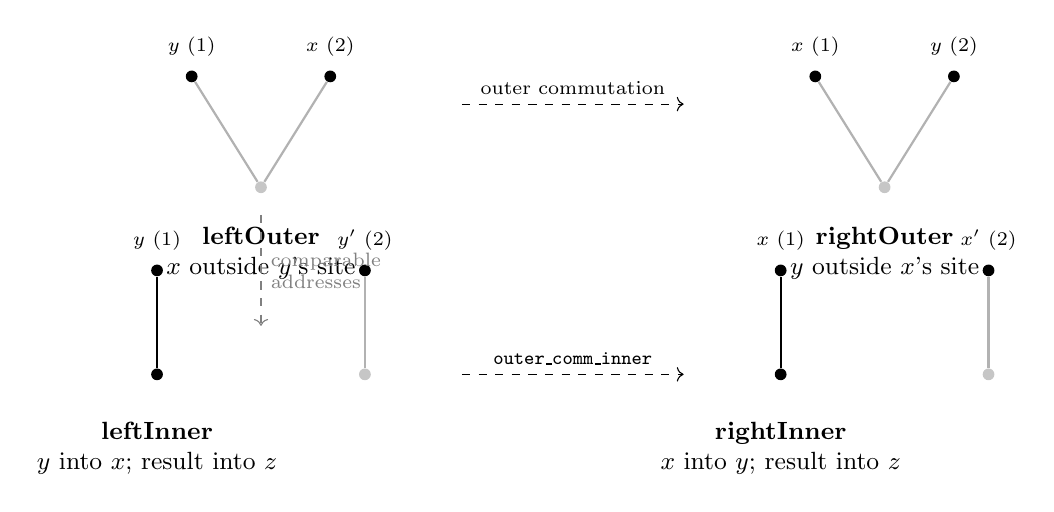
\begin{tikzpicture}[scale=0.88,
  nd/.style={circle,fill=black,inner sep=1.5pt},
  znd/.style={circle,fill=gray!45,inner sep=1.5pt},
  ed/.style={thick},
  ze/.style={thick,gray!60},
  lb/.style={font=\small}
]
% ---- top row: outer cases (both grafts act on z or its modification) ----
% leftOuter
\begin{scope}[xshift=-4.5cm,yshift=4.2cm]
  \node[znd] (z)  at (0,0)    {};
  \node[nd]  (a)  at (-1,1.6) {};
  \node[nd]  (b)  at (1,1.6)  {};
  \draw[ze](z)--(a); \draw[ze](z)--(b);
  \node[above=0.5mm of a,font=\scriptsize]{$y$ (1)};
  \node[above=0.5mm of b,font=\scriptsize]{$x$ (2)};
  \node[lb,below=3mm of z,align=center]{\textbf{leftOuter}\\$x$ outside $y$'s site};
\end{scope}
% rightOuter
\begin{scope}[xshift=4.5cm,yshift=4.2cm]
  \node[znd] (z)  at (0,0)    {};
  \node[nd]  (a)  at (-1,1.6) {};
  \node[nd]  (b)  at (1,1.6)  {};
  \draw[ze](z)--(a); \draw[ze](z)--(b);
  \node[above=0.5mm of a,font=\scriptsize]{$x$ (1)};
  \node[above=0.5mm of b,font=\scriptsize]{$y$ (2)};
  \node[lb,below=3mm of z,align=center]{\textbf{rightOuter}\\$y$ outside $x$'s site};
\end{scope}
% dashed equivalence arrow top
\draw[dashed,->] (-1.6,5.4) -- (1.6,5.4)
  node[midway,above,font=\scriptsize]{outer commutation};
% ---- bottom row: inner cases (one tree grafted into another first) ----
% leftInner
\begin{scope}[xshift=-4.5cm,yshift=0cm]
  \node[nd]  (x)  at (-1.5,1.5) {};
  \node[nd]  (ya) at (-1.5,3.0) {};
  \node[znd] (z)  at (1.5,1.5)  {};
  \node[nd]  (zb) at (1.5,3.0)  {};
  \draw[ed](x)--(ya); \draw[ze](z)--(zb);
  \node[above=0.5mm of ya,font=\scriptsize]{$y$ (1)};
  \node[above=0.5mm of zb,font=\scriptsize]{$y'$ (2)};
  \node[lb,below=4mm of x,align=center]{\textbf{leftInner}\\$y$ into $x$; result into $z$};
\end{scope}
% rightInner
\begin{scope}[xshift=4.5cm,yshift=0cm]
  \node[nd]  (y)  at (-1.5,1.5) {};
  \node[nd]  (xa) at (-1.5,3.0) {};
  \node[znd] (z)  at (1.5,1.5)  {};
  \node[nd]  (zb) at (1.5,3.0)  {};
  \draw[ed](y)--(xa); \draw[ze](z)--(zb);
  \node[above=0.5mm of xa,font=\scriptsize]{$x$ (1)};
  \node[above=0.5mm of zb,font=\scriptsize]{$x'$ (2)};
  \node[lb,below=4mm of y,align=center]{\textbf{rightInner}\\$x$ into $y$; result into $z$};
\end{scope}
% dashed equivalence arrow bottom
\draw[dashed,->] (-1.6,1.5) -- (1.6,1.5)
  node[midway,above,font=\scriptsize]{\texttt{outer\_comm\_inner}};
% vertical: leftOuter ~ rightInner at comparable addresses
\draw[dashed,->,gray] (-4.5,3.8) -- (-4.5,2.2)
  node[midway,right,font=\scriptsize,gray,align=left]{comparable\\addresses};
\end{tikzpicture}
\end{center}
\noindent\small
This figure is schematic. Its four labelled positions represent the four tagged
components \(\mathsf{Lout}\), \(\mathsf{Lin}\), \(\mathsf{Rout}\),
\(\mathsf{Rin}\) of the fibre \(\mathrm{Code}(x,y,z;w)\). The upper dashed
arrow represents the relation \(R_{\mathrm{oo}}\subseteq
\mathsf{Lout}\times\mathsf{Rout}\), defined on incomparable address pairs in
\(\Addr(z)\). The comparable-address transport is the relation
\(R_{\mathrm{oi}}\subseteq \mathsf{Lout}\times\mathsf{Rin}\), defined on tuples
of the form \((a,a\cdot c,z')\). The converse relations are
\(R_{\mathrm{bo}}\subseteq \mathsf{Rout}\times\mathsf{Lout}\) and
\(R_{\mathrm{bi}}\subseteq \mathsf{Rout}\times\mathsf{Lin}\). Grey vertices
belong to the receiver tree \(z\); black vertices indicate the address
components occurring in the corresponding raw code tuples.

\begin{proposition}[Comparable-address criterion for the mixed generator]
Let
\[
\xi=\mathsf{Lout}(a,b,z')\in \mathrm{Code}(x,y,z;w).
\]
Then there exists \(\eta\in \mathrm{Code}(x,y,z;w)\) such that
\[
(\xi,\eta)\in R_{\mathrm{oi}}
\]
if and only if there exists an address \(c\in \mathbb N^{<\omega}\) with
\[
b=a\cdot c.
\]
Whenever this holds, every such \(\eta\) has the form
\[
\eta=\mathsf{Rin}(c,a,u)
\]
for a tree \(u\) satisfying
\[
u=\graftat{y}{c}{x},
\qquad
\graftat{z}{a}{u}=w.
\]
\end{proposition}

\begin{proof}
If \((\xi,\eta)\in R_{\mathrm{oi}}\), then by definition of \(R_{\mathrm{oi}}\)
\(\xi\) must be of the form \(\mathsf{Lout}(a,a\cdot c,z')\) for some
\(c\in \mathbb N^{<\omega}\). Thus \(b=a\cdot c\).

Conversely, suppose \(b=a\cdot c\). If
\[
\xi=\mathsf{Lout}(a,a\cdot c,z')
\]
lies in \(\mathrm{Code}(x,y,z;w)\), then
\[
\graftat{z}{a}{y}=z',
\qquad
\graftat{z'}{a\cdot c}{x}=w.
\]
Set \(u:=\graftat{y}{c}{x}\). By locality of replacement on the rooted subtree
inserted at \(a\),
\[
\graftat{z}{a}{u}
\;=\;
\graftat{z}{a}{\graftat{y}{c}{x}}
\;=\;
\graftat{\graftat{z}{a}{y}}{a\cdot c}{x}
\;=\;
\graftat{z'}{a\cdot c}{x}
\;=\;
w.
\]
Therefore
\[
\eta:=\mathsf{Rin}(c,a,u)
\]
satisfies \((\xi,\eta)\in R_{\mathrm{oi}}\). The final statement is again just
the defining form of \(R_{\mathrm{oi}}\).
\end{proof}

\begin{proposition}[Identity of two-step proof compositions]
For \(c,d\in \mathrm{Code}(x,y,z;w)\),
\[
[c]=[d]\ \text{in}\ \mathrm{Code}(x,y,z;w)/{\sim_{\mathrm b}}
\]
if and only if there exists a finite chain
\[
c=c_0,\ c_1,\ \dots,\ c_n=d
\]
of raw graft-pair codes in \(\mathrm{Code}(x,y,z;w)\) such that, for each
\(i<n\), the pair \((c_i,c_{i+1})\) is related by one generating move of the
bureaucratic equivalence relation, that is, belongs to
\[
R_{\mathrm{oo}}\cup R_{\mathrm{oi}}\cup R_{\mathrm{bo}}\cup R_{\mathrm{bi}}
\]
or to the converse of one of these four relations.
\end{proposition}

\begin{proof}
By definition, \(\Qclass(x,y,z;w)\) is the quotient of
\(\mathrm{Code}(x,y,z;w)\) by the equivalence relation \(\sim_{\mathrm b}\)
generated by the four relations
\[
R_{\mathrm{oo}},\qquad
R_{\mathrm{oi}},\qquad
R_{\mathrm{bo}},\qquad
R_{\mathrm{bi}}.
\]
Hence
\([c]=[d]\) is equivalent to \(c\sim_{\mathrm b} d\). Since
\(\sim_{\mathrm b}\) is the least equivalence relation containing those
four relations, the statement \(c\sim_{\mathrm b} d\) is in turn equivalent
to the existence of a finite zig-zag from \(c\) to \(d\) built from generators
and their converses. This is exactly the required chain description.
\end{proof}

\begin{definition}
The quotient set of graft-pair codes is denoted
\[
\Qclass(x,y,z;w).
\]
More formally, if \(\mathrm{Code}(x,y,z;w)\) denotes the set of all raw
graft-pair codes with output \(w\), and if \(\sim_{\mathrm{b}}\) is the
bureaucratic equivalence relation, then
\[
\Qclass(x,y,z;w):=\mathrm{Code}(x,y,z;w)/{\sim_{\mathrm{b}}}.
\]
Inside it we distinguish the left contribution classes
\[
\CL(x,y,z;w)
\]
and the swapped-right contribution classes
\[
\CR(x,y,z;w),
\]
the latter being associated with the swapped bracketing \((y,x,z)\).
\end{definition}

\begin{definition}[Quotient projection]
The quotient map
\[
\pi_{x,y,z;w} :
\mathrm{Code}(x,y,z;w)
\twoheadrightarrow
\Qclass(x,y,z;w)
\]
sends a raw graft-pair code \(c\) to its bureaucratic equivalence class
\([c]\). In particular, the left and swapped-right contribution classes are
images under \(\pi_{x,y,z;w}\) of the corresponding subsets of raw left and raw
swapped-right witnesses.
\end{definition}

\begin{definition}[Classwise comparison relation]
The relation
\[
\Swap_{x,y,z;w}\subseteq \Qclass(x,y,z;w)\times \Qclass(y,x,z;w)
\]
is defined by declaring \(([c],[d])\in \Swap_{x,y,z;w}\) when there exist raw
representatives
\[
\xi\in \mathrm{Code}(x,y,z;w),
\qquad
\eta\in \mathrm{Code}(y,x,z;w)
\]
with
\[
\pi_{x,y,z;w}(\xi)=[c],
\qquad
\pi_{y,x,z;w}(\eta)=[d],
\]
such that the ordered pair \((\xi,\eta)\) lies in the graph of one of the four
generator relations after swapping the parameters \((x,y)\leftrightarrow(y,x)\).
Equivalently, \(\Swap_{x,y,z;w}\) is the quotient image of the union of the
four generator relations under the two quotient maps. Because these relations
are compatible with \(\sim_{\mathrm b}\), \(\Swap_{x,y,z;w}\) is well-defined.
\end{definition}

\begin{remark}
An element of \(\CL(x,y,z;w)\) or \(\CR(x,y,z;w)\) should therefore be read as
an equivalence class of \emph{pairs of grafting operations} with output \(w\),
not as a single derivation history. The quotient identifies histories that
differ only by bureaucratic scheduling, or by two equivalent descriptions of
the same nested dependency. This is the formal counterpart of the
proof-theoretic principle that identity of proof should ignore inessential
orderings of operations supported at incomparable addresses while retaining
genuine dependency.
\end{remark}

\begin{definition}[Support predicates and sector decomposition on the left carrier]
Fix \(x,y,z,w\), and let \(q\in \CL(x,y,z;w)\).
\begin{enumerate}[label=\textup{(\roman*)}]
\item \(q\) has \emph{left outer support} if it admits a representative in
\(W^{\mathrm{out}}_L(x,y,z;w)\).
\item \(q\) has \emph{left inner support} if it admits a representative in
\(W^{\mathrm{in}}_L(x,y,z;w)\).
\item \(q\) has \emph{right outer support} if there exists
\(q'\in \CR(x,y,z;w)\) such that \((q,q')\in \Swap_{x,y,z;w}\) and \(q'\) admits
a representative in \(W^{\mathrm{out}}_R(x,y,z;w)\).
\item \(q\) has \emph{right inner support} if there exists
\(q'\in \CR(x,y,z;w)\) such that \((q,q')\in \Swap_{x,y,z;w}\) and \(q'\) admits
a representative in \(W^{\mathrm{in}}_R(x,y,z;w)\).
\end{enumerate}
The two quotient-trivial noise sectors on the left carrier are then
\[
\Noise_{L\to R}(x,y,z;w)
:=
\{\,q\in \CL(x,y,z;w)\mid
\text{$q$ has left outer support and right inner support}\,\},
\]
\[
\Noise_{R\to L}(x,y,z;w)
:=
\{\,q\in \CL(x,y,z;w)\mid
\text{$q$ has right outer support and left inner support}\,\}.
\]
The \emph{residual left sector} is
\[
\Res_L(x,y,z;w)
:=
\CL(x,y,z;w)\setminus
\bigl(\Noise_{L\to R}(x,y,z;w)\cup \Noise_{R\to L}(x,y,z;w)\bigr).
\]
Finally, for \(q\in \Res_L(x,y,z;w)\), define
\[
q\in \PureOut_L(x,y,z;w)
\iff
\text{$q$ has left outer support and not left inner support},
\]
\[
q\in \PureIn_L(x,y,z;w)
\iff
\text{$q$ has left inner support and not left outer support},
\]
\[
q\in \mathsf{Mixed}_L(x,y,z;w)
\iff
\text{$q$ has both left outer and left inner support}.
\]
\end{definition}

\begin{remark}[Mathematical form of the quotient-level comparison]
For fixed \(x,y,z,w\), the class-level pre-Lie comparison problem is the
comparison of the two quotient carriers \(\CL(x,y,z;w)\) and
\(\CR(x,y,z;w)\) through the transport relation \(\Swap_{x,y,z;w}\). On the
left carrier, the quotient-trivial part is exactly
\[
\Noise_{L\to R}(x,y,z;w)\cup \Noise_{R\to L}(x,y,z;w),
\]
while the nontrivial part is the residual set \(\Res_L(x,y,z;w)\). The later
theorems prove:
\begin{enumerate}[label=\textup{(\roman*)}]
\item every residual left class belongs to exactly one of the three sectors
\(\PureOut_L(x,y,z;w)\), \(\PureIn_L(x,y,z;w)\), \(\mathsf{Mixed}_L(x,y,z;w)\);
\item the mixed residual sector \(\mathsf{Mixed}_L(x,y,z;w)\) is empty;
\item the outer and inner transport maps induce unique partners for classes in
\(\PureOut_L(x,y,z;w)\) and \(\PureIn_L(x,y,z;w)\), respectively.
\end{enumerate}
Thus the class-level associator comparison reduces to equality on the
quotient-trivial noise sector and to unique transport on the two pure residual
sectors.
\end{remark}

\subsection{Canonical transport theorems}

\begin{theorem}[Outer transport]
For every \(x,y,z,w\), outer left contribution classes are canonically in
bijection with outer contribution classes on the swapped right side.
\end{theorem}

\begin{proof}
Take an outer left witness represented by a pair of successful grafts
\[
\graftat{z}{a}{y}=z',
\qquad
\graftat{z'}{b}{x}=w,
\]
with \(a\) and \(b\) incomparable. By commutation at incomparable addresses,
there is a unique tree \(z''\) such that
\[
\graftat{z}{b}{x}=z'',
\qquad
\graftat{z''}{a}{y}=w.
\]
This defines a swapped right-outer witness with the same output \(w\).

Because this construction is obtained by commuting the same two local
operations, it depends only on the dependency geometry of the witness and not
on the particular address record chosen inside its bureaucratic equivalence
class. Hence it descends to quotient classes and gives a map from outer left
classes to swapped right-outer classes.

Applying exactly the same commutation in the reverse direction recovers the
original witness. The two maps are therefore inverse to one another, so we
obtain a canonical bijection of outer contribution classes.
\end{proof}

\begin{theorem}[Inner transport]
For every \(x,y,z,w\), inner left contribution classes are canonically in
bijection with inner contribution classes on the swapped right side.
\end{theorem}

\begin{proof}
Take an inner left witness. By definition, it is specified by an internal
address \(c\) in \(x\), an address \(a\) in \(z\), and an intermediate tree
\(u=\graftat{x}{c}{y}\) such that
\[
\graftat{z}{a}{u}=w.
\]
Now consider the swapped parameter order \((y,x,z;w)\). Relative to that order,
the same triple \((c,a,u)\) is a right-inner witness, because the first
grafting operation is precisely
\[
\graftat{x}{c}{y}=u,
\qquad
\graftat{z}{a}{u}=w.
\]
Thus the inner transport is not a change in the underlying composite tree, but
only a change in which ordered pair \((x,y)\) is regarded as the outer
bracketing parameter. The construction preserves the terminal tree \(w\),
depends only on the raw witness data \((c,a,u)\), and is inverted by the same
reinterpretation with the parameters swapped back. Therefore it descends to a
canonical bijection between left-inner classes for \((x,y,z;w)\) and
right-inner classes for \((y,x,z;w)\).
\end{proof}

\begin{remark}
The outer transport is a strict commutation theorem. The inner transport is a
reassociation theorem. Their common role is to show that the quotient keeps the
geometric content of the graft pair while discarding the accidental
presentation details.
\end{remark}

\section{Noise, residual classes, and purity}

\subsection{Noise and residual sectors}

\begin{definition}
A left contribution class is called \emph{noise} if the apparent difference
between its outer and inner presentations is already quotient-trivial under the
comparison with the swapped side. A left contribution class is
\emph{residual} if it is not noise.
\end{definition}

\begin{remark}
``Noise'' does not mean mathematically uninteresting in itself. It means
precisely that the class contributes no genuine asymmetry to the associator
comparison, because the quotient already identifies the competing
presentations.
\end{remark}

\begin{remark}
The geometric mechanism producing noise is the following. A left-outer
contribution class becomes noise when it simultaneously admits a right-inner
presentation. By the \texttt{outer\_comm\_inner} identification in the
bureaucratic equivalence, this happens exactly when the two graft addresses
are comparable. In that case, what appears from the left bracketing as an
outer insertion of $x$ into $z'$ at an address incomparable with the first
graft site can equally be read, from the
right bracketing, as $x$ being composed into $y$ first and the result placed
into $z$. The class thus contributes equally to both sides of the pre-Lie
associator and cancels. This mechanism --- comparable addresses producing
simultaneously-outer-and-inner classes --- is what the formal development
calls \emph{left-to-right overlap noise}. The noise sector is therefore not
an arbitrary algebraic device but a precise reflection of a geometric
degeneracy in the graft addresses.
\end{remark}

\begin{definition}
A residual left contribution class is called:
\begin{itemize}
\item \emph{pure outer} if it has outer support and no inner support;
\item \emph{pure inner} if it has inner support and no outer support;
\item \emph{mixed} if it has both outer and inner support.
\end{itemize}
\end{definition}

\begin{theorem}[Elimination of mixed residual classes]
There are no mixed residual left contribution classes.
\end{theorem}

\begin{lemma}[Mixed support forces overlap noise]
Let \(q\in \CL(x,y,z;w)\). If \(q\) has both left outer support and left inner
support, then \(q\in \Noise_{L\to R}(x,y,z;w)\).
\end{lemma}

\begin{proof}
Choose a left-outer representative \(\xi\) of \(q\) and a left-inner
representative \(\eta\) of \(q\). Since \([\xi]=[\eta]\) in
\(\Qclass(x,y,z;w)\), Proposition~79 gives a finite chain of generating moves
from \(\xi\) to \(\eta\). Along such a chain, the only generator relation that
changes a left-outer code into an inner code on the swapped side is
\(R_{\mathrm{oi}}\), whose defining criterion is the comparable-address
condition \(b=a\cdot c\) with \(c\neq \langle\rangle\). Hence some outer
representative of \(q\) lies in the comparable-address regime.

By Proposition~78, such a comparable left-outer representative determines a
right-inner representative of the same quotient class. Therefore \(q\) has left
outer support and right inner support, so
\[
q\in \Noise_{L\to R}(x,y,z;w).
\]
\end{proof}

\begin{proof}
Assume toward a contradiction that \(q\) is a mixed residual left
contribution class. By definition of mixedness, \(q\) has both left outer
support and left inner support. By the preceding lemma,
\[
q\in \Noise_{L\to R}(x,y,z;w).
\]
But \(q\) was assumed residual, so by definition
\[
q\notin \Noise_{L\to R}(x,y,z;w)\cup \Noise_{R\to L}(x,y,z;w),
\]
a contradiction. Therefore no mixed residual left contribution class exists.
\end{proof}

\begin{corollary}[Residual purity]
Every residual left contribution class is either pure outer or pure inner.
\end{corollary}

\begin{proof}
By the theorem, the mixed case is impossible.
\end{proof}

% ---- Figure 6: the noise/residual trichotomy ----
\begin{center}
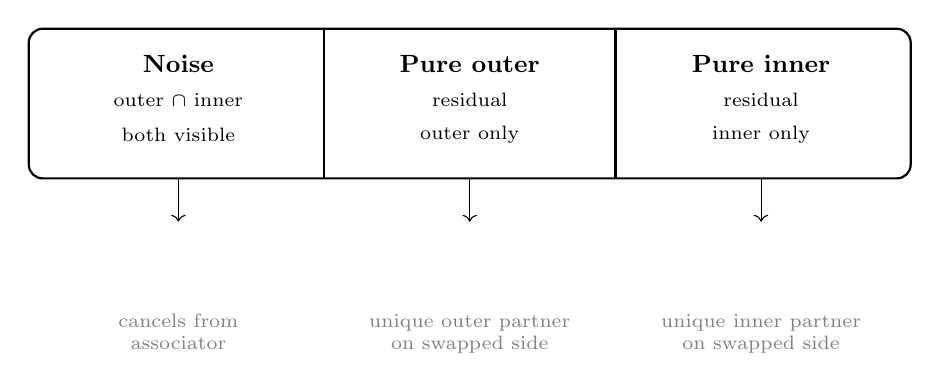
\begin{tikzpicture}[font=\small]
  % outer rectangle
  \draw[thick,rounded corners=5pt] (-5.6,-1) rectangle (5.6,0.9);
  % dividers
  \draw[thick] (-1.85,-1)--(-1.85,0.9);
  \draw[thick] ( 1.85,-1)--( 1.85,0.9);
  % sector labels
  \node[align=center] at (-3.7, 0.45) {\textbf{Noise}};
  \node[align=center,font=\scriptsize] at (-3.7, 0.0) {outer $\cap$ inner};
  \node[align=center,font=\scriptsize] at (-3.7,-0.45) {both visible};
  \node[align=center] at (0, 0.45) {\textbf{Pure outer}};
  \node[align=center,font=\scriptsize] at (0, 0.0) {residual};
  \node[align=center,font=\scriptsize] at (0,-0.45) {outer only};
  \node[align=center] at (3.7, 0.45) {\textbf{Pure inner}};
  \node[align=center,font=\scriptsize] at (3.7, 0.0) {residual};
  \node[align=center,font=\scriptsize] at (3.7,-0.45) {inner only};
  % annotation arrows below
  \draw[->] (-3.7,-1) -- (-3.7,-1.55);
  \node[font=\scriptsize,gray,below=1.6cm of {(-3.7,-1)},align=center]
    {cancels from\\associator};
  \draw[->] (0,-1) -- (0,-1.55);
  \node[font=\scriptsize,gray,below=1.6cm of {(0,-1)},align=center]
    {unique outer partner\\on swapped side};
  \draw[->] (3.7,-1) -- (3.7,-1.55);
  \node[font=\scriptsize,gray,below=1.6cm of {(3.7,-1)},align=center]
    {unique inner partner\\on swapped side};
\end{tikzpicture}
\end{center}
\noindent\small
The three sectors partition the left contribution classes at any fixed
output $w$. Noise classes carry both outer and inner support and cancel
from the associator by the \texttt{outer\_comm\_inner} identification.
The elimination of mixed residual classes (proved above) ensures that
the pure outer and pure inner sectors are exhaustive among residual classes.
Each residual class then has a unique partner on the swapped right side,
yielding the class-level pre-Lie identity.

\begin{remark}
This is the decisive structural step in the whole proof. Once mixed residual
classes disappear, the residual sector becomes typed and rigid, and the final
pre-Lie comparison reduces to separate outer and inner transport theorems.
\end{remark}

\subsection{Unique typed partners}

\begin{theorem}[Unique typed partner theorem]
Let \(q\in \CL(x,y,z;w)\) be residual.
\begin{enumerate}[label=\textup{(\roman*)}]
\item If \(q\) is pure outer, then there exists a unique pure outer class
\(q'\in \CR(x,y,z;w)\) corresponding to \(q\).
\item If \(q\) is pure inner, then there exists a unique pure inner class
\(q'\in \CR(x,y,z;w)\) corresponding to \(q\).
\end{enumerate}
\end{theorem}

\begin{proof}
Suppose first that \(q\) is pure outer. Then \(q\) has outer support, so the
outer transport theorem produces a swapped right-outer class \(q'\)
corresponding to \(q\). Uniqueness among right-outer classes is built into the
same transport theorem, since the transport maps are mutually inverse on the
outer-supported sector.

It remains to check that the transported class is again pure outer on the
swapped side. If it were noise, then \(q\) itself would already belong to the
noise sector, because noise is exactly the quotient-trivial part of the
comparison relation. That contradicts residuality. If instead \(q'\) carried an
inner presentation as well, then transporting that inner information back to
the left would furnish both outer and inner support for \(q\), making \(q\) a
mixed residual class. This is impossible by elimination of mixed residual
classes. Hence \(q'\) is pure outer.

The proof for pure inner classes is the same, using the inner transport theorem
in place of the outer one. Starting from a pure inner residual class \(q\), the
inner transport map produces a unique swapped right-inner class \(q'\). Residual
classes cannot transport to noise, and if \(q'\) also carried outer support,
transporting back would make \(q\) mixed residual, again impossible. Thus
\(q'\) is pure inner, and uniqueness follows from the inverse inner transport.
\end{proof}

\begin{theorem}[Residual classes seen from the swapped side]
Every residual swapped-right contribution class arises from a pure residual
left contribution class.
\end{theorem}

\begin{proof}
Let \(q'\) be a residual swapped-right contribution class. The class-level
decomposition on the swapped side says that every swapped-right contribution
class is either noise or residual with a left partner. Since \(q'\) is
assumed residual, the noise alternative is excluded. Therefore there exists a
left contribution class \(q\) corresponding to \(q'\) under the swapped
comparison relation.

Moreover, the decomposition theorem identifies such a left partner as residual.
By residual purity, every residual left class is either pure outer or pure
inner. Hence \(q\) is a pure residual left class, as required.
\end{proof}

\section{The class-level pre-Lie identity}

\subsection{Associator contributions at a fixed output}

\begin{definition}
For proof trees \(x,y\), define the \emph{primitive class-level product
support} by
\[
\mathsf{Prod}(x,y) := \{\,w \in \PTree : w\in \Graft(x,y)\,\}.
\]
\end{definition}

\begin{remark}
This is not yet a quotient object. It is simply the set of outputs occurring in
one-step grafting. The quotient enters only in the analysis of how these
outputs receive graft-pair associator contributions.
\end{remark}

\begin{definition}
Fix \(x,y,z,w\). The \emph{class-level associator at output \(w\)} is the
assertion that left contribution classes to \(w\) decompose into noise, pure
outer residual classes, and pure inner residual classes, and that these three
sectors compare with the swapped side exactly as described by the noise,
outer-transport, and inner-transport theorems.
\end{definition}

\begin{theorem}[Class-level associator shape]
For every \(x,y,z,w\), the class-level associator at output \(w\) holds.
\end{theorem}

\begin{proof}
Fix \(x,y,z,w\). Let \(q\) be a left contribution class at output \(w\). By the
noise/residual decomposition, \(q\) is either noise or residual. If \(q\) is
residual, then by residual purity it is either pure outer or pure inner. Thus
every left contribution class belongs to one of the three sectors appearing in
the definition of the class-level associator.

Next consider how these sectors compare with the swapped side. Noise classes
are harmless by definition: they are exactly those classes whose left/right
discrepancy is already quotient-trivial, so they contribute no genuine
asymmetry to the associator. If \(q\) is pure outer residual, then by the
unique typed partner theorem it has a unique pure outer partner on the swapped
side. If \(q\) is pure inner residual, the same theorem gives a unique pure
inner partner on the swapped side.

Finally, let \(q'\) be a swapped-right contribution class. If \(q'\) is
residual, then by the preceding theorem it arises from a pure residual left
class. Thus no non-noise swapped-right class lies outside the pure residual
image of the left side. This is exactly the structural assertion encoded in the
definition of the class-level associator at \(w\).
\end{proof}

\begin{theorem}[Class-level pre-Lie comparison]
Fix \(x,y,z,w\). Every left contribution class to the coefficient of \(w\) in
the associator belongs to exactly one of the following three sectors:
\begin{enumerate}[label=\textup{(\roman*)}]
\item quotient-trivial noise;
\item pure outer residual, with a unique swapped pure outer partner;
\item pure inner residual, with a unique swapped pure inner partner.
\end{enumerate}
\end{theorem}

\begin{proof}
Let \(q\) be a left contribution class contributing to the coefficient of
\(w\). By the class-level associator shape just proved, \(q\) lies in one of
three mutually exclusive situations.

If \(q\) is noise, then it belongs to sector~(i), and its contribution is
already quotient-trivial. If \(q\) is pure outer residual, then the unique
typed partner theorem gives a unique swapped pure outer partner, so \(q\)
belongs to sector~(ii). If \(q\) is pure inner residual, the same theorem gives
a unique swapped pure inner partner, so \(q\) belongs to sector~(iii).

These three cases exhaust all left contribution classes, and residual purity
ensures that sectors~(ii) and~(iii) do not overlap. Thus the comparison theorem
is exactly the operational form of the associator-shape theorem.
\end{proof}

\subsection{The main theorem}

\begin{theorem}[Class-level pre-Lie identity]
For all proof trees \(x,y,z\), the class-level associator is symmetric under
interchange of \(x\) and \(y\). Equivalently, for every output tree \(w\), the
contribution classes to
\[
(x\triangleright y)\triangleright z - x\triangleright (y\triangleright z)
\]
are matched, after quotienting by bureaucratic equivalence, with the
contribution classes to
\[
(y\triangleright x)\triangleright z - y\triangleright (x\triangleright z).
\]
\end{theorem}

\begin{proof}
Fix \(w\). By the class-level pre-Lie comparison theorem, every left
contribution class lies in exactly one of three sectors.

\smallskip
\noindent
\emph{Noise.} Noise classes are quotient-trivial by construction and contribute
no genuine asymmetry.

\smallskip
\noindent
\emph{Pure outer residual classes.} These are matched uniquely across the two
bracketings by outer transport.

\smallskip
\noindent
\emph{Pure inner residual classes.} These are matched uniquely across the two
bracketings by inner transport.

\smallskip
Since these three sectors exhaust the left contribution classes at output
\(w\), the class-level associator at \(w\) is symmetric under swapping \(x\)
and \(y\). As \(w\) was arbitrary, the class-level pre-Lie identity follows.
\end{proof}

\begin{remark}
This theorem is the precise endpoint currently established by the formal
development. It is a statement about quotient-invariant associator comparison
at the level of contribution classes. It does not yet claim a fully elaborated
Hopf algebra in the main body of the paper.
\end{remark}

\subsection{Further formally established consequences}

The Lean development proves several sharper statements than are strictly needed
for the narrative route to the main class-level pre-Lie theorem above.  We
record the most mathematically relevant ones here, because they clarify
\emph{where} the quotient enters and \emph{what} has already been proved
independently of the unfinished Hopf-algebra layer.

\begin{definition}
For proof trees \(x\) and \(y\), let
\[
\mathrm{Supp}(x,y):=\{\,w\in \PTree \mid \text{$w$ occurs as a one-step graft
output of $x$ into $y$}\,\}.
\]
Equivalently, \(\mathrm{Supp}(x,y)\) is the support set of the primitive
class-level product.
\end{definition}

\begin{proposition}[Finite one-step support]
For every pair of proof trees \(x,y\), the set \(\mathrm{Supp}(x,y)\) is
finite.
\end{proposition}

\begin{proof}
Every one-step graft output is obtained by choosing a leaf of \(y\) whose
interface matches the conclusion of \(x\), and then replacing that leaf by the
tree \(x\). Since \(y\) has only finitely many leaves, there are only finitely
many admissible one-step grafts of \(x\) into \(y\). Hence the set of outputs
\(\mathrm{Supp}(x,y)\) is finite.
\end{proof}

\begin{proposition}[Support bridge between raw linearization and class-level product]
Let \(\mathbb Z[\PTree]\) be the free abelian group on proof trees, and let
\(e_x,e_y\) denote the basis vectors corresponding to \(x\) and \(y\). Then for
every proof tree \(w\),
\[
w\in \operatorname{supp}(e_x \triangleright e_y)
\quad\Longleftrightarrow\quad
w\in \mathrm{Supp}(x,y).
\]
In particular, the quotient does not alter the \emph{one-step} output set of
proof composition.  Any obstruction to a raw pre-Lie law must therefore occur
at the level of \emph{two-step witness comparison}, i.e.\ in the identity
criteria for derivation histories rather than in the existence of one-step
composites.
\end{proposition}

\begin{proof}
By construction of the raw bilinear grafting product on \(\mathbb Z[\PTree]\),
the product \(e_x\triangleright e_y\) is the formal sum of all one-step
matching-leaf graft outputs of \(x\) into \(y\), counted with multiplicity.
Equivalently,
\[
e_x\triangleright e_y=\sum_{u\in \PTree} m_{x,y}(u)\,e_u,
\]
where \(m_{x,y}(u)\) is the number of admissible graftings producing the tree
\(u\). In particular, the coefficient of \(e_w\) is exactly the number of
occurrences of \(w\) among the one-step outputs. Therefore
\[
w\in \operatorname{supp}(e_x\triangleright e_y)
\quad\Longleftrightarrow\quad
m_{x,y}(w)\neq 0
\quad\Longleftrightarrow\quad
w\in \mathrm{Supp}(x,y).
\]
This proves the equivalence.
\end{proof}

\begin{theorem}[Trichotomy of contribution classes]
Fix proof trees \(x,y,z,w\). Every left contribution class at output \(w\)
belongs to one of the following three sectors:
\begin{enumerate}[label=\textup{(\roman*)}]
\item quotient-trivial overlap noise;
\item pure outer residual;
\item pure inner residual.
\end{enumerate}
Equivalently, the mixed residual sector is empty.
\end{theorem}

\begin{proof}
Fix a left contribution class \(q\) at output \(w\). By the quotient-level
decomposition proved earlier, \(q\) is either overlap noise or residual. If it
is noise, we are done. So suppose \(q\) is residual.

Residual classes admit a second decomposition according to which kinds of
left-side support they carry: pure outer, pure inner, or mixed. Thus the only
possible obstruction to the announced trichotomy is the existence of a mixed
residual class. We now exclude that possibility.

Assume \(q\) were mixed residual. Then \(q\) would carry both outer and inner
left support while, by residuality, avoiding the quotient-trivial overlap
sector. The formal geometry of two-step grafts then forces every outer
representative of \(q\) into the dependent-address regime: if an outer
representative had incomparable addresses, it would already lie in the
commuting/transported sector and hence fail to be mixed residual. But once the
addresses are comparable, the explicit witness analysis constructs right-side
support from the same class, contradicting the defining characterization of the
open mixed fragment as carrying no genuine right-side partner. Hence the mixed
residual sector is empty.

Therefore every residual left class is either pure outer or pure inner. Adding
back the overlap-noise case yields the claimed trichotomy.
\end{proof}

\begin{definition}[Quotient sectors and transport maps]
Fix proof trees \(x,y,z,w\), and write
\[
\mathcal L:=\CL(x,y,z;w),
\qquad
\mathcal R:=\CR(x,y,z;w)
\]
for the left and swapped-right contribution classes at output \(w\).  Inside
these quotient sets we distinguish the following subsets:
\[
\mathcal L_{\mathrm{out}}
:=
\{\,q\in \mathcal L \mid \text{$q$ has outer support}\,\},
\]
\[
\mathcal R_{\mathrm{out}}
:=
\{\,q'\in \mathcal R \mid \text{$q'$ has swapped-right outer support}\,\},
\]
\[
\mathcal L_{\mathrm{pin}}
:=
\{\,q\in \mathcal L \mid \text{$q$ is pure inner residual}\,\},
\]
\[
\mathcal R_{\mathrm{in,res}}
:=
\{\,q'\in \mathcal R \mid \text{$q'$ is residual and has swapped-right inner support}\,\}.
\]
The witness-level outer transport and its inverse descend to quotient maps
\[
T_{\mathrm{out}}:\mathcal L_{\mathrm{out}}\to \mathcal R_{\mathrm{out}},
\qquad
S_{\mathrm{out}}:\mathcal R_{\mathrm{out}}\to \mathcal L_{\mathrm{out}}.
\]
Likewise the witness-level inner transport and its inverse descend to maps
\[
T_{\mathrm{in}}:\mathcal L_{\mathrm{pin}}\to \mathcal R_{\mathrm{in,res}},
\qquad
S_{\mathrm{in}}:\mathcal R_{\mathrm{in,res}}\to \mathcal L,
\]
where \(T_{\mathrm{in}}\) is obtained by restricting the quotient-level inner
transport to pure inner residual left classes, and \(S_{\mathrm{in}}\) is the
corresponding inverse transport on residual swapped-right inner classes.
\end{definition}

\begin{proposition}[Transport on quotient sectors]
With notation as above:
\begin{enumerate}[label=\textup{(\roman*)}]
\item The outer transport maps are mutually inverse:
\[
S_{\mathrm{out}}\circ T_{\mathrm{out}}=\mathrm{id}_{\mathcal L_{\mathrm{out}}},
\qquad
T_{\mathrm{out}}\circ S_{\mathrm{out}}=\mathrm{id}_{\mathcal R_{\mathrm{out}}}.
\]
In particular, \(T_{\mathrm{out}}\) is a bijection from
\(\mathcal L_{\mathrm{out}}\) onto \(\mathcal R_{\mathrm{out}}\).
\item For every \(q\in \mathcal L_{\mathrm{pin}}\),
\[
S_{\mathrm{in}}(T_{\mathrm{in}}(q))=q.
\]
Moreover, if \(t\in \mathcal R_{\mathrm{in,res}}\) satisfies
\[
S_{\mathrm{in}}(t)=q,
\]
then \(t=T_{\mathrm{in}}(q)\).
\end{enumerate}
\end{proposition}

\begin{proof}
For the outer sector, the formal quotient transport theorems construct
\(T_{\mathrm{out}}\) and \(S_{\mathrm{out}}\) and prove directly that they are
inverse on outer-supported classes. Concretely, if
\(q\in \mathcal L_{\mathrm{out}}\), then transport to the swapped-right outer
side and transport back returns the original quotient class:
\[
S_{\mathrm{out}}(T_{\mathrm{out}}(q))=q.
\]
Similarly, if \(t\in \mathcal R_{\mathrm{out}}\), then
\[
T_{\mathrm{out}}(S_{\mathrm{out}}(t))=t.
\]
These two identities are exactly the statement that \(T_{\mathrm{out}}\) and
\(S_{\mathrm{out}}\) are mutually inverse bijections between
\(\mathcal L_{\mathrm{out}}\) and \(\mathcal R_{\mathrm{out}}\).

For the inner sector, let \(q\in \mathcal L_{\mathrm{pin}}\). By definition,
\(q\) is pure inner residual, hence in particular inner-supported. Therefore the
quotient-level inner transport is defined on \(q\). The formal inner transport
theorem shows that transporting to the swapped side and then transporting back
recovers the original class:
\[
S_{\mathrm{in}}(T_{\mathrm{in}}(q))=q.
\]
The same theorem also shows that \(T_{\mathrm{in}}(q)\) carries swapped-right
inner support, while the residuality part of the pure-inner hypothesis is
preserved by transport; thus \(T_{\mathrm{in}}(q)\in \mathcal R_{\mathrm{in,res}}\).

Now let \(t\in \mathcal R_{\mathrm{in,res}}\) satisfy \(S_{\mathrm{in}}(t)=q\).
Applying \(T_{\mathrm{in}}\) to both sides gives
\[
T_{\mathrm{in}}(S_{\mathrm{in}}(t))=T_{\mathrm{in}}(q).
\]
But \(t\) is a swapped-right inner class, so the quotient-level inverse law for
inner transport applies and yields \(T_{\mathrm{in}}(S_{\mathrm{in}}(t))=t\).
Hence \(t=T_{\mathrm{in}}(q)\), as required.
\end{proof}

\begin{theorem}[Unique partners in the pure sectors]
Fix proof trees \(x,y,z,w\).
\begin{enumerate}[label=\textup{(\roman*)}]
\item For every \(q\in \mathcal L_{\mathrm{out}}\) there exists a unique
\(t\in \mathcal R_{\mathrm{out}}\) such that
\[
S_{\mathrm{out}}(t)=q.
\]
Equivalently, every outer-supported left contribution class has a unique
swapped-right outer partner.
\item For every \(q\in \mathcal L_{\mathrm{pin}}\) there exists a unique
\(t\in \mathcal R_{\mathrm{in,res}}\) such that
\[
S_{\mathrm{in}}(t)=q.
\]
Equivalently, every pure inner residual left contribution class has a unique
residual swapped-right inner partner.
\end{enumerate}
\end{theorem}

\begin{proof}
For \textup{(i)}, let \(q\in \mathcal L_{\mathrm{out}}\). Set
\[
t:=T_{\mathrm{out}}(q)\in \mathcal R_{\mathrm{out}}.
\]
Then by the outer inverse law,
\[
S_{\mathrm{out}}(t)=S_{\mathrm{out}}(T_{\mathrm{out}}(q))=q.
\]
So a partner exists. If \(t'\in \mathcal R_{\mathrm{out}}\) is any other class
with \(S_{\mathrm{out}}(t')=q\), then applying \(T_{\mathrm{out}}\) gives
\[
t'=T_{\mathrm{out}}(S_{\mathrm{out}}(t'))=T_{\mathrm{out}}(q)=t,
\]
using the right-inverse identity on \(\mathcal R_{\mathrm{out}}\). Hence the
partner is unique.

For \textup{(ii)}, let \(q\in \mathcal L_{\mathrm{pin}}\). Set
\[
t:=T_{\mathrm{in}}(q)\in \mathcal R_{\mathrm{in,res}}.
\]
By the inner inverse law proved in the preceding proposition, one has
\[
S_{\mathrm{in}}(t)=S_{\mathrm{in}}(T_{\mathrm{in}}(q))=q.
\]
So a residual swapped-right inner partner exists. If
\(t'\in \mathcal R_{\mathrm{in,res}}\) also satisfies \(S_{\mathrm{in}}(t')=q\),
then the uniqueness clause of the preceding proposition gives
\[
t'=T_{\mathrm{in}}(q)=t.
\]
Thus the residual swapped-right inner partner is unique.
\end{proof}

\begin{proposition}[Where the quotient enters]
The quotient affects the associator comparison only at the level of
\emph{two-step derivation histories}; it does not alter the \emph{one-step}
grafting support.
\end{proposition}

\begin{proof}
The one-step statement was proved earlier: for proof trees \(x,y\), the support
of the raw bilinear product \(e_x\triangleright e_y\in \mathbb Z[\PTree]\) is
exactly the set \(\mathrm{Supp}(x,y)\) of one-step graft outputs. In
particular, the existence of one-step composites is already determined on the
raw free abelian group of proof trees.

The quotient enters only when one compares \emph{two-step} composites. For
fixed \(x,y,z,w\), let \(\mathrm{Code}(x,y,z;w)\) denote the set of raw
two-step graft-pair codes with final output \(w\), and let
\[
\pi_{x,y,z;w}:\mathrm{Code}(x,y,z;w)\twoheadrightarrow
\mathrm{Code}(x,y,z;w)/{\sim_{\mathrm b}}
\]
be the quotient map by bureaucratic equivalence. By definition, the generators
of this equivalence are the elementary commutation and transport maps introduced
earlier; and by the proposition ``bureaucratic equivalence preserves the
composite tree'', each generating move preserves the final output tree. Hence
every fibre of \(\pi_{x,y,z;w}\) consists of raw two-step derivation histories
with the same composite output.

Therefore quotienting does not create or destroy one-step graft outputs. What it
changes is the identity relation on ordered pairs of grafts occurring in the
associator: schedules that differ only by bureaucratic commutation or
reassociation are identified, and the overlap-noise sector becomes
quotient-trivial. This is exactly the point at which the proof-theoretic
bureaucracy of derivations enters the pre-Lie argument.
\end{proof}

\section{Preparatory coproduct data and Hopf outlook}

The formal development also defines a cut-based coproduct datum on proof trees.
This section records the mathematical shape of that construction and its
relationship to the Hopf-algebraic route.

\begin{definition}[Admissible cuts]
Let \(t\in\PTree\). An \emph{admissible cut} of \(t\) is a finite set
\[
C\subseteq \Addr(t)
\]
such that:
\begin{enumerate}[label=\textup{(\roman*)}]
\item every \(a\in C\) is a valid address of \(t\);
\item \(C\) is an antichain for the prefix order, i.e. if \(a,b\in C\) and
\(a\neq b\), then neither \(a\preceq b\) nor \(b\preceq a\).
\end{enumerate}
Equivalently, along any path from the root to a leaf, at most one address is
cut.
\end{definition}

\begin{definition}[Pruned forest and remainder]
Let \(C\) be an admissible cut of \(t\). The \emph{pruned forest} is
\[
P_C(t):=\prod_{a\in C} t\downarrow_a
\in \Forest(\PTree),
\]
with the convention that the empty product is the empty forest \(1\).

The \emph{remainder} or \emph{trunk} \(R_C(t)\) is the proof tree obtained
from \(t\) by replacing, for each \(a\in C\), the rooted subtree
\(t\downarrow_a\) by its root sequent regarded as a leaf. Since the addresses
in \(C\) are pairwise incomparable, these replacements occur in disjoint
subtrees and hence are independent of order.
\end{definition}

\begin{definition}[Cut coproduct datum]
The Grossman--Larson style cut datum on proof trees is the formal sum
\[
\Delta_{\mathrm{cut}}(t)
:=
\sum_{C\in \operatorname{Adm}(t)}
P_C(t)\otimes R_C(t),
\]
where \(\operatorname{Adm}(t)\) denotes the finite set of admissible cuts of
\(t\). The empty cut contributes
\[
1\otimes t.
\]
If the root cut is included among admissible cuts, it contributes
\[
t\otimes 1,
\]
where \(1\) is the empty proof tree/forest unit on the appropriate carrier.
If root cuts are omitted, the \(t\otimes 1\) term may instead be adjoined
separately, as in the usual Connes--Kreimer convention.
\end{definition}

\begin{proposition}
Every proof tree admits at least one cut decomposition.
\end{proposition}

\begin{proof}
The empty cut is always admissible, and it yields the trivial decomposition
into the empty forest together with the original tree.
\end{proof}

\begin{lemma}[Restriction of a cut to a child]
Let
\[
t=R(t_1,\ldots,t_n)
\]
be an arity-correct proof tree with root rule \(R\) and immediate subtrees
\(t_1,\ldots,t_n\). If \(C\in\operatorname{Adm}(t)\), then for each
\(1\le i\le n\) the set
\[
C_i:=\{\,a\in\Addr(t_i): i\cdot a\in C\,\}
\]
is an admissible cut of \(t_i\).
\end{lemma}

\begin{proof}
Validity of addresses is inherited by passing from an address \(i\cdot a\) in
the whole tree to the corresponding address \(a\) in the \(i\)-th child
subtree. For the antichain condition, suppose \(a,b\in C_i\) are comparable in
\(\Addr(t_i)\). Then \(i\cdot a\) and \(i\cdot b\) are comparable in
\(\Addr(t)\). Since both lie in \(C\), admissibility of \(C\) forces
\(i\cdot a=i\cdot b\), hence \(a=b\). Thus \(C_i\) is an antichain.
\end{proof}

\begin{lemma}[Node cut decomposition]
Let \(t=R(t_1,\ldots,t_n)\) be arity-correct and let \(C\) be an admissible cut
which does not cut the root. Then \(C\) is uniquely determined by the tuple of
child cuts
\[
(C_1,\ldots,C_n),
\qquad C_i\in\operatorname{Adm}(t_i),
\]
and conversely every tuple of admissible child cuts determines an admissible
cut of \(t\) not cutting the root.
\end{lemma}

\begin{proof}
The forward direction is the restriction lemma. Conversely, given admissible
cuts \(C_i\subseteq\Addr(t_i)\), form
\[
C:=\bigcup_{i=1}^n \{\,i\cdot a:a\in C_i\,\}.
\]
Each address in \(C\) is valid in \(t\). If two such addresses have different
first child indices, they lie in disjoint branches and are incomparable. If
they have the same first child index, comparability in \(t\) reduces to
comparability in the corresponding child tree, and the antichain property of
\(C_i\) applies. Thus \(C\) is admissible. The two constructions are inverse
because every non-root address of a node tree has a unique first child index.
\end{proof}

\begin{remark}
This node decomposition is the combinatorial heart of the cut construction.
It is the rooted-tree analogue of decomposing an admissible cut of a tree into
admissible cuts of the immediate branches. In the proof-theoretic setting the
number of branches is not arbitrary: it is fixed by the arity of the inference
rule at the root.
\end{remark}

\begin{proposition}[Recursive form of the cut coproduct]
Let \(t=R(t_1,\ldots,t_n)\) be arity-correct. Up to the convention about
whether the root cut is included in \(\operatorname{Adm}(t)\), the non-root
part of \(\Delta_{\mathrm{cut}}(t)\) is obtained by summing over tuples of
admissible child cuts:
\[
\sum_{C_1,\ldots,C_n}
\bigl(P_{C_1}(t_1)\cdots P_{C_n}(t_n)\bigr)
\otimes
R\bigl(R_{C_1}(t_1),\ldots,R_{C_n}(t_n)\bigr).
\]
\end{proposition}

\begin{proof}
By the node cut decomposition, admissible non-root cuts of \(t\) are in
bijection with tuples of admissible cuts of the immediate subtrees. Under this
bijection, the pruned forest is the product of the pruned forests of the child
cuts, and the remainder tree is obtained by applying the same root rule \(R\)
to the child remainders.
\end{proof}

\begin{theorem}[Coassociativity reduces to nested cut decomposition]
The coassociativity equation for the cut coproduct,
\[
(\Delta_{\mathrm{cut}}\otimes \mathrm{id})\Delta_{\mathrm{cut}}(t)
=
(\mathrm{id}\otimes \Delta_{\mathrm{cut}})\Delta_{\mathrm{cut}}(t),
\]
is equivalent to the statement that a two-stage cut of \(t\) can be uniquely
read either as:
\begin{enumerate}[label=\textup{(\roman*)}]
\item first cutting a family of subtrees and then cutting inside the pruned
forest; or
\item first cutting the remainder tree and then collecting the resulting
pruned pieces.
\end{enumerate}
\end{theorem}

\begin{proof}[Proof sketch]
Both sides enumerate the same data: a finite family of pairwise compatible cut
addresses together with a choice of which cut components are regarded as
first-stage and which as second-stage. The antichain condition ensures that
cut subtrees are either disjoint or nested in the controlled way required by
admissibility. The node decomposition lemma reduces the comparison to the
corresponding statement on the immediate child trees, so the proof proceeds by
height induction on \(t\). The base case is a leaf, where only the empty and
possibly root cuts occur. The inductive step is exactly the arity-indexed
node case above.
\end{proof}

\begin{remark}
The formal project is presently pursuing this theorem through the structural
cut lemmas just stated. Earlier explicit computations of coproducts on small
trees are useful regression tests, but they are not the proof strategy. The
proof strategy is the height induction controlled by rule arity and node cut
decomposition.
\end{remark}

\begin{remark}
This coproduct material is preparatory rather than central in the present
paper. It shows that the proof-tree side already carries the decomposition data
expected of a Connes--Kreimer style coproduct, but we do not yet prove the
full compatibility theorems needed for a Hopf algebra in the body of the
paper.
\end{remark}

\begin{remark}
There are two natural routes from the present work to Hopf algebra.
\begin{enumerate}[label=\textup{(\roman*)}]
\item A direct cut/grafting route, in which one relates the cut-based coproduct
to proof-tree grafting itself.
\item An Oudom--Guin route, in which the class-level pre-Lie structure proved
here is first extended to a symmetric algebra and only then combined with a
primitive coproduct.
\end{enumerate}
The second route is the one most strongly suggested by the present formal
results, and it is the route we have in mind when the abstract mentions Hopf
algebraic consequences.
\end{remark}

\begin{definition}[Pre-Lie difference relations]
Let \(V=\ZZ\langle\PTree\rangle\) with grafting product
\(\triangleright\). For proof trees \(x,y,z\), define the \emph{pre-Lie
difference}
\[
D(x,y,z):=
(x\triangleright y)\triangleright z
-x\triangleright (y\triangleright z)
-(x\triangleright z)\triangleright y
+x\triangleright (z\triangleright y).
\]
Let \(R_{\mathrm{pl}}\subseteq V\) be the subgroup generated by all
\(D(x,y,z)\). A \emph{stable pre-Lie relation submodule} is a subgroup
\(R_{\mathrm{st}}\subseteq V\) containing \(R_{\mathrm{pl}}\) and closed under
left and right grafting by tree generators:
\[
u\triangleright r,\ r\triangleright u\in R_{\mathrm{st}}
\qquad
(u\in\PTree,\ r\in R_{\mathrm{st}}).
\]
\end{definition}

\begin{remark}
The adjective ``stable'' is important. Quotienting merely by the formal
pre-Lie differences ensures that the pre-Lie identity holds in the quotient,
but it does not by itself ensure that grafting is well-defined on quotient
classes. Stability is the algebraic condition that makes the product descend.
\end{remark}

\begin{proposition}[Product descent through a stable quotient]
Let \(Q:=V/R_{\mathrm{st}}\). If \(R_{\mathrm{st}}\) is stable under left and
right grafting, then \(\triangleright\) descends to a well-defined bilinear
product
\[
\bar{\triangleright}:Q\otimes Q\to Q.
\]
Moreover, the descended product satisfies the right pre-Lie identity.
\end{proposition}

\begin{proof}
If \(x-x'\in R_{\mathrm{st}}\) and \(y-y'\in R_{\mathrm{st}}\), then by
bilinearity
\[
x\triangleright y-x'\triangleright y'
=(x-x')\triangleright y+x'\triangleright (y-y')
\in R_{\mathrm{st}},
\]
using stability. Hence the product is independent of representatives. Since
all pre-Lie differences \(D(x,y,z)\) lie in \(R_{\mathrm{st}}\), their images
in \(Q\) vanish, which is exactly the right pre-Lie identity for the descended
product.
\end{proof}

\begin{definition}[Coideal condition]
Let \((V,\Delta,\varepsilon)\) be a coalgebra-like structure on the raw
linear tree module. A subgroup \(R\subseteq V\) is a \emph{coideal} if
\[
\Delta(R)\subseteq R\otimes V+V\otimes R
\qquad\text{and}\qquad
\varepsilon(R)=0.
\]
\end{definition}

\begin{proposition}[Coalgebra descent criterion]
If \(R\subseteq V\) is a coideal, then \(\Delta\) and \(\varepsilon\) descend
to well-defined maps
\[
\bar{\Delta}:V/R\to (V/R)\otimes (V/R),
\qquad
\bar{\varepsilon}:V/R\to \ZZ.
\]
If \(\Delta\) is coassociative and counital on \(V\), then
\(\bar{\Delta}\) is coassociative and counital on \(V/R\).
\end{proposition}

\begin{proof}
Let \(\pi:V\to V/R\) be the quotient map. The condition
\(\Delta(R)\subseteq R\otimes V+V\otimes R\) says precisely that
\((\pi\otimes\pi)\Delta(r)=0\) for every \(r\in R\). Thus
\((\pi\otimes\pi)\Delta\) is constant on cosets and factors uniquely through
\(\pi\), giving \(\bar{\Delta}\). The condition \(\varepsilon(R)=0\) gives the
same factorization for the counit. Coassociativity and counitality descend
because they are equations of maps out of \(V/R\), and precomposing with the
surjection \(\pi\) reduces them to the corresponding equations on \(V\).
\end{proof}

\begin{remark}
For the direct cut route, the essential missing theorem is therefore not just
that \(\Delta_{\mathrm{cut}}\) is coassociative on raw trees. One must also
show that the proof-theoretic relation submodule is a coideal:
\[
\Delta_{\mathrm{cut}}(R_{\mathrm{st}})
\subseteq
R_{\mathrm{st}}\otimes V+V\otimes R_{\mathrm{st}}.
\]
This is the precise algebraic form of the statement that cut decomposition is
compatible with the proof-theoretic quotient.
\end{remark}

\begin{definition}[Stable quotient and enveloping algebra]
Let \(R_{\mathrm{st}}\subseteq \ZZ\langle\PTree\rangle\) be the subgroup
generated by the stable pre-Lie difference relations, and set
\[
Q:=\ZZ\langle\PTree\rangle / R_{\mathrm{st}}.
\]
Write \([x]\in Q\) for the class of the basis element \(e_x\). The
class-level pre-Lie product on \(Q\) induces a Lie bracket
\[
[u,v]:=u\triangleright v-v\triangleright u,
\]
and we denote the resulting Lie algebra by \(Q_{\mathrm{Lie}}\). Its
universal enveloping algebra is denoted
\[
U(Q):=U(Q_{\mathrm{Lie}}).
\]
Finally, write
\[
\iota:Q\to U(Q)
\]
for the canonical linear map.
\end{definition}

\begin{theorem}[Conditional descent of primitive generator data]
Let \(Q\) be the stable quotient of the free abelian group on proof trees by
the pre-Lie difference stable relations, let \(U(Q)\) be the universal
enveloping algebra of the induced Lie algebra, and let
\(\iota:Q\to U(Q)\) denote the canonical map. Suppose that one is given
generator-level data
\[
\Delta_0:\PTree\to U(Q)\otimes U(Q),
\qquad
\varepsilon_0:\PTree\to \mathbb Z
\]
whose induced linear maps on \(\mathbb Z[\PTree]\) vanish on the stable
relations. Then there exist well-defined descended linear maps
\[
\Delta:Q\to U(Q)\otimes U(Q),
\qquad
\varepsilon:Q\to \mathbb Z
\]
whose values on tree generators are exactly those prescribed by
\(\Delta_0\) and \(\varepsilon_0\). In particular, if
\[
\Delta_0(x)=\iota([x])\otimes 1 + 1\otimes \iota([x]),
\qquad
\varepsilon_0(x)=0
\]
on generators, then the descended maps satisfy the same formulas on generator
classes:
\[
\Delta([x])=\iota([x])\otimes 1 + 1\otimes \iota([x]),
\qquad
\varepsilon([x])=0.
\]
\end{theorem}

\begin{proof}
Let
\[
\pi:\mathbb Z[\PTree]\twoheadrightarrow Q
\]
be the quotient map. The hypotheses say precisely that the linear extensions of
\(\Delta_0\) and \(\varepsilon_0\) to \(\mathbb Z[\PTree]\) vanish on the
stable relation submodule. Therefore each of them factors uniquely through the
quotient \(Q\). In other words, there exist unique linear maps
\[
\Delta:Q\to U(Q)\otimes U(Q),
\qquad
\varepsilon:Q\to \mathbb Z
\]
such that
\[
\Delta\circ \pi = \widetilde{\Delta}_0,
\qquad
\varepsilon\circ \pi = \widetilde{\varepsilon}_0,
\]
where \(\widetilde{\Delta}_0\) and \(\widetilde{\varepsilon}_0\) denote the
linear extensions of the generator data.

Evaluating these identities on a basis tree \(x\) gives
\[
\Delta([x])=\Delta(\pi(e_x))=\widetilde{\Delta}_0(e_x)=\Delta_0(x),
\qquad
\varepsilon([x])=\varepsilon(\pi(e_x))=\widetilde{\varepsilon}_0(e_x)
=\varepsilon_0(x).
\]
Hence the descended maps agree with the prescribed generator formulas. The
primitive-generator case is obtained by substituting
\(\Delta_0(x)=\iota([x])\otimes 1+1\otimes \iota([x])\) and
\(\varepsilon_0(x)=0\).
\end{proof}

\begin{theorem}[Extension principle from generators]
Let \(V=\mathbb Z[\PTree]\). Any bilinear product on \(V\) whose values on tree
generators satisfy the right pre-Lie identity extends to a right pre-Lie
algebra structure on all of \(V\). Likewise, any additive weight law verified
on generator products extends to all homogeneous elements of \(V\).
\end{theorem}

\begin{proof}
Write
\[
A(a,b,c):=(a\cdot b)\cdot c-a\cdot (b\cdot c)
\]
for the associator of the bilinear product. The difference
\[
T(a,b,c):=A(a,b,c)-A(a,c,b)
\]
is trilinear in \(a,b,c\), because the product is bilinear. If \(T\) vanishes
on all triples of basis elements \(e_x,e_y,e_z\), then by trilinearity it
vanishes on all finite \(\mathbb Z\)-linear combinations of such basis
elements. Since \(V=\mathbb Z[\PTree]\) is the free abelian group on the trees,
every element of \(V\) is a finite sum of basis vectors, so \(T=0\) on all of
\(V^3\). This is exactly the right pre-Lie identity on \(V\).

The grading statement is analogous. Let \(V_n\subseteq V\) be the subgroup
generated by trees of weight \(n\). If the generator-level law says that the
product of a weight-\(m\) basis tree and a weight-\(n\) basis tree lies in
\(V_{m+n}\), then bilinearity implies that the product of arbitrary homogeneous
elements of degrees \(m\) and \(n\) is a finite sum of terms each lying in
\(V_{m+n}\). Hence the whole product lies in \(V_{m+n}\), so the weight law
extends from generators to all homogeneous elements.
\end{proof}

\begin{remark}[Current state of the Oudom--Guin development]
The formal development already contains preparatory work toward route~(ii).
The files \texttt{GrossmanLarssonOudomGuinCoalgebra.lean} and
\texttt{GrossmanLarssonOudomGuinHopfRigidity.lean} contain the current
formal infrastructure for the following:
\begin{itemize}
\item a graft-compatible weight function on proof trees, grading every
one-step product output by the reduced-weight law
\(\|w\|=\|x\|+\|y\|\) whenever \(w\in\Graft(x,y)\);
\item a proof that any bilinear product on the linear proof-tree carrier whose
generator-level behaviour matches the quotient pre-Lie law automatically
satisfies the right pre-Lie axiom on the entire carrier \newline 
(\texttt{generatorRightPreLieLaw\_extends});
\item a proof that any such product respects the weight grading on all
homogeneous elements (\texttt{generatorWeightLaw\_extends}).
\end{itemize}
The remaining step for route~(ii) is to construct the specific bilinear
product from the quotient data --- i.e.\ to show that the grafting operation
descends to a well-defined map on the linear carrier that is compatible with
the quotient --- and then to apply the Oudom--Guin theorem to obtain the
enveloping Hopf algebra on the symmetric algebra. The infrastructure is in
place; this is the content of the next paper in this series.
\end{remark}

\begin{remark}[Why the Connes--Kreimer route is not taken]
The direct cut/grafting route~(i) would require the algebraic product to be
the forest product (disjoint union of proof trees). However, a forest of proof
trees has no natural proof-theoretic interpretation: there is no sequent whose
derivation \emph{is} a side-by-side collection of independent proof trees.
Proof composition is sequential --- one proof's conclusion becomes another's
premiss leaf --- not parallel. The grafting product is proof-theoretically
meaningful precisely because it is proof composition. Route~(i) is therefore
not pursued here, though a comparison with Connes--Kreimer-style Hopf algebras
by forgetting the sequent decoration remains an interesting open problem (see
the following remark).
\end{remark}

\begin{remark}
A further comparison problem, not treated here, is to relate the present
structure to familiar rooted-tree Hopf algebras by forgetting some of the
proof-theoretic decoration while retaining the underlying tree and insertion
geometry. Such comparison theorems would strengthen the claim that the present
construction refines, rather than competes with, established combinatorial
Hopf-algebraic frameworks. The key question is whether the Hopf algebra
obtained via the Oudom--Guin route depends essentially on the primitive
relation $\mszero$ --- in the sense that different choices of $\mszero$
yield genuinely non-isomorphic algebraic structures --- or whether the
structure is universal and the logical content enters only through the
choice of basis. Settling this would determine whether the construction
encodes something specifically about nonmonotonic proof theory or merely
recovers a combinatorial object by a proof-theoretic route.
\end{remark}

\begin{remark}[Relation to Foissy's comodule viewpoint]
Foissy's analysis of the Hopf algebra of rooted trees emphasizes that the
coalgebra structure is not merely a bookkeeping device: finite-dimensional
comodules encode how iterated cut decompositions are organized by primitive
pieces, and the whole Hopf algebra admits filtrations and gradings reflecting
this decomposition. This suggests a useful comparison problem for proof trees.
If a finite family of derivations is closed under taking the remainders and
pruned components appearing in \(\Delta_{\mathrm{cut}}\), then its span should
behave like a finite-dimensional comodule over the relevant rooted-tree Hopf
algebra or over its proof-theoretic quotient. In proof-theoretic terms, such a
comodule would package the finite space of subderivations and residual proof
obligations generated by repeatedly cutting a derivation.

This is not used in the present proof of the pre-Lie identity, but it is a
natural source of future invariants. The Loewy-style filtration of a comodule
by trivial quotients has a proof-theoretic reading as a filtration by depth of
nontrivial decomposition: primitive elements correspond to indecomposable
proof-tree contributions, while higher layers record iterated cut structure.
\end{remark}

\begin{remark}[Structural rules as future parameters]
As noted in the introduction, the present paper fixes multiset contexts and
omits weakening and contraction. Each structural rule is a potential parameter.
Adding weakening makes sequent interfaces non-rigid: one could graft into any
leaf by first weakening the context to match. This would change the leaf-matching
constraint fundamentally and is expected to obstruct the coproduct compatibility
rather than the pre-Lie structure. Adding contraction collapses multisets
differing in formula multiplicities, changing which sequents are identified and
potentially breaking the noise/residual separation whose geometry depends on
the counting of matching leaves. Moving from multisets to sequences (removing
the built-in exchange) would add ordered structure to sequents and make the
grafting product sensitive to context ordering in ways that require separate
analysis. A systematic study of which structural rules are obstructions to
Hopf-algebraic compatibility is left for future work.
\end{remark}

\fi

\section{Conclusion}

We have constructed a proof-theoretic route from a primitive consequence
relation to a class-level pre-Lie identity on proof-tree composition.
Formally, the route is
\[
\begin{aligned}
\mszero
&\longrightarrow \NMMS(\mszero)\\
&\longrightarrow \text{proof trees}
\longrightarrow \text{grafting geometry}\\
&\longrightarrow \text{graft-pair quotient}
\longrightarrow \text{class-level pre-Lie identity}.
\end{aligned}
\]

The distinctive point is not merely that rooted trees appear, but that they
appear as proof objects carrying exact sequent interfaces. Grafting is
therefore proof composition, not arbitrary combinatorial insertion. The
graft-pair quotient then isolates what should count as invariant in proof
composition: independent commutations and quotient-trivial overlap disappear as
bureaucracy, while the residual sector becomes pure and rigid enough to satisfy
the class-level pre-Lie identity.

From the standpoint of logic, this means that a nonmonotonic proof theory can
carry nontrivial algebraic structure without first collapsing to a monotone or
structurally saturated setting. From the standpoint of algebra, it shows that
pre-Lie behavior can emerge from proof composition once identity of proof is
handled carefully at the level of graft-pair interactions. The Hopf-theoretic
extensions suggested by the present development are important, but they are
best seen as a next step built on top of the logic result already proved here:
after quotienting bureaucratic symmetries, proof composition on these
nonmonotonic proof trees satisfies a class-level pre-Lie identity.

The quotient is not a stylistic choice. The direct approach to the pre-Lie
identity --- proving that the raw witness counts balance on both sides of the
associator --- was attempted and did not close. The equivalence relation on
graft-pair codes, and in particular the \texttt{outer\_comm\_inner} identification
of comparable-address graftings, is the structure that makes the proof work.
This identification has a proof-theoretic reading: it says that two derivation
histories for the same output proof tree, which look geometrically different at
the address level, should count as the same composition when the relevant graft
sites stand in a dependency relation. The noise/residual separation is then a
precise account of which histories are genuinely the same (noise, canceling from
the associator) and which are genuinely distinct (residual, matched uniquely
across the two bracketings).

The pre-Lie identity is fully machine-verified in Lean~4.  The algebra homomorphisms $\Delta_{\mathrm{split}}$ and $\varepsilon_{\mathrm{split}}$ are constructed as Mathlib \texttt{AlgHom}s.  Coassociativity, the counit laws, and the full Hopf algebra axioms are the principal remaining formal targets; coassociativity reduces to the nested-cut bijection described in Section~\ref{sec:cut-formal}.  The broader programme --- determining which structural rules obstruct Hopf-algebraic compatibility --- remains open and will be pursued in subsequent work.

\begin{thebibliography}{9}

\bibitem{avron1996hypersequents}
A.~Avron.
\newblock The method of hypersequents in the proof theory of propositional
  non-classical logics.
\newblock In W.~Hodges, M.~Hyland, C.~Steinhorn, and J.~Truss, editors,
  \emph{Logic: From Foundations to Applications}, pages 1--32. Oxford University Press, 1996.

\bibitem{grossmanlarsson1989}
R.~Grossman and R.~Larson.
\newblock Hopf-algebraic structure of families of trees.
\newblock \emph{Journal of Algebra}, 126(1):184--210, 1989.

\bibitem{oudomguin2008}
J.-M.~Oudom and D.~Guin.
\newblock On the Lie enveloping algebra of a pre-Lie algebra.
\newblock \emph{Journal of $K$-Theory}, 2(1):147--167, 2008.

\bibitem{conneskireimer1998}
A.~Connes and D.~Kreimer.
\newblock Hopf algebras, renormalization and noncommutative geometry.
\newblock \emph{Communications in Mathematical Physics}, 199(1):203--242, 1998.

\bibitem{milnormoore1965}
J.~Milnor and J.~Moore.
\newblock On the structure of Hopf algebras.
\newblock \emph{Annals of Mathematics}, 81(2):211--264, 1965.

\end{thebibliography}

\end{document}
